\documentclass[letterpaper,12pt,oneside]{book}
%\usepackage[a4paper,includeall,bindingoffset=0cm,margin=2cm,marginparsep=0cm,marginparwidth=0cm]{geometry}
%\usepackage[top=1in, left=0.9in, right=1.25in, bottom=1in]{geometry}
%\usepackage{bachelorstitlepageUNAM}
\usepackage{ragged2e}
\usepackage{times}
\usepackage{listings}
\usepackage{xcolor}
%\usepackage{background}
\usepackage[utf8]{inputenc}
\usepackage{url}
\usepackage[T1]{fontenc}
\usepackage[spanish,es-nodecimaldot,es-tabla]{babel}
\usepackage{graphicx}
\usepackage{tikz}
\usepackage{tocloft}
\graphicspath{{./figs/}}
\usepackage{setspace}
\usepackage{comment}
\usepackage{hyperref}
\urlstyle{same}
\hypersetup{
   colorlinks=true,
   urlcolor=cyan,
   linkcolor=black,
   citecolor=black,
   filecolor=magenta,
   pdftitle={Sharelatex Example},
   pdfpagemode=FullScreen,
}
\usepackage[natbibapa]{apacite}
%\usepackage[round]{natbib}

%\renewcommand\cftsecpresnum{\S}
%\renewcommand\cftsubsecpresnum{\S}

%%%%%%%%%%%%%%%%%%%%%%%%%%%%%

% Modificación de la plantilla original de esta url: 
% https://es.overleaf.com/latex/templates/tesis-unam-ingenieria-energia/kfffjrxcckdp

% Adaptada por Carlos Rodríguez Díaz para el CIC IPN.
% Cualquier sugerencia, corrección o comentario a: amnet04@gmail.com

% A continuación los comentarios de la plantilla original:

% Comparto una plantilla para la PORTADA que us\'e en mi t\'esis
% basada en el dise\~no gen\'erico que se usa en la Facultad de Ciencias
% Para usarlo \'unicamente aseg\'urate de tener la l\'inea
% \usepackage{bachelorstitlepageUNAM} y el archivo bachelorstitlepageUNAM.sty en el mismo directorio de trabajo.
% y los campos (sin signo %) :
%\author{Nombre del Alumno}
%\title{T\'itulo de la tesis}
%\faculty{Facultad}
%\degree{Grado que obtienes}
%\supervisor{ Tutor}
%\cityandyear{Ciudad y anio}
%\logouni{nombredelescudodelaunamsinespacios}
%\logofac{NombreDeLaImagenDelEscudodeTuFacultadSinEspacios}
% Para sugerencias y comentarios: DM en twitter.com/sglvgdor
% Subir\'e mas adelante la plantilla para maestr\'ia
%%%%%%%%%%%%%%%%%%%%%%%%%%%%%


\begin{document}

\frontmatter
            \begin{titlepage}
  \thispagestyle{empty}
  \begin{minipage}[c][0.17\textheight][c]{0.25\textwidth}
    \begin{center}
      
\includegraphics[ height=4cm]{Images/logo-ipn.png}
    \end{center}
  \end{minipage}
  \begin{minipage}[c][0.195\textheight][t]{0.75\textwidth}
    \begin{center}
      \vspace{0.3cm}
             {\color{red}\textsc{\large Instituto Politécnico Nacional} }\\[0.5cm]
             \vspace{0.3cm}
                    {\color{purple}\hrule height2.5pt}
                    \vspace{.2cm}
                           {\color{purple}\hrule height1pt}
                           \vspace{.8cm}
                           \textsc{Escuela Superior de Cómputo }\\[1cm] %
    \end{center}
  \end{minipage}
  \begin{minipage}[c][0.81\textheight][t]{0.25\textwidth}
    \vspace*{5mm}
    \begin{center}
      \hskip2.0mm
             {\color{red}\vrule width1pt height13cm }
             \vspace{5mm}
             \hskip2pt
                 {\color{red}\vrule width2.5pt height13cm}
                 \hskip2mm
                     {\color{red}\vrule width1pt height13cm} \\
                     \vspace{5mm}
                     
\includegraphics[height=3.0cm]{Images/CIC.png}
    \end{center}
  \end{minipage}
  \begin{minipage}[c][0.81\textheight][t]{0.75\textwidth}
    \begin{center}
      \vspace{1cm}

      {\color{red}{\large\scshape Titulo del Reporte }}\\[.2in]

      \vspace{2cm}            

      \textsc{\LARGE P\hspace{0.5cm}R\hspace{0.5cm}O\hspace{0.5cm}G\hspace{0.5cm}R\hspace{0.5cm}A\hspace{0.5cm}M\hspace{0.5cm}A\hspace{0.5cm}}\\[1cm]
      \textsc{\LARGE T\hspace{0.5cm}A\hspace{0.5cm}B\hspace{0.5cm}L\hspace{0.5cm}E\hspace{0.5cm}R\hspace{0.5cm}O}\\[1cm]
      \textsc{\large que para obtener un 10 en el reporte:}\\[0.2cm]
     % \textsc{\large XXXX XXXX XXXXX}\\[0.5cm]
      
      {\color{red}\textsc{\large presenta:}}\\[0.2cm]
      \textsc{\large {Connor Urbano Mendoza}}\\[1cm]          

      \vspace{0.5cm}

      {\large\scshape 
        {\color{red}Docente:}\\[0.3cm] {Juárez Martínez Genaro}}\\[.2in]

      \vspace{1cm}

      \large{Estados Unidos Mexicanos\\ 
        Ciudad de México\\
        2023}
    \end{center}
  \end{minipage}
\end{titlepage}
%---------------------------------
\tableofcontents
\listoffigures
%\chapter{Notación}


\chapter{Introducción}
En esta práctica de Teoría de la Computación vamos a trabajar en el diseño e implementación de un programa de ajedrez que permita realizar movimientos ortogonales y diagonales en un tablero de 4x4, considerando la opción de tener una o dos piezas en el tablero. Además de cumplir con las reglas y movimientos establecidos en las láminas del curso de Stanford, el programa debe contar con las siguientes características:\newline

Se siguieron las siguientes instrucciones especificadas por el docente, que son las siguientes:\newline
\newline
\begin{enumerate}
    \item Modo automático y modo manual: El programa debe poder ejecutarse tanto en modo automático como en modo manual. En el modo manual, el usuario tiene la opción de introducir la cadena de movimientos o generarla aleatoriamente.
    \newline
    \item Elección de la cantidad de piezas: El programa debe ser capaz de funcionar con una o dos piezas en el tablero. Si se selecciona la opción de dos piezas, la segunda pieza debe iniciar en el estado 4 y su estado final debe ser el estado 13.
    \newline
    \item Elección aleatoria del jugador inicial: Al iniciar el juego, el programa debe decidir de manera aleatoria quién comienza a jugar.
    \newline
    \item Generación de archivos de movimientos: Una vez que se define la cadena de movimientos para una o dos piezas, el programa debe generar archivos que contengan todos los movimientos posibles por pieza, así como otro archivo con los movimientos ganadores por pieza. Estos archivos serán utilizados para reconfigurar las rutas en el juego.
    \newline
    \item Reconfiguración de rutas y espera en caso de no poder avanzar: Si se reconfigura una ruta y aun así no es posible avanzar, se debe esperar una iteración antes de intentar otra reconfiguración.
    \newline
    \item Graficación del tablero y visualización de movimientos: El programa debe permitir graficar el tablero de ajedrez y mostrar los movimientos realizados por una o dos piezas. Esto facilita la visualización interactiva de los movimientos en el tablero.
    \newline
    \item Restricción de movimientos automáticos: En el modo automático, las cadenas generadas no deben tener más de 10 movimientos para poder ser utilizadas en la animación.
    \newline
    \item Límite máximo de movimientos: El programa debe imponer un límite de 100 símbolos como máximo para la cantidad de movimientos permitidos en una cadena.
    \newline
    \item Generación de árbol de movimientos: Se debe generar un archivo de salida en formato de imagen que represente el árbol de movimientos evaluados en cada corrida del programa.
    \newline
    \item Inclusión del código fuente en el reporte: El reporte final debe incluir el código fuente completo del programa desarrollado.
    \newline
    
\end{enumerate}
    
Además, se deben cumplir las características y requerimientos mencionados anteriormente, incluyendo la generación de archivos de movimientos, la graficación del tablero, la restricción de movimientos automáticos y la generación de árboles de movimientos. El reporte final debe incluir el código fuente completo del programa.\newline


\mainmatter
\chapter{Desarrollo}
\lstset{
    language=C,
    basicstyle=\ttfamily\small\color{black},
    numbers=left,
    numberstyle=\tiny,
    stepnumber=1,
    numbersep=8pt,
    backgroundcolor=\color{white},
    showspaces=false,
    showstringspaces=false,
    showtabs=false,
    frame=single,
    rulecolor=\color{magenta},
    tabsize=2,
    captionpos=b,
    breaklines=true,
    breakatwhitespace=false,
    title=\lstname,
    escapeinside={\%*}{*)},
    keywordstyle=\color{blue},
    commentstyle=\color{red},
    stringstyle=\color{orange},
    morecomment=[l][\color{red}]{\#},
    otherkeywords={=,!,<,>,*,+,-,&,|,^,~},
    numbers=left,                   % Coloca los números de línea a la izquierda
    numberstyle=\tiny\color{black}, % Estilo de los números de línea
    stepnumber=1,    % Incremento en el que se muestran los números de línea
    numbersep=8pt
}
\section{Análisis del problema principal}

Los problemas principales en esta práctica se presentan a continuación, donde se les tuvo que dar solución para un correcto funcionamiento del programa:\newline

\begin{enumerate}
    \item Representación del tablero: El primer desafío es establecer una representación adecuada del tablero de ajedrez de 4x4. Esto implica decidir qué estructura de datos utilizar para almacenar la información sobre las posiciones y las piezas en el tablero.\newline

    \item Generación de movimientos válidos: Para implementar los movimientos ortogonales y diagonales, es necesario desarrollar un algoritmo que genere los movimientos válidos para cada pieza en función de su posición actual en el tablero. Esto incluye verificar las restricciones del tablero, como los límites de movimiento y la presencia de otras piezas en el camino.\newline
    
    \item Control del modo de juego: El programa debe ser capaz de manejar tanto el modo automático como el modo manual. En el modo manual, se deben validar y procesar las cadenas de movimientos ingresadas por el usuario. En el modo automático, se deben generar cadenas de movimientos aleatorias dentro de los límites establecidos.\newline
    
    \item Gestión de múltiples piezas: El programa debe poder manejar tanto una como dos piezas en el tablero. Esto implica controlar la posición y los movimientos de cada pieza de manera independiente, así como determinar el jugador que tiene el turno en cada momento.\newline
    
    \item Determinación del jugador inicial: El programa debe tomar una decisión aleatoria para determinar qué jugador inicia el juego. Esto asegura la equidad y la variedad en las partidas.\newline
    
    \item Generación y reconfiguración de rutas: Una vez que se define la cadena de movimientos para una o dos piezas, se deben generar archivos que contengan todos los movimientos posibles por pieza y los movimientos ganadores por pieza. Además, se deben implementar mecanismos para reconfigurar las rutas en caso de no poder avanzar, esperando una iteración antes de intentar otra reconfiguración.\newline
    
    \item Límite de movimientos y restricciones automáticas: El programa debe controlar la longitud máxima de las cadenas de movimientos generadas en el modo automático para garantizar que sean adecuadas para la animación. También se debe establecer un límite máximo de 100 símbolos para la cantidad total de movimientos permitidos.\newline
    
    \item Graficación del tablero y visualización de movimientos: El programa debe incluir una funcionalidad para graficar el tablero de ajedrez y mostrar los movimientos realizados por las piezas. Esto permite una interacción más intuitiva y visual con el juego.\newline
    
    \item Generación de árboles de movimientos: Para evaluar y analizar las cadenas de movimientos, se debe implementar un mecanismo para generar árboles que representen las diferentes opciones y decisiones tomadas en cada corrida del programa. Estos árboles pueden ser útiles para el análisis posterior del rendimiento del programa.
\end{enumerate}

Se requirió de un enfoque cuidadoso en el diseño de algoritmos y estructuras de datos, así como una gestión adecuada de las restricciones y límites establecidos.\newline

\\

\section{Límites del problema}%seccion2

Los límites y restricciones del problema de esta práctica del tablero de ajedrez son los siguientes:
\begin{enumerate}
    \item Tamaño del tablero: El tablero de ajedrez es de tamaño fijo y se limita a 4x4. Esto significa que todas las operaciones y movimientos se realizarán dentro de este tablero específico.\newline
    \item Complejidad del algoritmo: El cálculo de los movimientos válidos y la generación de rutas puede volverse más complejo a medida que aumenta la longitud de las cadenas de movimientos. Se debe tener en cuenta la eficiencia del algoritmo utilizado para garantizar tiempos de ejecución aceptables.\newline
    \item Número máximo de movimientos: Se establece un límite máximo de 100 símbolos para la cantidad total de movimientos permitidos. Esto asegura que las cadenas de movimientos no sean excesivamente largas y se puedan manejar de manera eficiente.\newline
    \item Longitud máxima de cadenas generadas en modo automático: En el modo automático, las cadenas de movimientos generadas no deben ser mayores a 10 movimientos. Esto se establece para limitar la duración de la animación y garantizar que sea adecuada para su visualización.\newline
    \item Restricciones de configuración de rutas: Si se intenta reconfigurar una ruta y aun así no se puede avanzar, se debe esperar una iteración antes de intentar otra reconfiguración. Esta restricción asegura un enfoque más controlado en la búsqueda de movimientos válidos y evita posibles bucles infinitos o comportamientos indeseados.\newline
    
\end{enumerate}

\section{Estrategia para atacar el problema}
Las estrategias utilizadas para resolver el problema de la práctica fueron:\newline

%inicio
Algunas estrategias específicas que se pueden utilizar para resolver el problema de la práctica son:
\begin{enumerate}
   \item Modularidad: El código se divide en varios archivos para facilitar su comprensión y mantenimiento. Cada archivo se encarga de una parte específica del problema, como la generación de los recorridos de las piezas, la visualización gráfica o el control del menú.\newline

    \item Menús interactivos: Se implementaron funciones de menú para solicitar al usuario la cantidad de piezas a invocar y el tipo de recorrido deseado. Estos menús ayudan a personalizar la experiencia del usuario y proporcionan opciones claras para tomar decisiones.\newline
    
    \item Uso de subprocess.run: El módulo subprocess se utiliza para invocar los archivos Python correspondientes a la generación de los recorridos de las piezas. Esto permite ejecutar el código en un proceso separado y obtener su código de salida.\newline
    
    \item Verificación de recorridos válidos: Después de la ejecución del archivo Python para generar los recorridos de las piezas, se verifica el código de salida para determinar si se generaron recorridos válidos. Esto asegura que solo se muestren los recorridos correctos al usuario.\newline
    
    \item Graficado de los resultados: Dependiendo del código de salida del archivo Python, se invoca el graficador pyhton correspondiente para mostrar los resultados en una ventana gráfica. Esto proporciona una representación visual de los recorridos de las piezas y facilita su comprensión.\newline
\end{enumerate}

Estas estrategias permiten una interacción intuitiva con el programa, generando recorridos de piezas de ajedrez y visualizándolos de manera clara y gráfica.\newline

\section{Implementación} 


Se utilizó Python como lenguaje de programación para facilitar la parte gráfica del ajedrez. Se implementaron estrategias de modularidad utilizando subprocesos para facilitar la visualización y el estudio del programa.\newline

La estrategia general del programa se basa en la selección de la cantidad de piezas a invocar y el tipo de recorrido. Dependiendo de estas selecciones, se ejecuta un archivo Python específico utilizando el módulo subprocess. Los diferentes archivos Python (main1.py, main2.py, main3.py, main4.py, main5.py) contienen la lógica y los algoritmos para generar recorridos de las piezas del ajedrez.\newline

El código del archivo principal (main.py) se encarga de mostrar los menús de selección, invocar el archivo Python correspondiente y llamar al final al graficador correspondiente para mostrar los resultados en PDF del arbol de recorridos.\newline

Aquí hay un resumen de las implementaciones utilizadas en código:\newline
\\
\begin{enumerate}
\item Para el main.py tenemos.\newline
\begin{enumerate}
    \item Se implementaron funciones de menú (menu\_piezas y menu\_recorrido) para solicitar al usuario la cantidad de piezas a invocar y el tipo de recorrido.\newline
    \item Dependiendo de las selecciones del usuario, se invoca el archivo Python correspondiente utilizando subprocess.run.\newline
    \item Después de la ejecución del archivo Python, se verifica el código de salida para determinar si se generaron recorridos válidos.\newline
    \item Dependiendo del código de salida, se invoca el script de graficado correspondiente (graficador.py o graficador\_grande.py) para mostrar los resultados en una ventana gráfica.\newline
\end{enumerate}

Donde el código es:\newline

\begin{lstlisting}
#Teoria de la computacion
#Buscador de palabras
#Alumno: Connor Urbano Mendoza
import os
import subprocess

def menu_piezas():
    cantidad = int(input("Ingrese la cantidad de piezas a invocar (mínimo 1, máximo 2)\n--> "))
    if cantidad < 1 or cantidad > 2:
        print("\nCantidad inválida. Por favor, ingrese 1 o 2.")
        return menu_piezas()  # Llamada recursiva si la cantidad es inválida
    else:
        return cantidad

def menu_recorrido(cantidad_piezas):
    #config==1 es para recorrido aleatorio
    #config==2 es para recorido manual
    if cantidad_piezas==1:
        #1 pieza
        opcion = int(input("Seleccione una opción:\n1. Generar recorrido aleatoriamente.\n2. Ingresar recorrido manualmente.\nOpción: "))
        if opcion == 1:
            return 1  # Opción de generar recorrido aleatoriamente
        elif opcion == 2:
            return 2  # Opción de ingresar recorrido manualmente
        else:
            print("Opción inválida. Por favor, seleccione 1 o 2.")
            return menu_recorrido(cantidad_piezas)  # Llamada recursiva si la opción es inválida
    else:
        #2 piezas
        opcion = int(input("Seleccione una opción:\n1. Aleatorio vs Aleatorio.\n2. Manual vs Aleatorio.\n3. Manual vs Manual.\nOpción: "))
        if opcion == 1:
            return 3  # Opción de generar recorrido aleatoriamente vs aleatoriamente
        elif opcion == 2:
            return 4  # Opción de ingresar recorrido manualmente vs aleatoriamente
        elif opcion == 3:
            return 5  # Opción de ingresar recorrido manualmente vs manualmente
        else:
            print("Opción inválida. Por favor, seleccione 1, 2 o 3.")
            return menu_recorrido(cantidad_piezas)  # Llamada recursiva si la opción es inválida
    
#Main del ciclo del juego
# Obtener directorio actual
directorio_actual = os.path.dirname(os.path.abspath(__file__))
cantidad_piezas = menu_piezas()
print("\nCantidad de piezas seleccionadas:", cantidad_piezas)
config = menu_recorrido(cantidad_piezas)
x=0
#Posibles configuraciones: 1,2,3,4 o 5.
if config == 1:#A
    archivo_py = os.path.join(directorio_actual, "main1.py")
    resultado = subprocess.run(["python", archivo_py])
    os.system('cls' if os.name == 'nt' else 'clear')
    codigo_salida = resultado.returncode
    x=1
    #print(codigo_salida)
elif config == 2:#Manual
    archivo_py = os.path.join(directorio_actual, "main2.py")
    resultado = subprocess.run(["python", archivo_py])
    os.system('cls' if os.name == 'nt' else 'clear')
    codigo_salida = resultado.returncode
    x=1
    #print(codigo_salida)
elif config == 3:#AvsA
    archivo_py = os.path.join(directorio_actual, "main3.py")
    resultado =subprocess.run(["python", archivo_py])
    os.system('cls' if os.name == 'nt' else 'clear')
    codigo_salida = resultado.returncode
    x=2
    #print(codigo_salida)
elif config == 4:#ManualvsA
    archivo_py = os.path.join(directorio_actual, "main4.py")
    resultado =subprocess.run(["python", archivo_py])
    os.system('cls' if os.name == 'nt' else 'clear')
    codigo_salida = resultado.returncode
    x=2
    #print(codigo_salida)
elif config == 5:#ManualvsManual
    archivo_py = os.path.join(directorio_actual, "main5.py")
    resultado =subprocess.run(["python", archivo_py])
    os.system('cls' if os.name == 'nt' else 'clear')
    codigo_salida = resultado.returncode
    x=2
    #print(codigo_salida)

if codigo_salida == 3:
    archivo_py = os.path.join(directorio_actual, "graficador_grande.py")
    subprocess.run(["python", archivo_py,(str(x))])
else:
    archivo_py = os.path.join(directorio_actual, "graficador.py")
    subprocess.run(["python", archivo_py,(str(x))])
print("termino")
\end{lstlisting}
\begin{figure}[h]
\begin{center}
\end{center}
\caption{Main.py.}
\label{fig:imagen}
\end{figure}

El código main.py que proporcionaste parece ser un programa de Python que presenta un menú interactivo y realiza diferentes acciones según las opciones seleccionadas por el usuario. A continuación, se muestra una descripción de alto nivel de lo que hace el código:\newline

\begin{enumerate}
    \item El código comienza definiendo dos funciones: menu\_piezas() y menu\_recorrido(), que solicitan información al usuario y devuelven valores según las opciones seleccionadas.\newline
    \item El programa principal comienza obteniendo el directorio actual y luego solicita al usuario la cantidad de piezas a invocar mediante la función menu\_piezas().\newline
    \item Después de recibir la cantidad de piezas, se llama a la función menu\_recorrido() para solicitar al usuario el tipo de recorrido que desea realizar, dependiendo de la cantidad de piezas seleccionadas.\newline
    \item Basándose en la configuración seleccionada, se asigna un valor a la variable config.\newline
    \item Luego, el código utiliza la variable config para determinar qué archivo .py se debe ejecutar utilizando el módulo subprocess.run([$"$python$"$, archivo\_py]). Después de ejecutar el archivo, se \item borra la pantalla y se captura el código de salida en la variable codigo\_salida.\newline
    \item Finalmente, se verifica el valor de codigo\_salida y se ejecuta un archivo .py adicional en función de ese valor.\newline
    \item main1.py: Este archivo contiene el código para generar un recorrido aleatorio para una sola pieza. El recorrido de la pieza se elige de forma automática sin intervención del usuario.\newline

    \item main2.py: En este archivo, el usuario puede ingresar manualmente el recorrido de una sola pieza. El programa espera la entrada del usuario para establecer el recorrido deseado.\newline
    
    \item main3.py: Aquí se maneja la configuración para dos piezas con recorridos aleatorios. El código se vuelve más complejo, ya que se deben detectar colisiones entre las piezas generadas aleatoriamente. Si se detecta una colisión, se recalculan las rutas de las piezas para evitar la colisión.\newline
    
    \item main4.py: En este caso, se tienen dos piezas, una generada aleatoriamente y otra con un recorrido establecido por el usuario. El programa permite ingresar el recorrido manualmente para una de las piezas, mientras que la otra se genera aleatoriamente.\newline
    
    \item main5.py: Este archivo maneja la configuración para dos piezas con recorridos completamente establecidos por el usuario. Ambas piezas requieren que el usuario ingrese manualmente los recorridos deseados.\newline
\end{enumerate}

\item Observar figura 1.2. Para el main1.py:\newline
\begin{lstlisting}
#Teoria de la computacion
#Buscador de palabras
#Alumno: Connor Urbano Mendoza

import random
import pygame
import random
import os

pygame.init() #Acceso al paquete pygame
#Ancho
WIDTH = 1000
#Altura
HEIGHT = 700
screen = pygame.display.set_mode((WIDTH,HEIGHT)) #Tamanio de ventana a imprimir
pygame.display.set_caption('Problema del Ajedrez')
font = pygame.font.Font('freesansbold.ttf',20)#Tipo de fuente 1 del juego
big_font= pygame.font.Font('freesansbold.ttf',50)#Tipo de fuente 2 del juego
timer = pygame.time.Clock()#velocidad de actualizacion de nuestro juego a 60 fps
fps=60

#NFA de estados
tablaEstados = {
    '1' : {'R': {'2','5'}, 'N': '6'},
    '2' : {'R': {'5','7'}, 'N': {'1','6','3'}},
    '3' : {'R': {'2','7','4'}, 'N': {'6','8'}},
    '4' : {'R': '7', 'N': {'3','8'}},
    '5' : {'R': {'2','10'}, 'N': {'1','6','9'}},
    '6' : {'R': {'2','5','7','10'}, 'N': {'1','3','9','11'}},
    '7' : {'R': {'2','4','10','12'}, 'N': {'3','6','8','11'}},
    '8' : {'R': {'4','7','12'}, 'N': {'3','11'}},
    '9' : {'R': {'5','10','13'}, 'N': {'6','14'}},
    '10' : {'R': {'5','7','13','15'}, 'N': {'6','9','11','14'}},
    '11' : {'R': {'7','10','12','15'}, 'N': {'6','8','14','16'}},
    '12' : {'R': {'7','15'}, 'N': {'8','11','16'}},
    '13' : {'R': '10', 'N': {'9','14'}},
    '14' : {'R': {'13','10','15'}, 'N': {'9','11'}},
    '15' : {'R': {'10','12'}, 'N': {'11','14','16'}},
    '16' : {'R': {'12','15'}, 'N': '11'}#Estado 16 es el estado Final.
}

#Variables e imagenes del juego
pieza_blanca = ['king']
posicion_blanca =[(235,85)]

#Variables de turnos cambiantes
turn_step = 0
selection= 100
#Cargar imagenes en juego
rey_blanco = pygame.image.load('C:\\Users\\soyco\\OneDrive\\Documents\\ESCOM\\sem4\\Teoria\\P2\\Chess\\img\\white_king.png')
rey_blanco = pygame.transform.scale(rey_blanco,(80,80))

imagen_blanca = [rey_blanco]

lista_piezas = ['king']

#ver variables/contador flash
boton_presionado = False

def dibujar_boton():
    boton_width = 150
    boton_height = 45
    boton_x = (WIDTH - boton_width) // 2
    boton_y = (HEIGHT - boton_height - 20)+17

    # Dibujar el botón como un rectángulo en la pantalla
    boton_rect=pygame.Rect(boton_x, boton_y, boton_width, boton_height)
    pygame.draw.rect(screen, (0, 255, 0), (boton_x, boton_y, boton_width, boton_height))
    texto = font.render("Siguiente", True, (0, 0, 0))
    texto_rect = texto.get_rect(center=(boton_x + boton_width // 2, boton_y + boton_height // 2))
    screen.blit(texto, texto_rect)
    return boton_rect
    
#Funcion para dibujar tablero
def dibujar_tablero():
    cuadro_size = 150  # Tamaño de cada cuadro del tablero
    tablero_width = 4 * cuadro_size  # Ancho total del tablero
    tablero_height = 4 * cuadro_size  # Altura total del tablero
    tablero_x = (WIDTH - tablero_width) // 2  # Posición X para centrar el tablero
    tablero_y = (HEIGHT - tablero_height) // 2  # Posición Y para centrar el tablero
    
    numero_color = 'white'  # Color del número de casilla

    font = pygame.font.Font(None, 24)  # Fuente y tamaño del número de casilla

    for i in range(16):  # Iterar 16 veces para un tablero de 4x4
        columna = i % 4
        fila = i // 4
        x = tablero_x + columna * cuadro_size
        y = tablero_y + fila * cuadro_size
        if fila % 2 == 0:
            color = 'black' if columna % 2 == 0 else 'red'
        else:
            color = 'red' if columna % 2 == 0 else 'black'
        pygame.draw.rect(screen, color, [x, y, cuadro_size, cuadro_size])
        pygame.draw.rect(screen, 'white', [x, y, cuadro_size, cuadro_size], 2)  # Agregar borde de color blanco
        numero_texto = font.render(str(i + 1), True, numero_color)  # Crear superficie de texto con el número
        numero_rect = numero_texto.get_rect(center=((x + cuadro_size // 2)-60, y + 20))  # Posición del número en la parte superior del recuadro
        screen.blit(numero_texto, numero_rect)  # Pegar el número en la pantalla

#Funcion para dibujar piezas
def dibujar_piezas():
    index=lista_piezas.index('king')
    if pieza_blanca[0]=='king':     
        
        screen.blit(imagen_blanca[index],(posicion_blanca[0][0],posicion_blanca[0][1]))
           
def recorrer_estados(tabla_estados, cadena):
    # Función para obtener todos los recorridos posibles
    def obtener_recorridos(estado_actual, simbolos_restantes, recorrido_actual):
        if not simbolos_restantes:
            recorridos.append(recorrido_actual)
            return

        simbolo = simbolos_restantes[0]
        if estado_actual in tabla_estados and simbolo in tabla_estados[estado_actual]:
            transiciones = tabla_estados[estado_actual][simbolo]

            for estado_siguiente in transiciones:
                obtener_recorridos(estado_siguiente, simbolos_restantes[1:], recorrido_actual + [estado_siguiente])

    # Función para obtener los recorridos válidos hasta el estado final
    def obtener_recorridos_finales(estado_actual, simbolos_restantes, recorrido_actual):
        if estado_actual == '16':
            recorridos_finales.append(recorrido_actual)
            return

        if not simbolos_restantes:
            return

        simbolo = simbolos_restantes[0]
        if estado_actual in tabla_estados and simbolo in tabla_estados[estado_actual]:
            transiciones = tabla_estados[estado_actual][simbolo]

            for estado_siguiente in transiciones:
                obtener_recorridos_finales(estado_siguiente, simbolos_restantes[1:], recorrido_actual + [estado_siguiente])

    # Obtener recorridos posibles
    recorridos = []
    obtener_recorridos('1', cadena, ['1'])

    # Obtener recorridos hasta el estado final
    recorridos_finales = []
    obtener_recorridos_finales('1', cadena, ['1'])

    # Guardar los recorridos en archivos de texto
    with open('C:\\Users\\soyco\\OneDrive\\Documents\\ESCOM\\sem4\\Teoria\\P2\\Chess\\output\\recorridos.txt', 'w') as archivo_recorridos:
        archivo_recorridos.write('Recorridos posibles:\n')
        for recorrido in recorridos:
            archivo_recorridos.write(','.join(recorrido) + '\n')

    with open('C:\\Users\\soyco\\OneDrive\\Documents\\ESCOM\\sem4\\Teoria\\P2\\Chess\\output\\recorridos_finales.txt', 'w') as archivo_recorridos_finales:
        for recorrido in recorridos_finales:
            archivo_recorridos_finales.write(','.join(recorrido) + '\n')



def seleccionar_recorrido():
    ruta_archivo = "C:\\Users\\soyco\\OneDrive\\Documents\\ESCOM\\sem4\\Teoria\\P2\\Chess\\output\\recorridos_finales.txt"
    
    with open(ruta_archivo, "r") as archivo:
        if os.path.getsize(ruta_archivo) == 0:
            print("No existen soluciones que lleguen al estado 16 con la condicion actual. Se recalculara una ruta.\n")
            nuevaruta=cadena()
            print("La nueva ruta es: "+nuevaruta)
            recorrer_estados(tablaEstados, nuevaruta)
            print('Se almacenaron las nuevas salidas de los recorridos posibles y los recorridos exitosos en la carpeta output.\n')
            
            return seleccionar_recorrido()
            
        lineas = archivo.readlines()
        
        # Seleccionar una línea aleatoria
        recorrido_seleccionado = random.choice(lineas)
        
        # Eliminar los espacios en blanco y saltos de línea
        recorrido_seleccionado = recorrido_seleccionado.strip()
        
        return recorrido_seleccionado

def cadenaRandom(numero): #Genera un string de forma random 
    auxiliar = '' #Variable auxiliar
    for i in range(numero):
        x = random.randint(1, 2) #Función para generar un resultado random de una lista
        if x % 2 == 0:
            auxiliar = auxiliar + "R"
        else:
            auxiliar = auxiliar + "N"
    return auxiliar

def cadena():
    numero = random.randint(4,10)
    print('\nTamanio de cadena escogido aleatoriamente ['+str(numero)+']\nTambien se generaran las transiciones R y N aleatoriamente.\n')
    cad = cadenaRandom(numero) #Se genera de forma aleatoria del 1-10
    print('\nLa cadena o ruta a seguir escogida aleatoriamente sera: '+cad+'\n')
    return cad

def calcular_coordenadas(estado):
    cuadro_size = 150  # Tamaño de cada cuadro del tablero
    tablero_width = 4 * cuadro_size  # Ancho total del tablero
    tablero_height = 4 * cuadro_size  # Altura total del tablero
    tablero_x = (WIDTH - tablero_width) // 2  # Posición X para centrar el tablero
    tablero_y = (HEIGHT - tablero_height) // 2  # Posición Y para centrar el tablero
    fila = (estado - 1) // 4  # Calcular la fila del estado
    columna = (estado - 1) % 4  # Calcular la columna del estado
    x = tablero_x + columna * cuadro_size  # Calcular la coordenada X del estado
    y = tablero_y + fila * cuadro_size  # Calcular la coordenada Y del estado
    return ((x+33), y+33)  # Devolver las coordenadas como una tupla


#Main del ciclo del juego 1
ruta=cadena()#Solicitamos la cadena generada aleatoriamente.
recorrer_estados(tablaEstados, ruta)
print('\nEn este punto el programa almaceno en la salidas los recorridos posibles y los recorridos exitosos en la carpeta output.\n')
recorrido = seleccionar_recorrido()#Este fue el recorrido que se escogio de manera aleatoria
with open('C:\\Users\\soyco\\OneDrive\\Documents\\ESCOM\\sem4\\Teoria\\P2\\Chess\\output\\ruta_blanca.txt', 'w') as archivo:
    archivo.write(ruta)
print("\nRecorrido seleccionado:", recorrido)
print("\nVea la parte grafica.")
lista_estados = [int(num) for num in recorrido.split(",")]

coordenadas=(235,85)
nueva_coordenada=(0,0)
run=True
contador=1
while run:
    timer.tick(fps)
    screen.fill('dark gray')
    dibujar_tablero()
    dibujar_piezas()
    boton_rect = dibujar_boton()

    for event in pygame.event.get():
        if event.type == pygame.QUIT:
            run = False

        if event.type == pygame.MOUSEBUTTONDOWN and event.button == 1:
            mouse_pos = pygame.mouse.get_pos()
            if boton_rect.collidepoint(mouse_pos):  # Verificar si se hizo clic en el botón
                
                nueva_coordenada = calcular_coordenadas(lista_estados[contador])
                
                if turn_step <= 1:
                    if coordenadas in posicion_blanca:
                        selection = posicion_blanca.index(coordenadas)
                        if turn_step == 0:
                            turn_step = 1
                        
                    if turn_step==1 and selection != 100:
                        posicion_blanca[0] = nueva_coordenada
                        
                        selection = 100
                        contador += 1
                        coordenadas = nueva_coordenada
                        turn_step=0

    pygame.display.flip()


pygame.quit()

\end{lstlisting}
\begin{figure}[h]
\begin{center}
\end{center}
\caption{Main1.py.}
\label{fig:imagen}
\end{figure}
\newpage
Las librerías importadas en el código tienen las siguientes funciones:
\begin{enumerate}
    \item random: Esta librería proporciona funciones relacionadas con la generación de números aleatorios. Se utiliza en el código para generar movimientos aleatorios en el juego de ajedrez.\newline

    \item pygame: Es una librería de Python que proporciona una API para trabajar con gráficos y sonido. Se utiliza en el código para crear la interfaz gráfica del juego de ajedrez, dibujar el tablero y las piezas, y manejar la interacción con el usuario.\newline
    
    \item os: Esta librería proporciona funciones para interactuar con el sistema operativo. Se utiliza en el código para manipular archivos y directorios, como la generación y lectura de archivos de texto que contienen los movimientos ganadores del juego de ajedrez.:\newline
\end{enumerate}

La siguinte sección de código inicializa y configura pygame, establece el tamaño y el título de la ventana del juego, crea objetos de fuente para mostrar texto en el juego y establece la velocidad de actualización del juego.
\begin{enumerate}
    \item pygame.init(): Esta función inicializa el módulo pygame y permite el acceso a las funciones y métodos proporcionados por la librería. Es necesario llamar a esta función antes de utilizar cualquier otra funcionalidad de pygame.\newline

    \item WIDTH = 1000 y HEIGHT = 700: Estas variables definen el ancho y la altura de la ventana del juego en píxeles. Se utilizan para establecer el tamaño de la ventana que se mostrará en la pantalla.\newline
    
    \item screen = pygame.display.set\_mode((WIDTH,HEIGHT)): Esta línea crea una ventana de visualización del juego con el tamaño especificado por las variables WIDTH y HEIGHT. La ventana se almacena en la variable screen y se utilizará más adelante para dibujar los elementos del juego.\newline
    
    \item pygame.display.set\_caption('Problema del Ajedrez'): Esta función establece el título de la ventana del juego. En este caso, se establece como "Problema del Ajedrez".\newline
    
    \item font = pygame.font.Font('freesansbold.ttf',20): Esta línea crea un objeto de fuente pygame utilizando el archivo de fuente 'freesansbold.ttf' con un tamaño de 20 píxeles. Esta fuente se utilizará para mostrar texto en el juego con un tamaño de fuente de 20.\newline
    
    \item big\_font = pygame.font.Font('freesansbold.ttf',50): Esta línea crea otro objeto de fuente pygame utilizando el mismo archivo de fuente, pero con un tamaño de 50 píxeles. Esta fuente se utilizará para mostrar texto más grande en el juego.\newline
    
    \item timer = pygame.time.Clock(): Esta línea crea un objeto de reloj pygame que se utilizará para controlar la velocidad de actualización del juego. Con el reloj, se puede establecer la cantidad de fotogramas por segundo (fps) a los que se actualizará el juego.\newline
    
    \item fps = 60: Esta variable establece la cantidad de fotogramas por segundo a los que se actualizará el juego. En este caso, se establece en 60 fps, lo que significa que el juego se actualizará 60 veces por segundo.\newline
\end{enumerate}

La sección de código que siguie efectua:
\begin{enumerate}
    \item tablaEstados: Esta variable es un diccionario que representa un autómata finito no determinista (NFA) de estados. El NFA está definido con sus estados representados por claves numéricas ('1', '2', ..., '16') y las transiciones entre estados representadas por las letras 'R' (para transiciones regulares) y 'N' (para transiciones nulas). Cada estado tiene un conjunto de estados a los que puede transicionar según la entrada.\newline

    \item pieza\_blanca y posicion\_blanca: Estas variables definen las piezas y sus posiciones iniciales en el juego. En este caso, solo se tiene una pieza blanca ('king') y su posición inicial es (235, 85).\newline
    
    \item turn\_step y selection: Estas variables son utilizadas para controlar los turnos y la selección de piezas en el juego. Su valor inicial es 0 y 100 respectivamente.\newline
    
    \item Carga de imágenes: Esta sección carga la imagen del rey blanco desde un archivo en la ruta especificada. Luego, la imagen se escala a un tamaño de 80x80 píxeles. La imagen cargada se asigna a la variable rey\_blanco. Además, se crea una lista imagen\_blanca que contiene la imagen del rey blanco.\newline
    
    \item lista\_piezas: Esta variable es una lista que contiene el nombre de las piezas en el juego. En este caso, solo se tiene la pieza 'king'.\newline
    
    \item boton\_presionado: Esta variable booleana se inicializa en False y se utiliza para verificar si un botón ha sido presionado en el juego.\newline
\end{enumerate}

La siguiente sección de código se declaran las funciones del programa, que son:\newline
\begin{enumerate}
    \item dibujar\_boton():\newline
    \begin{enumerate}
        \item Esta función se encarga de dibujar un botón en la pantalla del juego.\newline
        \item Comienza definiendo las dimensiones y la posición del botón utilizando las variables boton\_width, boton\_height, boton\_x y boton\_y.\newline
        \item A continuación, crea un rectángulo llamado boton\_rect utilizando la clase pygame.Rect y los valores de posición y tamaño del botón.\newline
        \item Dibuja el rectángulo en la pantalla utilizando pygame.draw.rect y establece el color como verde (0, 255, 0).\newline
        \item Crea un objeto de texto llamado texto utilizando la función font.render(), que renderiza el texto "Siguiente" con una fuente determinada y un color negro (0, 0, 0).\newline
        \item Calcula la posición del texto en el centro del botón utilizando texto.get\_rect(center =(boton\_x + boton\_width // 2, boton\_y + boton\_height // 2)).\newline
        \item Finalmente, utiliza screen.blit() para pegar el texto en la pantalla y devuelve el rectángulo boton\_rect.\newline
    \end{enumerate}

    \item dibujar\_tablero():\newline
    \begin{enumerate}
        \item Esta función se encarga de dibujar el tablero del juego.\newline
        \item Comienza definiendo el tamaño de cada cuadro del tablero como cuadro\_size.\newline
        \item Calcula el ancho y la altura total del tablero utilizando tablero\_width = 4 * cuadro\_size y tablero\_height = 4 * cuadro\_size.\newline
        \item Calcula las coordenadas tablero\_x y tablero\_y para centrar el tablero en la pantalla.\newline
        \item A continuación, utiliza un bucle for para iterar 16 veces, correspondiente a un tablero de 4x4.\newline
        \item En cada iteración, calcula la columna y la fila actual a partir del índice.\newline
        \item Calcula la posición x y y del cuadro actual utilizando las coordenadas del tablero y el tamaño del cuadro.\newline
        \item Determina el color del cuadro en función de la fila y la columna. Si la fila es par, alterna entre los colores negro y rojo según la columna. Si la fila es impar, alterna entre los colores rojo y negro.\newline
        \item Utiliza pygame.draw.rect() para dibujar el cuadro en la pantalla y pygame.draw.rect() nuevamente para agregar un borde blanco alrededor del cuadro.\newline
        \item Crea un objeto de texto numero\_texto que representa el número de cada cuadro utilizando font.render(), y calcula su posición en la parte superior del cuadro utilizando numero_texto.get_rect().\newline
        \item Utiliza screen.blit() para pegar el número en la pantalla.\newline
    \end{enumerate}

    \item dibujar\_piezas():\newline
    \begin{enumerate}
        \item Esta función se encarga de dibujar las piezas en la pantalla.\newline
        \item Comienza obteniendo el índice de la lista lista\_piezas donde se encuentra la cadena 'king'.\newline
        \item Si la pieza blanca actual es un rey (pieza\_blanca[0]=='king'), utiliza screen.blit() para pegar la imagen del rey blanco (imagen\_blanca[index]) en la posición especificada por posicion\_blanca.\newline
        \item La variable imagen\_blanca es una lista que contiene las imágenes de todas las piezas blancas del ajedrez.\newline
    \end{enumerate}
    \item recorrer\_estados(tabla\_estados, cadena):\newline
    \begin{enumerate}
        \item Esta función recorre los estados del autómata finito no determinista utilizando una cadena de entrada.\newline
        \item Toma como argumento tabla\_estados, que es un diccionario que representa los estados y las transiciones del autómata.\newline
        \item Comienza con una lista recorridos\_posibles para almacenar los recorridos posibles y una lista recorridos\_exitosos para almacenar los recorridos exitosos.\newline
        \item Luego, llama a la función auxiliar recorrer\_estado() pasando el estado inicial del autómata, la cadena de entrada, una lista vacía recorrido\_actual y las listas de recorridos posibles y exitosos.\newline
        \item Al final de la función, se escriben los recorridos posibles y exitosos en dos archivos de texto separados.\newline
    \end{enumerate}
    \item seleccionar\_recorrido():\newline
    \begin{enumerate}
        \item Esta función lee los recorridos exitosos almacenados en un archivo de texto y selecciona uno aleatoriamente.\newline
        \item Comienza abriendo el archivo de texto que contiene los recorridos exitosos en modo de lectura.\newline
        \item Lee los recorridos exitosos del archivo y los almacena en una lista llamada recorridos\_exitosos.\newline
        \item Si la lista está vacía, genera una nueva cadena de entrada llamando a la función cadena() y recalcula los recorridos llamando a recorrer\_estados(tabla\_estados, nueva\_cadena).\newline
        \item Si la lista no está vacía, selecciona un recorrido aleatorio utilizando random.choice() y lo devuelve.\newline
    \end{enumerate}
    \item cadenaRandom(numero):\newline
    \begin{enumerate}
        \item Esta función genera una cadena aleatoria de longitud numero.\newline
        \item Crea una cadena vacía llamada cadena.\newline
        \item En un bucle for que itera numero veces, agrega un carácter aleatorio ('R' o 'N') a la cadena utilizando random.choice().\newline
        \item Al final del bucle, devuelve la cadena generada.\newline
    \end{enumerate}
    \item cadena():\newline
    \begin{enumerate}
        \item Esta función genera una cadena aleatoria de longitud aleatoria (entre 4 y 10) utilizando la función cadenaRandom().\newline
        \item Genera un número aleatorio entre 4 y 10 utilizando random.randint().\newline
        \item Llama a cadenaRandom() pasando el número generado y almacena la cadena generada en una variable llamada cadena.\newline
        \item Imprime la cadena generada utilizando print() y la devuelve.\newline
    \end{enumerate}
    \item calcular\_coordenadas(estado):\newline
    \begin{enumerate}
        \item Esta función calcula las coordenadas (x, y) correspondientes a un estado del tablero.\newline
        \item Utiliza la función divmod() para dividir el estado entre 4 y obtener el cociente y el residuo.\newline
        \item El cociente representa la fila y el residuo representa la columna.\newline
        \item Multiplica la columna por el tamaño del cuadro y suma tablero\_x para obtener la coordenada x.\newline
        \item Multiplica la fila por el tamaño del cuadro y suma tablero\_y para obtener la coordenada y.\newline
        \item Devuelve las coordenadas como una tupla (x, y).\newline
    \end{enumerate}


      La parte final del código es el ciclo principal del juego que utiliza la biblioteca Pygame para crear una interfaz gráfica y permitir al usuario interactuar con el tablero de ajedrez. A continuación, se explica qué hace cada sección del código:\newline
  
    \begin{enumerate}
        \item ruta = cadena():Genera una cadena aleatoria utilizando la función cadena() y la asigna a la variable ruta. Esta cadena se utilizará como entrada para recorrer los estados del autómata.
        \item recorrer\_estados(tablaEstados, ruta):Llama a la función recorrer\_estados() pasando el diccionario tablaEstados (que representa los estados y transiciones del autómata) y la cadena ruta. Esto iniciará el recorrido del autómata utilizando la cadena de entrada.\newline
        \item print('\nEn este punto el programa almaceno en la salidas los recorridos posibles y los recorridos exitosos en la carpeta output.\n'):Imprime un mensaje en la consola indicando que los recorridos posibles y exitosos se han almacenado en la carpeta de salida.\newline
        \item recorrido = seleccionar\_recorrido():Llama a la función seleccionar\_recorrido() para seleccionar aleatoriamente uno de los recorridos exitosos generados anteriormente. El recorrido seleccionado se almacena en la variable recorrido.\newline
        \item With open($"$C:$/$ Users$/$ soyco$/$OneDrive$/$ Documents$/$ ESCOM$/$ sem4$/$ Teoria$/$ P2$/$ Chess$/$ output$/$ ruta\_blanca.txt$"$, 'w') as archivo: archivo.write(ruta):Abre un archivo de texto en modo de escritura y escribe la cadena ruta en él. El archivo se guarda en la ubicación especificada.\newline
        \item print("\nRecorrido seleccionado:", recorrido): Imprime en la consola el recorrido seleccionado aleatoriamente.\newline
        \item print("\nVea la parte gráfica."): Imprime en la consola un mensaje indicando que se mostrará la parte gráfica del juego.\newline
        \item lista\_estados = [int(num) for num in recorrido.split(",")]: Convierte la cadena recorrido en una lista de enteros, dividiendo la cadena en cada coma y convirtiendo cada elemento en un entero. Esta lista representa los estados del tablero que se recorrerán en el juego.\newline
        \item coordenadas = (235, 85): Inicializa la variable coordenadas con las coordenadas iniciales en el tablero.\newline
        \item nueva\_coordenada = (0, 0): Inicializa la variable nueva\_coordenada con las coordenadas iniciales en el tablero.\newline
        \item run = True: Inicializa la variable run en True para iniciar el ciclo principal del juego.\newline
        \item contador = 1: Inicializa la variable contador en 1 para llevar un seguimiento del estado actual del recorrido.\newline
        \item while run:: Inicia un bucle while que se ejecuta mientras la variable run sea verdadera.\newline
        \item timer.tick(fps): Controla la velocidad de actualización de la pantalla según el número de fotogramas por segundo especificado por fps.\newline
        \item screen.fill('dark gray'): Rellena la pantalla con un color de fondo gris oscuro.\newline
        \item dibujar\_tablero(): Dibuja el tablero de ajedrez en la pantalla.\newline
        \item dibujar\_piezas(): Dibuja las piezas de ajedrez en las posiciones correspondientes en el tablero.\newline
        \item boton\_rect = dibujar\_boton(): Dibuja un botón en la pantalla y devuelve su rectángulo para detectar interacciones con el mouse.\newline
        \item for event in pygame.event.get():: Itera sobre los eventos que ocurren en el juego.\newline
        \item if event.type == pygame.QUIT:: Verifica si se ha producido un evento de salida, es decir, si el usuario ha cerrado la ventana del juego. En ese caso, se establece run = False para salir del bucle principal.\newline
        \item if event.type == pygame.MOUSEBUTTONDOWN and event.button == 1:: Verifica si se ha producido un evento de clic del mouse con el botón izquierdo.\newline
        \item mouse\_pos = pygame.mouse.get\_pos(): Obtiene la posición actual del mouse.\newline
        \item if boton\_rect.collidepoint(mouse\_pos):: Verifica si la posición del mouse está dentro del rectángulo del botón.\newline
        \item nueva\_coordenada = calcular\_coordenadas(lista\_estados[contador]): Llama a la función calcular\_coordenadas() pasando el estado actual del recorrido y asigna el resultado a la variable nueva\_coordenada.\newline
        \item if turn\_step <= 1:: Verifica si el paso de turno es menor o igual a 1.\newline
        \item if coordenadas in posicion\_blanca:: Verifica si las coordenadas actuales se encuentran en la lista posicion\_blanca.\newline
        \item selection = posicion\_blanca.index(coordenadas): Obtiene el índice de las coordenadas actuales en la lista posicion\_blanca y lo asigna a la variable selection.\newline
        \item if turn\_step == 0:: Verifica si el paso de turno es igual a 0.\newline
        \item turn\_step = 1: Establece el paso de turno en 1.\newline
        \item if turn\_step == 1 and selection $!=$ 100:: Verifica si el paso de turno es igual a 1 y si la selección de pieza (selection) no es igual a 100.\newline
        \item posicion\_blanca[0] = nueva\_coordenada: Actualiza la posición de la pieza blanca en la lista posicion\_blanca con la nueva coordenada.\newline
        \item selection = 100: Establece selection en 100 para indicar que no se ha realizado una selección de pieza.\newline
        \item contador += 1: Incrementa el contador en 1 para avanzar al siguiente estado del recorrido.\newline
        \item coordenadas = nueva\_coordenada: Actualiza las coordenadas actuales con las nuevas coordenadas.\newline
        \item turn\_step = 0: Establece el paso de turno en 0.\newline
        \item pygame.display.flip(): Actualiza la pantalla para mostrar los cambios realizados en cada iteración del bucle.\newline
        \item pygame.quit(): Cierra la ventana.\newline
    
    \end{enumerate}
\end{enumerate}

\item Ahora haremos énfasis en lo siguiente: El código que se acaba de explicar es el main1.py que se reitera es la funcionalidad de recorrido aleatorio para 1 pieza. Ahora bien, los 5 mains parten del mismo código, y solo son unas partes muy específicas que se modificaron. Observar figura 1.3.\newline La diferencia principal entre el código main1.py y el main2.py es la forma en que se generan los recorridos de la pieza en el tablero de ajedrez, las diferencias son: \newline
\begin{enumerate}
\item En el código del main1.py:\newline La función recorrer\_estados utiliza la función obtener\_recorridos para obtener todos los recorridos posibles de la pieza. Se inicia desde el estado '1' y se generan todos los posibles recorridos hasta que se alcance el estado final '16'.\newline  La función obtener\_recorridos utiliza recursión para explorar todas las transiciones posibles en el tablero. Comienza con el estado actual y el primer símbolo de la cadena de movimientos. Luego, para cada transición válida desde el estado actual con el símbolo dado, se avanza al estado siguiente y se llama recursivamente a la función con el siguiente símbolo y el recorrido actualizado.\newline Los recorridos posibles se almacenan en el archivo "recorridos\_blanca.txt", y los recorridos válidos hasta el estado final se almacenan en el archivo $"$recorridos\_finales\_blanca.txt$"$.\newline

\item En el código del main2.py:\newline

La función recorrer\_estados también utiliza la función obtener\_recorridos, pero en este caso, se pasa un archivo como parámetro. En lugar de almacenar los recorridos en una lista en memoria, los recorridos se escriben directamente en el archivo a medida que se generan. Esto evita la necesidad de almacenar todos los recorridos en memoria antes de escribirlos en el archivo.\newline
La función obtener\_recorridos\_finales también recibe un archivo como parámetro y escribe los recorridos válidos hasta el estado final directamente en el archivo.
En lugar de utilizar una lista de recorridos y luego escribirlos en los archivos, el código 2 escribe cada recorrido en el archivo a medida que se genera, lo que ahorra memoria y permite manejar recorridos de mayor longitud.\newline
Además de la diferencia en la generación de los recorridos, se agrega una interacción con el usuario en la función seleccionar\_recorrido del código 2, donde se le solicita al usuario ingresar una nueva ruta si el archivo está vacío. Esta característica no está presente en el código 1.\newline




    
\end{enumerate}
\begin{lstlisting}
def recorrer_estados(tabla_estados, cadena):
    
    # Función para obtener todos los recorridos posibles
    def obtener_recorridos(estado_actual, simbolos_restantes, recorrido_actual, archivo_recorridos):
        if not simbolos_restantes:
            archivo_recorridos.write(','.join(recorrido_actual) + '\n')
            return

        simbolo = simbolos_restantes[0]
        if estado_actual in tabla_estados and simbolo in tabla_estados[estado_actual]:
            transiciones = tabla_estados[estado_actual][simbolo]

            for estado_siguiente in transiciones:
                obtener_recorridos(
                    estado_siguiente,
                    simbolos_restantes[1:],
                    recorrido_actual + [estado_siguiente],
                    archivo_recorridos
                )

    # Función para obtener los recorridos válidos hasta el estado final
    def obtener_recorridos_finales(estado_actual, simbolos_restantes, recorrido_actual, archivo_recorridos_finales):
        if estado_actual == '16':
            archivo_recorridos_finales.write(','.join(recorrido_actual) + '\n')
            return

        if not simbolos_restantes:
            return

        simbolo = simbolos_restantes[0]
        if estado_actual in tabla_estados and simbolo in tabla_estados[estado_actual]:
            transiciones = tabla_estados[estado_actual][simbolo]

            for estado_siguiente in transiciones:
                obtener_recorridos_finales(
                    estado_siguiente,
                    simbolos_restantes[1:],
                    recorrido_actual + [estado_siguiente],
                    archivo_recorridos_finales
                )

    # Obtener recorridos posibles
    with open('C:\\Users\\soyco\\OneDrive\\Documents\\ESCOM\\sem4\\Teoria\\P2\\Chess\\output\\recorridos_blanca.txt', 'w') as archivo_recorridos:
        obtener_recorridos('1', cadena, ['1'], archivo_recorridos)

    # Obtener recorridos hasta el estado final
    with open('C:\\Users\\soyco\\OneDrive\\Documents\\ESCOM\\sem4\\Teoria\\P2\\Chess\\output\\recorridos_finales_blanca.txt', 'w') as archivo_recorridos_finales:
        obtener_recorridos_finales('1', cadena, ['1'], archivo_recorridos_finales)


def seleccionar_recorrido():
    ruta_archivo = "C:\\Users\\soyco\\OneDrive\\Documents\\ESCOM\\sem4\\Teoria\\P2\\Chess\\output\\recorridos_finales_blanca.txt"
    
    with open(ruta_archivo, "r") as archivo:
        if os.path.getsize(ruta_archivo) == 0:
            print("No existen soluciones que lleguen al estado 16 con la condicion actual. Ingrese nueva ruta.")
            nuevaruta=cadena()
            print("La nueva ruta es: "+nuevaruta)
            recorrer_estados(tablaEstados, nuevaruta)
            print('Se almacenaron las nuevas salidas de los recorridos posibles y los recorridos exitosos en la carpeta output.\n')
            lineas = archivo.readlines()
            # Seleccionar una línea aleatoria
            recorrido_seleccionado = random.choice(lineas)
            
            # Eliminar los espacios en blanco y saltos de línea
            recorrido_seleccionado = recorrido_seleccionado.strip()
            
            return recorrido_seleccionado
        
            
        lineas = archivo.readlines()
        
        # Seleccionar una línea aleatoria
        recorrido_seleccionado = random.choice(lineas)
        
        # Eliminar los espacios en blanco y saltos de línea
        recorrido_seleccionado = recorrido_seleccionado.strip()
        
        return recorrido_seleccionado

def cadena():
    while 1:
        ruta = input("Ingrese la cadena usando las transiciones R y N.\n").upper()
        if len(ruta) > 10:
            print("\nNo es posible introducir más de 10 caracteres en la cadena de recorrido para animacion. Desea seguir de igual forma?(Ya no se animara, se procedera al arbol)")
            respuesta = int(input("1. Si.\n2. No.\n"))
            if respuesta == 1:
                break
            else:
                pass
        else:
            print()
            break
    print('\nTamanio de cadena escogido ['+str(len(ruta))+'].')
    print('\nLa cadena o ruta a seguir escogida sera: '+ruta+'\n')
    return ruta

#Main del ciclo del juego 2
ruta=cadena()#Solicitamos la cadena generada aleatoriamente.
with open('C:\\Users\\soyco\\OneDrive\\Documents\\ESCOM\\sem4\\Teoria\\P2\\Chess\\output\\ruta_blanca.txt', 'w') as archivo:
    archivo.write(ruta)
if len(ruta)> 10:
    sys.exit(3)    
recorrer_estados(tablaEstados, ruta)
print('\nEn este punto el programa almaceno en la salidas los recorridos posibles y los recorridos exitosos en la carpeta output.\n')
recorrido = seleccionar_recorrido()#Este fue el recorrido que se escogio de manera aleatoria

with open('C:\\Users\\soyco\\OneDrive\\Documents\\ESCOM\\sem4\\Teoria\\P2\\Chess\\output\\ruta_blanca.txt', 'w') as archivo:
    archivo.write(ruta)


\end{lstlisting}
\begin{figure}[h]
\begin{center}
\end{center}
\caption{Código y funciones modificadas del main1.py para el main2.py.}
\label{fig:imagen}
\end{figure}

En el código main3.py, que maneja el funcionamiento de dos piezas (una negra y una blanca), hay varias diferencias con respecto al código 1 que permite el movimiento de una sola pieza a la vez. Estas son algunas de las partes del código que cambian para lograr el cometido.\newline

Se introducen las siguientes variables adicionales:\newline
\begin{enumerate}
    
    \item coordenadas\_blanca y coordenadas\_negra: Representan las coordenadas iniciales de la pieza blanca y la pieza negra, respectivamente.\newline
    \item nueva\_coordenada\_blanca y nueva\_coordenada\_negra: Almacenan las coordenadas calculadas para el siguiente movimiento de la pieza blanca y la pieza negra, respectivamente.\newline
    \item contador\_blanca y contador\_negra: Realizan un seguimiento del índice actual en la lista de estados de la pieza blanca y la pieza negra, respectivamente.\newline
    \item Se agrega un condicional al inicio del ciclo principal del juego para determinar qué pieza debe empezar primero. Esto se realiza mediante el uso de la variable numero\_aleatorio, que se genera aleatoriamente entre 1 y 2.\newline
    
    \item Se agrega una sección de código para manejar el movimiento de la pieza negra. En esta sección, se verifica si la nueva coordenada de la pieza negra colisiona con la posición de la pieza blanca. Si ocurre una colisión, se recalculará la ruta de la pieza negra hasta que no haya colisiones. Esto se logra mediante un ciclo while.\newline
    
    \item Dentro del ciclo principal del juego, se agrega un bloque de código adicional para manejar el movimiento de la pieza negra. Esto se realiza cuando turn\_step tiene el valor de 2. En este caso, se verifica si la nueva coordenada de la pieza negra colisiona con la posición de la pieza blanca. Si no hay colisión, se actualizan las coordenadas de la pieza negra y se incrementa el contador de la pieza negra.\newline
    
    \item En ambos bloques de código, se seleccionan las coordenadas de la pieza actual (blanca o negra) según el valor de turn\_step, y se comprueba si se hizo clic en el botón para realizar el movimiento. Si se cumple esta condición, se calculan las nuevas coordenadas para la pieza correspondiente según el estado actual y se actualizan las variables de seguimiento y posición.\newline
\end{enumerate}


Estas son algunas de las diferencias principales en el código main3 en comparación con el código main1. Estas modificaciones permiten manejar el movimiento de dos piezas en el tablero de ajedrez, asegurando que no haya colisiones entre ellas.\newline

La principal diferencia se ve detallada en la figura 1.4, donde esta parte específica de código se encarga de detectar una colisión entre la nueva coordenada de la pieza negra y la posición de la pieza blanca. Si se detecta una colisión, se ejecuta un ciclo while para recalcular la ruta de la pieza negra hasta encontrar una ruta sin colisiones.\newline

Aquí se explica paso a paso lo que ocurre en ese fragmento:\newline
\begin{enumerate}
    \item Se verifica si la nueva\_coordenada\_negra se encuentra en la lista posicion\_blanca, que almacena las coordenadas ocupadas por la pieza blanca.\newline

    \item Si la nueva\_coordenada\_negra está en posicion\_blanca, significa que se ha detectado una colisión.\newline
    
    \item Se entra en un ciclo while que se ejecutará continuamente hasta que se encuentre una nueva coordenada para la pieza negra que no colisione con la pieza blanca. El ciclo está definido con while(1), lo que significa que se ejecutará indefinidamente hasta que se encuentre una salida.\newline
    
    \item Dentro del ciclo while, se realiza lo siguiente:\newline
        \begin{enumerate}
            \item Se imprime un mensaje indicando que se ha detectado una colisión en el recorrido y que se procederá a recalcular la ruta de la pieza negra.\newline
            \item Se solicita una nueva cadena de movimiento aleatoria mediante la función cadena(), que generará una cadena de movimientos válidos para la pieza negra.\newline
            \item Se actualiza el estado de la pieza negra utilizando la función recorrer\_estados\_negra(), que modificará la lista tablaEstados con los nuevos estados generados a partir de la nueva cadena de movimiento.\newline
            \item Se selecciona un nuevo recorrido para la pieza negra utilizando la función seleccionar\_recorrido\_negra() y se actualiza la lista de estados lista\_estados\_negra con los estados del nuevo recorrido.\newline
            \item Se reinicia el contador de la pieza negra a 1 para empezar desde el primer estado del nuevo recorrido.\newline
            \item Se calcula una nueva coordenada para la pieza negra utilizando la función calcular\_coordenadas() con el estado actual de la pieza negra.\newline
            \item Se verifica si la nueva coordenada de la pieza negra no está en la posición de la pieza blanca. Si no hay colisión, se rompe el ciclo while y se sale de él.\newline
            
        \end{enumerate}
    \item Después de salir del ciclo while, se establece turn\_step en 0 para indicar que es el turno de la siguiente pieza.\newline
\end{enumerate}

Esta parte del código se encarga de manejar la colisión detectada entre la pieza negra y la pieza blanca, recalculando la ruta de la pieza negra hasta que se encuentre una nueva coordenada sin colisiones. Observar figura 1.4.\newline

\begin{lstlisting}
if  nueva_coordenada_negra in posicion_blanca:
#Ciclo while, donde para salir la siguiente coordenada no pueda ser la de la colision
    while(1):
        #recalculamos ruta
        print("Colision detectada en recorrido: Recalculamos negra.")
        ruta_negra=cadena()#Solicitamos la cadena generada aleatoriamente. Para pieza negra.
        recorrer_estados_negra(tablaEstados, ruta_negra,str(lista_estados_negra[contador_negra-1]))
        recorrido_negra = seleccionar_recorrido_negra(str(lista_estados_negra[contador_negra-1]))#Este fue el recorrido que se escogio de manera aleatoria para blanca
        lista_estados_negra = [int(num) for num in recorrido_negra.split(",")]
        contador_negra=1
        nueva_coordenada_negra = calcular_coordenadas(lista_estados_negra[contador_negra])
        if nueva_coordenada_negra not in posicion_blanca:
            break
    turn_step=0
\end{lstlisting}
\begin{figure}[h]
\caption{Lógica de detección de colisiones, creamos una nueva ruta.}
\label{fig:imagen}
\end{figure}


Lo mismo pasa para el main4 y el main5, donde lo unico que se modifica son las funciones de recorrido, tal como hemos visto anteriormente, solo reutilizamos el código para que 1 pieza sea aleatoria y la otra manual, y para el main5 que ambas sean manuales.\newline

Pasamos a la parte de los graficadores para el arbol de trancisiones.\newline

El archivo graficador.py contiene un conjunto de funciones y código para generar gráficos de los recorridos de las piezas blancas y negras en el ajedrez, utilizando la biblioteca graphviz. Aquí se explica brevemente cada parte del código:\newline
\begin{enumerate}
    \item Se importan los módulos sys y Digraph de la biblioteca graphviz.\newline
    \item Se verifica si se pasó un argumento al ejecutar el script desde la línea de comandos. Si se pasó, se asigna el valor del argumento a la variable x.\newline
    \item Se definen las funciones recorrer\_estados_blanca y recorrer\_estados\_negra que se encargan de generar los recorridos de las piezas blancas y negras respectivamente. Estas funciones reciben la tabla\_estados (que representa los posibles movimientos de cada estado), la cadena (que define el recorrido a evaluar), y escriben los recorridos generados en archivos de salida.\newline
    \item La función agregar\_recorrido\_al\_grafo se utiliza para agregar un recorrido al grafo que representa el árbol de recorridos. Recibe el grafo, la transicion (cadena de estados separados por comas), y la lista de transiciones\_posibles.\newline
    \item La función generar\_arbol\_recorridos se encarga de leer los recorridos desde un archivo de recorridos y agregarlos al grafo. Recibe la tabla\_estados, la ruta\_evaluar, los archivos de entrada y salida, y utiliza la función agregar\_recorrido\_al\_grafo.\newline
    \item Se define la tablaEstados que representa los movimientos posibles de las piezas en el ajedrez. Cada estado tiene asociados movimientos con las piezas 'R' (torre) y 'N' (caballo).\newline
    \item Si el valor de x es "1", se realiza la generación y renderizado del árbol de recorridos para las piezas blancas.\newline
    \item Se lee la ruta a evaluar desde el archivo ruta\_blanca.txt.\newline
    \item Se ejecuta la función recorrer\_estados\_blanca para generar los recorridos y escribirlos en el archivo recorridos\_blanca.txt.\newline
    \item Se utiliza la función generar\_arbol\_recorridos para crear el grafo y guardar el archivo .dot.\newline
    \item Si el valor de x es distinto de "1" (asumiendo que será "2" en este caso), se realiza la generación y renderizado del árbol de recorridos tanto para las piezas blancas como para las negras.\newline
    \item Se repiten los pasos 7 y 8 para las piezas blancas y negras respectivamente.\newline
\end{enumerate}

El formato de recorridos que acepta este graficador es:\newline 
$"$recorrido 1$"$\newline 
$"$recorrido 2$"$\newline 
$"$...$"$\newline 
$"$recorrido N$"$\newline 

Funciona para archivos con recorridos no tan largos, factibles para las animaciones, y su código es el siguiente:\newline 
\begin{lstlisting}
import sys
from graphviz import Digraph

# Leer el argumento pasado desde el programa principal
x=0
if len(sys.argv) > 1:
    x=((sys.argv[1]))
    #print((x))
else:
    print("No se pasó ningún argumento.")
    sys.exit(1)

def recorrer_estados_blanca(tabla_estados, cadena):
    def obtener_recorridos(estado_actual, simbolos_restantes, recorrido_actual, archivo_recorridos):
        if not simbolos_restantes:
            archivo_recorridos.write(','.join(recorrido_actual) + '\n')
            return

        simbolo = simbolos_restantes[0]
        if estado_actual in tabla_estados and simbolo in tabla_estados[estado_actual]:
            transiciones = tabla_estados[estado_actual][simbolo]

            for estado_siguiente in transiciones:
                obtener_recorridos(
                    estado_siguiente,
                    simbolos_restantes[1:],
                    recorrido_actual + [estado_siguiente],
                    archivo_recorridos
                )

    with open('C:\\Users\\soyco\\OneDrive\\Documents\\ESCOM\\sem4\\Teoria\\P2\\Chess\\output\\recorridos_blanca.txt', 'w') as archivo_recorridos:
        obtener_recorridos('1', cadena, ['1'], archivo_recorridos)

def recorrer_estados_negra(tabla_estados, cadena):
    def obtener_recorridos2(estado_actual, simbolos_restantes, recorrido_actual, archivo_recorridos):
        if not simbolos_restantes:
            archivo_recorridos.write(','.join(recorrido_actual) + '\n')
            return

        simbolo = simbolos_restantes[0]
        if estado_actual in tabla_estados and simbolo in tabla_estados[estado_actual]:
            transiciones = tabla_estados[estado_actual][simbolo]

            for estado_siguiente in transiciones:
                obtener_recorridos2(
                    estado_siguiente,
                    simbolos_restantes[1:],
                    recorrido_actual + [estado_siguiente],
                    archivo_recorridos
                )

    with open('C:\\Users\\soyco\\OneDrive\\Documents\\ESCOM\\sem4\\Teoria\\P2\\Chess\\output\\recorridos_negra.txt', 'w') as archivo_recorridos:
        obtener_recorridos2('4', cadena, ['4'], archivo_recorridos)

def agregar_recorrido_al_grafo(grafo, transicion, transiciones_posibles):
    estados = transicion.split(',')

    for i in range(len(estados) - 1):
        origen = estados[i]
        destino = estados[i+1]
        if [origen, destino] not in transiciones_posibles:
            # Obtener el símbolo asociado a la transición
            if origen in tablaEstados and 'R' in tablaEstados[origen] and destino in tablaEstados[origen]['R']:
                simbolo = 'R'
            elif origen in tablaEstados and 'N' in tablaEstados[origen] and destino in tablaEstados[origen]['N']:
                simbolo = 'N'
            else:
                simbolo = ''
            #Parte donde se calcula el simbolo asociado a la trancicion o arista/flecha, recuerda que puede ser N o R dependiendo de la tabla de estados.
            grafo.edge(origen, destino,arrowhead="normal",label=simbolo)  # Utilizamos el método 'edge' para agregar una arista
            transiciones_posibles.append([origen, destino],)
    

def generar_arbol_recorridos(tabla_estados, ruta_evaluar, archivo_recorridos, archivo_salida):
    grafo = Digraph('G', filename='arbol.gv')
    grafo.attr(rankdir='LR', size='8,5')
    grafo.graph_attr['label'] = ruta_evaluar  # Agregar título al gráfico
    with open(archivo_recorridos, 'r') as file:
        for linea in file:
            recorrido = linea.strip()
            agregar_recorrido_al_grafo(grafo, recorrido,transiciones_posibles)
        
    archivo_salida_pdf = archivo_salida.replace('.dot', '.pdf')
    grafo.render(archivo_salida_pdf, view=True)

tablaEstados = {
    '1': {'R': {'2','5'}, 'N': '6'},
    '2': {'R': {'5','7'}, 'N': {'1','6','3'}},
    '3': {'R': {'2','7','4'}, 'N': {'6','8'}},
    '4': {'R': '7', 'N': {'3','8'}},
    '5': {'R': {'2','10'}, 'N': {'1','6','9'}},
    '6': {'R': {'2','5','7','10'}, 'N': {'1','3','9','11'}},
    '7': {'R': {'2','4','10','12'}, 'N': {'3','6','8','11'}},
    '8': {'R': {'4','7','12'}, 'N': {'3','11'}},
    '9': {'R': {'5','10','13'}, 'N': {'6','14'}},
    '10': {'R': {'5','7','13','15'}, 'N': {'6','9','11','14'}},
    '11': {'R': {'7','10','12','15'}, 'N': {'6','8','14','16'}},
    '12': {'R': {'7','15'}, 'N': {'8','11','16'}},
    '13': {'R': '10', 'N': {'9','14'}},
    '14': {'R': {'13','10','15'}, 'N': {'9','11'}},
    '15': {'R': {'10','12'}, 'N': {'11','14','16'}},
    '16': {'R': {'12','15'}, 'N': '11'}
}

if x == "1":
    archivo_ruta = 'C:\\Users\\soyco\\OneDrive\\Documents\\ESCOM\\sem4\\Teoria\\P2\\Chess\\output\\ruta_blanca.txt'
    # Abre el archivo en modo de lectura
    archivo = open(archivo_ruta, "r")

    # Lee una línea del archivo
    ruta_evaluar = archivo.readline()

    # Imprime la línea leída
    archivo_recorridos = 'C:\\Users\\soyco\\OneDrive\\Documents\\ESCOM\\sem4\\Teoria\\P2\\Chess\\output\\recorridos_blanca.txt'
    archivo_salida = 'C:\\Users\\soyco\\OneDrive\\Documents\\ESCOM\\sem4\\Teoria\\P2\\Chess\\output\\arbol_blanca.dot'
    transiciones_posibles = []
    recorrer_estados_blanca(tablaEstados, ruta_evaluar)
    generar_arbol_recorridos(tablaEstados, ruta_evaluar, archivo_recorridos, archivo_salida)
    
else:
    #Redenrizmos ruta blanca
    archivo_ruta = 'C:\\Users\\soyco\\OneDrive\\Documents\\ESCOM\\sem4\\Teoria\\P2\\Chess\\output\\ruta_blanca.txt'
    # Abre el archivo en modo de lectura
    archivo = open(archivo_ruta, "r")

    # Lee una línea del archivo
    ruta_evaluar = archivo.readline()

    # Imprime la línea leída
    archivo_recorridos = 'C:\\Users\\soyco\\OneDrive\\Documents\\ESCOM\\sem4\\Teoria\\P2\\Chess\\output\\recorridos_blanca.txt'
    archivo_salida = 'C:\\Users\\soyco\\OneDrive\\Documents\\ESCOM\\sem4\\Teoria\\P2\\Chess\\output\\arbol_blanca.dot'
    transiciones_posibles = []
    recorrer_estados_blanca(tablaEstados, ruta_evaluar)
    generar_arbol_recorridos(tablaEstados, ruta_evaluar, archivo_recorridos, archivo_salida)
    
    #Renderizamos ruta negra
    archivo_ruta = 'C:\\Users\\soyco\\OneDrive\\Documents\\ESCOM\\sem4\\Teoria\\P2\\Chess\\output\\ruta_negra.txt'
    # Abre el archivo en modo de lectura
    archivo = open(archivo_ruta, "r")

    # Lee una línea del archivo
    ruta_evaluar = archivo.readline()

    # Imprime la línea leída
    archivo_recorridos = 'C:\\Users\\soyco\\OneDrive\\Documents\\ESCOM\\sem4\\Teoria\\P2\\Chess\\output\\recorridos_negra.txt'
    archivo_salida = 'C:\\Users\\soyco\\OneDrive\\Documents\\ESCOM\\sem4\\Teoria\\P2\\Chess\\output\\arbol_negra.dot'
    transiciones_posibles = []
    recorrer_estados_negra(tablaEstados, ruta_evaluar)
    generar_arbol_recorridos(tablaEstados, ruta_evaluar, archivo_recorridos, archivo_salida)
    

\end{lstlisting}
\begin{figure}[h]
\caption{Graficador.py.}
\label{fig:imagen}
\end{figure}

 
 Las diferencias entre los códigos graficador\_grande.py y graficador.py son las siguientes:\newline
\begin{enumerate}
    
    \item Funcionalidad ampliada: El código graficador\_grande.py proporciona una funcionalidad más amplia en comparación con graficador.py. Mientras que graficador.py genera un solo árbol de recorridos para una ruta (ya sea blanca o negra), graficador\_grande.py puede generar múltiples árboles de recorridos para diferentes rutas.\newline

    \item Manejo de múltiples rutas: En graficador\_grande.py, puedes proporcionar múltiples rutas para generar árboles de recorridos individuales. El código procesará cada ruta por separado y generará un árbol de recorridos para cada una de ellas. Esto permite visualizar diferentes escenarios de juego o analizar diversas situaciones.\newline
    
    \item Parámetros de entrada: Mientras que graficador.py lee la ruta desde un archivo y elige si generar el árbol de recorridos para la ruta blanca o negra basándose en el valor de x, graficador\_grande.py requiere que se le proporcionen las rutas directamente como parámetros de entrada al ejecutar el script. Esto proporciona una mayor flexibilidad al permitirte especificar las rutas que deseas analizar.\newline
    
    \item Salida en formato PDF: Al igual que graficador.py, graficador\_grande.py genera archivos de salida en formato PDF que contienen los árboles de recorridos. Estos archivos se pueden ver y compartir fácilmente, lo que facilita el análisis y la visualización de los recorridos de estados.\newline
\end{enumerate}

El formato de recorridos que acepta este graficador es:\newline 
$"$recorrido 1.recorrido 2.---.recorrido N.$"$\newline 

Funciona para archivos con recorridos muy largos, factibles para el recorrido del arbol, y su código es el siguiente:\newline 
\begin{lstlisting}
import sys
from graphviz import Digraph

# Leer el argumento pasado desde el programa principal
x=0
if len(sys.argv) > 1:
    x=((sys.argv[1]))
    #print((x))
else:
    print("No se pasó ningún argumento.")
    sys.exit(1)

def recorrer_estados_blanca(tabla_estados, cadena):
    cont=0
    cont2=0
    def obtener_recorridos(estado_actual, simbolos_restantes, recorrido_actual, archivo_recorridos):
        nonlocal cont  # Declarar 'cont' como una variable no local
        nonlocal cont2  # Declarar 'cont' como una variable no local
        if not simbolos_restantes:
            cont=cont+1
            archivo_recorridos.write(','.join(recorrido_actual) + '.')
            if cont==1000:
                archivo_recorridos.write('\n')
                cont2=cont+cont2
                cont=0
            return
        simbolo = simbolos_restantes[0]
        if estado_actual in tabla_estados and simbolo in tabla_estados[estado_actual]:
            transiciones = tabla_estados[estado_actual][simbolo]

            for estado_siguiente in transiciones:
                obtener_recorridos(estado_siguiente,simbolos_restantes[1:],recorrido_actual + [estado_siguiente],archivo_recorridos)
                if cont2==100000:
                    #input("100 cien mil pos")
                    break

    with open('C:\\Users\\soyco\\OneDrive\\Documents\\ESCOM\\sem4\\Teoria\\P2\\Chess\\output\\recorridos_blanca.txt', 'w') as archivo_recorridos:
        obtener_recorridos('1', cadena, ['1'], archivo_recorridos)

def recorrer_estados_negra(tabla_estados, cadena):
    def obtener_recorridos2(estado_actual, simbolos_restantes, recorrido_actual, archivo_recorridos):
        if not simbolos_restantes:
            archivo_recorridos.write(','.join(recorrido_actual) + '.')
            return

        simbolo = simbolos_restantes[0]
        if estado_actual in tabla_estados and simbolo in tabla_estados[estado_actual]:
            transiciones = tabla_estados[estado_actual][simbolo]

            for estado_siguiente in transiciones:
                obtener_recorridos2(estado_siguiente,simbolos_restantes[1:],recorrido_actual + [estado_siguiente],archivo_recorridos)

    with open('C:\\Users\\soyco\\OneDrive\\Documents\\ESCOM\\sem4\\Teoria\\P2\\Chess\\output\\recorridos_negra.txt', 'w') as archivo_recorridos:
        obtener_recorridos2('4', cadena, ['4'], archivo_recorridos)

def agregar_recorrido_al_grafo(grafo, transicion, transiciones_posibles):
    estados = transicion.split(',')
    for i in range(len(estados) - 1):
        origen = estados[i]
        destino = estados[i+1]
        if [origen, destino] not in transiciones_posibles:
            # Obtener el símbolo asociado a la transición
            if origen in tablaEstados and 'R' in tablaEstados[origen] and destino in tablaEstados[origen]['R']:
                simbolo = 'R'
            elif origen in tablaEstados and 'N' in tablaEstados[origen] and destino in tablaEstados[origen]['N']:
                simbolo = 'N'
            else:
                simbolo = ''
            #Parte donde se calcula el simbolo asociado a la trancicion o arista/flecha, recuerda que puede ser N o R dependiendo de la tabla de estados.
            grafo.edge(origen, destino,arrowhead="normal",label=simbolo)  # Utilizamos el método 'edge' para agregar una arista
            transiciones_posibles.append([origen, destino],)
    

def generar_arbol_recorridos(tabla_estados, ruta_evaluar, archivo_recorridos, archivo_salida):
    grafo = Digraph('G', filename=archivo_salida)
    grafo.attr(rankdir='LR', size='8,5')
    grafo.graph_attr['label'] = ruta_evaluar  # Agregar título al gráfico
    # Leer los recorridos desde el archivo
    with open(archivo_recorridos, 'r') as archivo:
        # Agregar los recorridos al grafo
        transiciones_posibles = []
        for line in archivo:
            linea_aux = line.strip()
            
            for linea_aux in archivo:
                recorridos = linea_aux.strip().split('.')
                for recorrido in recorridos:
                    if recorrido:
                        agregar_recorrido_al_grafo(grafo, recorrido, transiciones_posibles)

    # Renderizar el grafo y guardar la imagen
    archivo_salida_pdf = archivo_salida.replace('.dot', '.pdf')
    grafo.render(archivo_salida_pdf, view=True)



tablaEstados = {
    '1': {'R': {'2','5'}, 'N': '6'},
    '2': {'R': {'5','7'}, 'N': {'1','6','3'}},
    '3': {'R': {'2','7','4'}, 'N': {'6','8'}},
    '4': {'R': '7', 'N': {'3','8'}},
    '5': {'R': {'2','10'}, 'N': {'1','6','9'}},
    '6': {'R': {'2','5','7','10'}, 'N': {'1','3','9','11'}},
    '7': {'R': {'2','4','10','12'}, 'N': {'3','6','8','11'}},
    '8': {'R': {'4','7','12'}, 'N': {'3','11'}},
    '9': {'R': {'5','10','13'}, 'N': {'6','14'}},
    '10': {'R': {'5','7','13','15'}, 'N': {'6','9','11','14'}},
    '11': {'R': {'7','10','12','15'}, 'N': {'6','8','14','16'}},
    '12': {'R': {'7','15'}, 'N': {'8','11','16'}},
    '13': {'R': '10', 'N': {'9','14'}},
    '14': {'R': {'13','10','15'}, 'N': {'9','11'}},
    '15': {'R': {'10','12'}, 'N': {'11','14','16'}},
    '16': {'R': {'12','15'}, 'N': '11'}
}

if x == "1":
    print("caca")
    archivo_ruta = 'C:\\Users\\soyco\\OneDrive\\Documents\\ESCOM\\sem4\\Teoria\\P2\\Chess\\output\\ruta_blanca.txt'
    # Abre el archivo en modo de lectura
    archivo = open(archivo_ruta, "r")

    # Lee una línea del archivo
    ruta_evaluar = archivo.readline()

    # Imprime la línea leída
    archivo_recorridos = 'C:\\Users\\soyco\\OneDrive\\Documents\\ESCOM\\sem4\\Teoria\\P2\\Chess\\output\\recorridos_blanca.txt'
    archivo_salida = 'C:\\Users\\soyco\\OneDrive\\Documents\\ESCOM\\sem4\\Teoria\\P2\\Chess\\output\\arbol_blanca.dot'
    transiciones_posibles = []
    recorrer_estados_blanca(tablaEstados, ruta_evaluar)
    generar_arbol_recorridos(tablaEstados, ruta_evaluar, archivo_recorridos, archivo_salida)
    
else:
    #Redenrizmos ruta blanca
    archivo_ruta = 'C:\\Users\\soyco\\OneDrive\\Documents\\ESCOM\\sem4\\Teoria\\P2\\Chess\\output\\ruta_blanca.txt'
    # Abre el archivo en modo de lectura
    archivo = open(archivo_ruta, "r")

    # Lee una línea del archivo
    ruta_evaluar = archivo.readline()

    # Imprime la línea leída
    archivo_recorridos = 'C:\\Users\\soyco\\OneDrive\\Documents\\ESCOM\\sem4\\Teoria\\P2\\Chess\\output\\recorridos_blanca.txt'
    archivo_salida = 'C:\\Users\\soyco\\OneDrive\\Documents\\ESCOM\\sem4\\Teoria\\P2\\Chess\\output\\arbol_blanca.dot'
    transiciones_posibles = []
    recorrer_estados_blanca(tablaEstados, ruta_evaluar)
    generar_arbol_recorridos(tablaEstados, ruta_evaluar, archivo_recorridos, archivo_salida)
    
    #Renderizamos ruta negra
    archivo_ruta = 'C:\\Users\\soyco\\OneDrive\\Documents\\ESCOM\\sem4\\Teoria\\P2\\Chess\\output\\ruta_negra.txt'
    # Abre el archivo en modo de lectura
    archivo = open(archivo_ruta, "r")

    # Lee una línea del archivo
    ruta_evaluar = archivo.readline()

    # Imprime la línea leída
    archivo_recorridos = 'C:\\Users\\soyco\\OneDrive\\Documents\\ESCOM\\sem4\\Teoria\\P2\\Chess\\output\\recorridos_negra.txt'
    archivo_salida = 'C:\\Users\\soyco\\OneDrive\\Documents\\ESCOM\\sem4\\Teoria\\P2\\Chess\\output\\arbol_negra.dot'
    transiciones_posibles = []
    recorrer_estados_negra(tablaEstados, ruta_evaluar)
    generar_arbol_recorridos(tablaEstados, ruta_evaluar, archivo_recorridos, archivo_salida)
    

\end{lstlisting}
\begin{figure}[h]
\caption{Graficador_grande.py.}
\label{fig:imagen}
\end{figure}
 \end{enumerate}
\chapter{Análisis de Resultados}
\section{Capturas del programa en ejecución}

A continuación se presenta en orden el proceso de ejecución del programa, donde primeramente se muestra el código en ejecución con un ejemplo de 1 pieza aleatoria, luego de este ejemplo, elegiremos la opción de recorrido para 2 piezas manuales.\newline
\newpage

\begin{enumerate}
\item Iniciamos el programa, donde nos pide que introduzcamos la cantidad de piezas a invocar en el tablero. Para este caso en particular se seleccionó 1 pieza. Ahora nos pide que elegíamos si la pieza generara su recorrido de forma aleatoria o manual, para este caso se seleccionó la opción aleatoria. Luego nos muestra datos sobre la ruta generada aleatoriamente, su respectivo tamaño y el recorrido que se seleccionó de los recorridos\_finales posibles. Finalmente, nos indica que veamos la parte gráfica. Observar la Figura 2.1.

\begin{figure}[h]
\begin{minipage}{0.3\textwidth}
    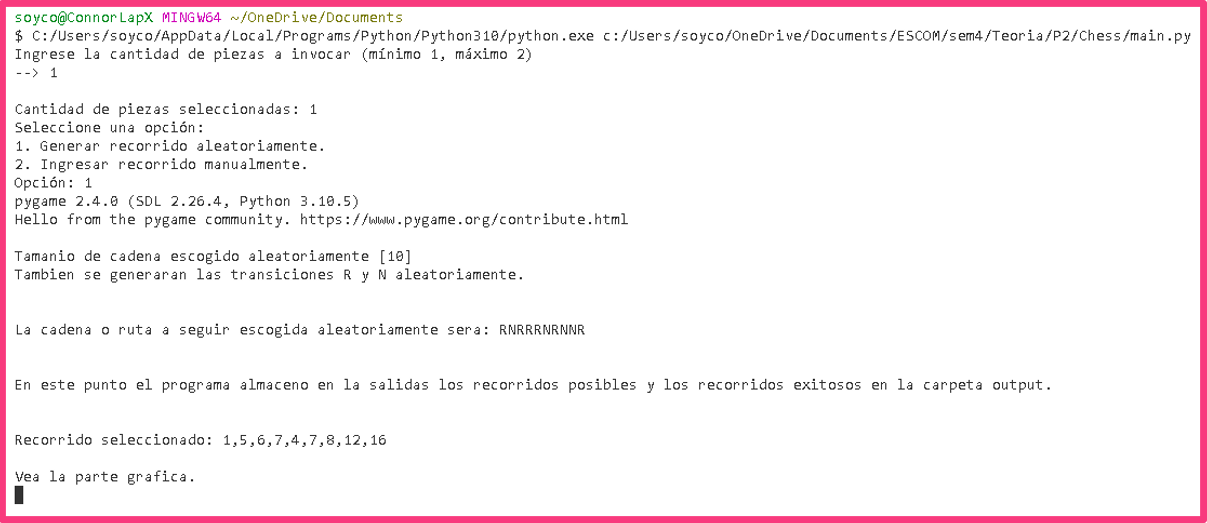
\includegraphics[width=4\linewidth]{Images/Cap1.png}
\end{minipage}
\caption{Inicio del programa en terminal.}
\label{fig:imagen}
\end{figure}
\newpage
\item Aquí podemos ver la salida del archivo recorrido\_blanca.txt y el de recorrido\_finales\_blanca.txt donde en el primero se almacenaron todos los recorridos posibles y en el segundo solo los recorridos que llevan al estado de éxito 16.  Observar la Figura 2.2.\newline
\begin{figure}[h]
%\begin{minipage}{0.3\textwidth}
    \begin{center}
    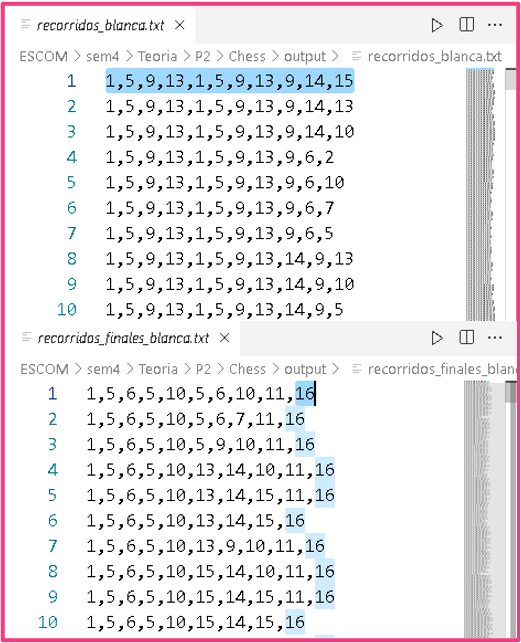
\includegraphics[width=0.7\linewidth]{Images/Cap6.png}
    \end{center}
%\end{minipage}
\caption{Vista de archivos de salida de recorridos.}
\label{fig:imagen}
\end{figure}

\newpage
\item Aquí se puede ver la secuencia que sigue la parte gráfica, donde al dar clic al botón $"$Siguiente$"$ nos lleva al siguiente movimiento. Observar la Figura 2.3.
\begin{figure}[h]
%\begin{minipage}{0.3\textwidth}
    \begin{center}
    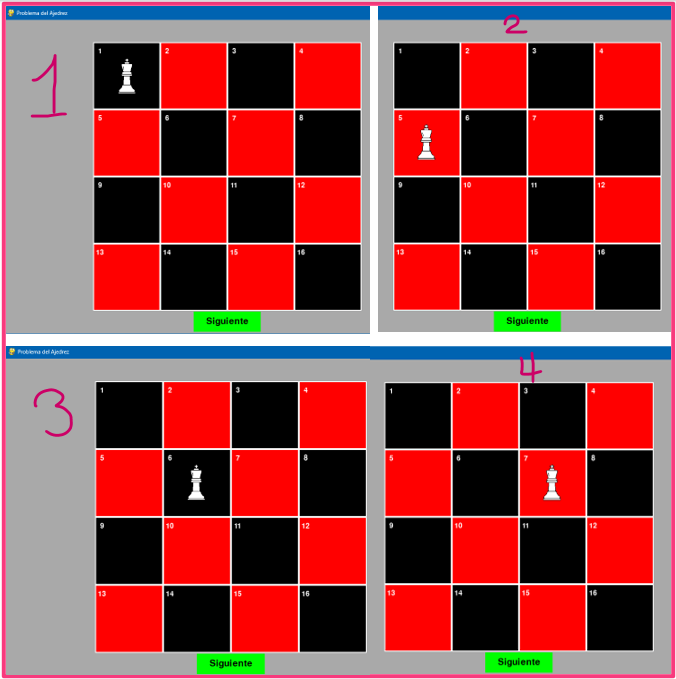
\includegraphics[width=0.8\linewidth]{Images/Cap2.png}
    \end{center}
%\end{minipage}
\caption{Visualización de transiciones gráficas.}
\label{fig:imagen}
\end{figure}

\newpage
\item Siguiente imagen de transiciones graficas. Observar la Figura 2.4.
\begin{figure}[h]
%\begin{minipage}{0.3\textwidth}
    \begin{center}
    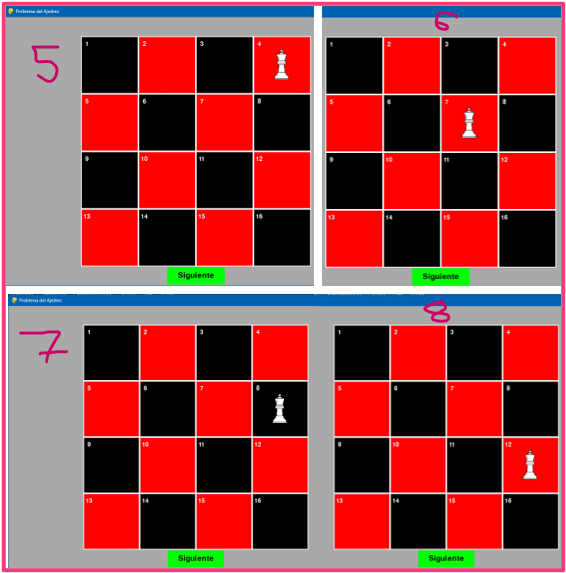
\includegraphics[width=0.7\linewidth]{Images/Cap3.png}
    \end{center}
%\end{minipage}
\caption{Transiciones graficas.}
\label{fig:imagen}
\end{figure}

\newpage
\item Final de la transición gráfica, el programa nos dice que ha terminado. Observar la figura 2.5.

\begin{figure}[h]
%\begin{minipage}{0.3\textwidth}
    \begin{center}
    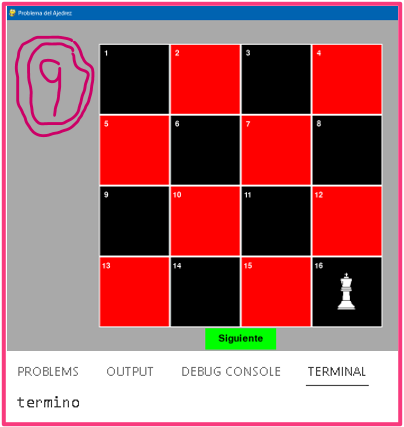
\includegraphics[width=0.7\linewidth]{Images/Cap4.png}
    \end{center}
%\end{minipage}
\caption{Fin de transición y final en terminal.}
\label{fig:imagen}
\end{figure}

\newpage
\item Aquí podemos ver el árbol de recorridos correspondiente al recorrido que se ha escogido aleatoriamente. Observar la figura 2.6.

\begin{figure}[h]
%\begin{minipage}{0.3\textwidth}
    \begin{center}
    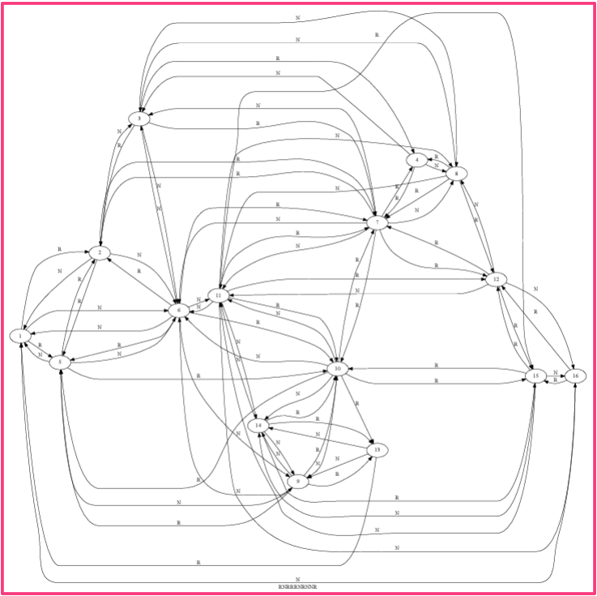
\includegraphics[width=0.7\linewidth]{Images/Cap5.png}
    \end{center}
%\end{minipage}
\caption{Grafo de recorrido.}
\label{fig:imagen}
\end{figure}
\newpage
\item Iniciamos el programa´nuevamente, donde nos pide que introduzcamos la cantidad de piezas a invocar en el tablero. Para este caso en particular se seleccionó 2 piezas. Ahora nos pide que elegíamos entre diferentes configuraciones, elegimos el caso de manual vs manual, que básicamente nosotros introduciremos el recorrido a recorrer. Luego nos muestra datos sobre las rutas seleccionadas aleatoriamente, su respectivo tamaño. Finalmente, nos indica que pieza empieza primero. Podemos observar que la pieza negra colisionará con la pieza blanca cuando esta se recorra al estado 6. Observar la figura 2.7.

\begin{figure}[h]
%\begin{minipage}{0.3\textwidth}
    \begin{center}
    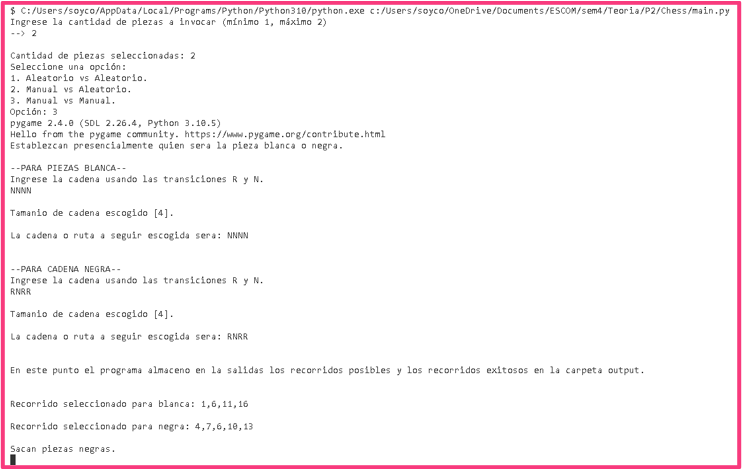
\includegraphics[width=0.8\linewidth]{Images/Cap7.png}
    \end{center}
%\end{minipage}
\caption{Vista de terminal de segundo caso.}
\label{fig:imagen}
\end{figure}
\newpage
\item Pasos de transiciones de la parte gráfica, donde en el último caso de transición se detecta la colisión y se recalcula una ruta. Observar figura 2.8.

\begin{figure}[h]
%\begin{minipage}{0.3\textwidth}
    \begin{center}
    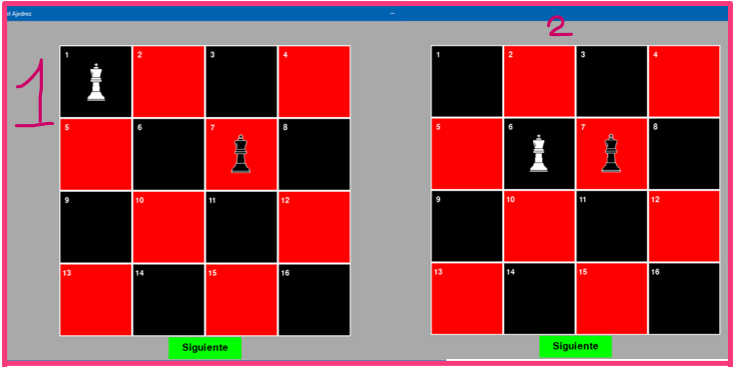
\includegraphics[width=0.8\linewidth]{Images/Cap9.png}
    \end{center}
%\end{minipage}
\caption{Secuencia de transiciones, donde en caso 2 hay colisión.}
\label{fig:imagen}
\end{figure}

\newpage
\item Se detecta una colisión, por ende se reconfigura el recorrido y por ende los recorridos posibles y los recorridos finales, por lo que se vuelve a escoger una ruta adecuada. Observar figura 2.9.

\begin{figure}[h]
%\begin{minipage}{0.3\textwidth}
    \begin{center}
    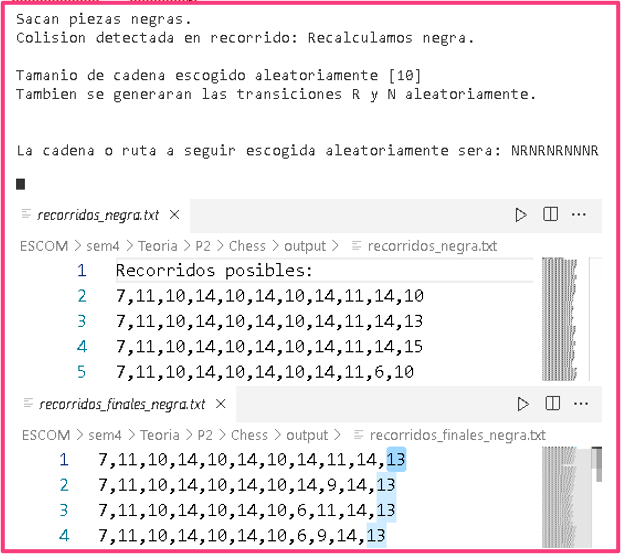
\includegraphics[width=0.8\linewidth]{Images/Cap10.png}
    \end{center}
%\end{minipage}
\caption{Vista de terminal de nueva ruta configurada y salida en archivos.}
\label{fig:imagen}
\end{figure}

\newpage
\item Regresamos a la parte gráfica donde ahora si nos reconfiguró una ruta para la pieza negra, donde podemos ver que la pieza blanca terminó por llegar primero al estado 16 y el juego se acaba. Observar figura 2.10.

\begin{figure}[h]
%\begin{minipage}{0.3\textwidth}
    \begin{center}
    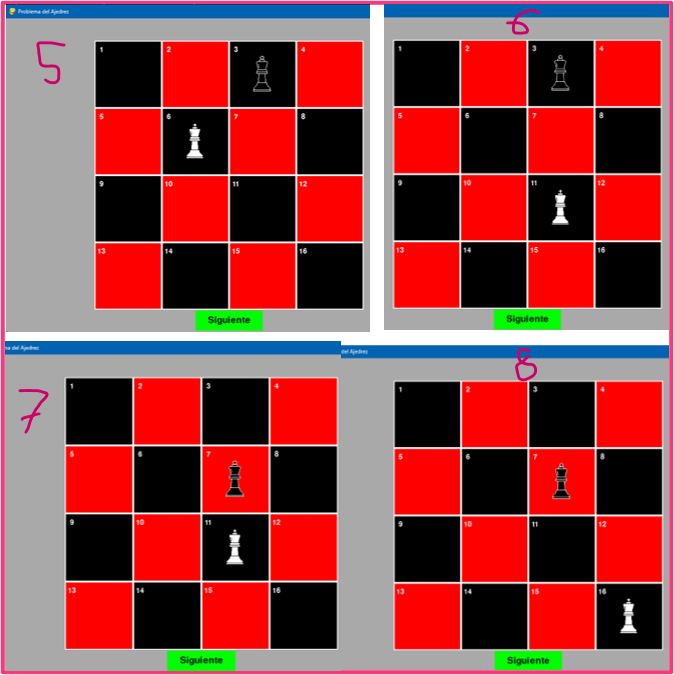
\includegraphics[width=0.8\linewidth]{Images/Cap11.png}
    \end{center}
%\end{minipage}
\caption{Vista de gráfica del ajedrez.}
\label{fig:imagen}
\end{figure}

\newpage
\item Aquí podemos ver la renderización del arbol o grafo de recorridos para pieza blanca.  Observar la figura 2.11.

\begin{figure}[h]
\begin{minipage}{0.3\textwidth}
    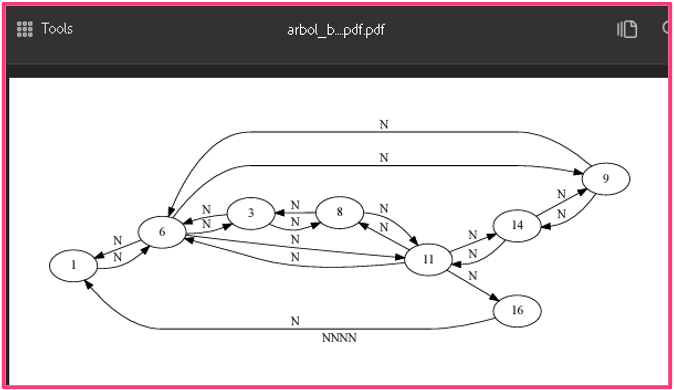
\includegraphics[width=4\linewidth]{Images/Cap12.png}
\end{minipage}
\caption{Árbol de recorridos para pieza blanca.}
\label{fig:imagen}
\end{figure}

\newpage
\item Aquí podemos ver la renderización del arbol o grafo de recorridos para pieza negra. Observar la figura 2.12.

\begin{figure}[h]
\begin{minipage}{0.3\textwidth}
    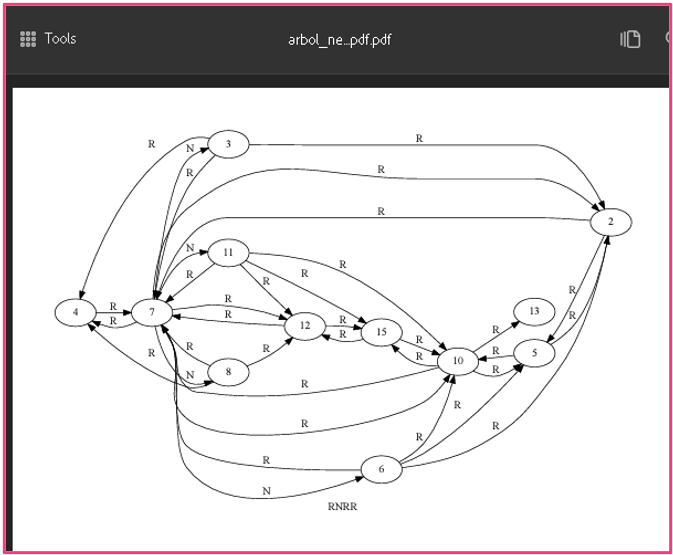
\includegraphics[width=4\linewidth]{Images/Cap13.png}
\end{minipage}
\caption{Árbol de recorridos para pieza negra.}
\label{fig:imagen}
\end{figure}
\newpage
\item Aquí podemos ver el caso para cuando digitamos un recorrido de mayor longitud, para este caso fue una cadena de recorrido de tamaño 82. Observar la figura 2.12.

\begin{figure}[h]
\begin{minipage}{0.3\textwidth}
    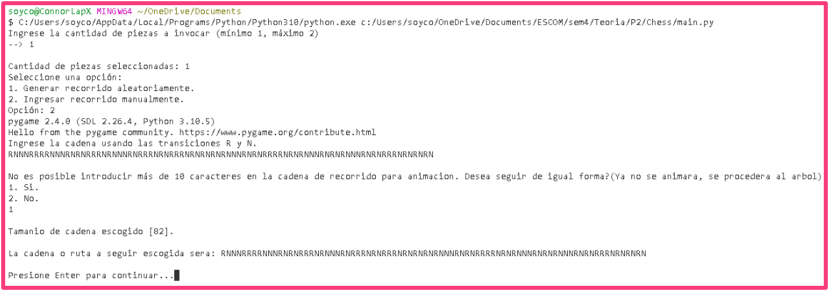
\includegraphics[width=4\linewidth]{Images/Cap14.png}
\end{minipage}
\caption{Vista de terminal para recorrido de tamaño 82.}
\label{fig:imagen}
\end{figure}
\newpage
\item Aquí podemos ver el archivo de recorridos posibles para la pieza, donde el formato de guardado del recorrido se almacena de manera muy distinta, siendo separado cada recorrido por puntos en vez de saltos de línea, para de esta manera evitar una creciente exponencial en la generación del documento. Observar la figura 2.12.

\begin{figure}[h]
\begin{minipage}{0.3\textwidth}
    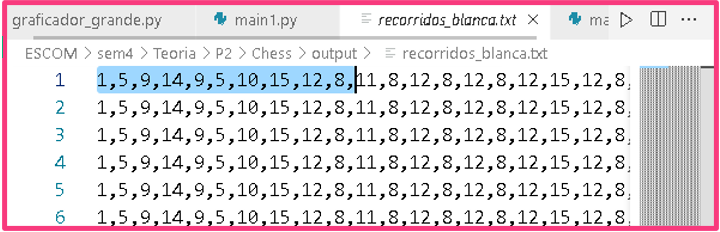
\includegraphics[width=4\linewidth]{Images/Cap15.png}
\end{minipage}
\caption{Vista de archivo de recorridos para la pieza blanca.}
\label{fig:imagen}
\end{figure}
\newpage
\item Grafo de recorridos para la cadena de tamaño 82. Observar la figura 2.12.

\begin{figure}[h]
\begin{minipage}{0.3\textwidth}
    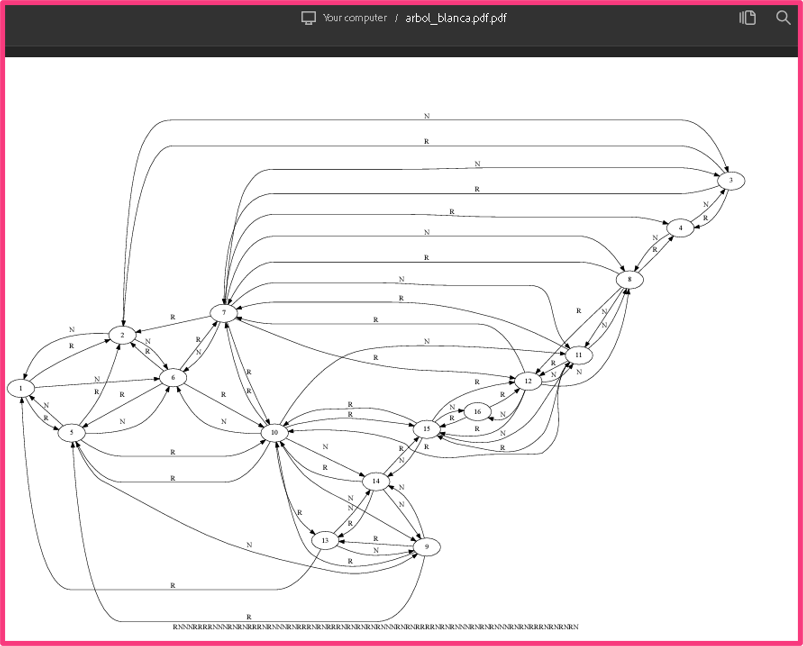
\includegraphics[width=4\linewidth]{Images/Cap16.png}
\end{minipage}
\caption{Árbol de recorridos para pieza en cuestión.}
\label{fig:imagen}
\end{figure}

\end{enumerate}
\chapter{Conclusión}

En primer lugar, he aprendido la importancia de la planificación y el diseño adecuado antes de comenzar a implementar una solución. Al enfrentar el desafío de representar un tablero de ajedrez en código, me di cuenta de que debía considerar cuidadosamente la estructura de datos y la forma en que se organizarían las piezas. Esto me enseñó a pensar en forma modular y a descomponer problemas complejos en partes más pequeñas y manejables.\newline

Además, esta práctica me brindó una oportunidad valiosa para aplicar mis conocimientos de programación orientada a objetos (POO). Pude utilizar clases y objetos para representar las piezas de ajedrez y manipular sus atributos y comportamientos. A través de esta experiencia, comprendí mejor los conceptos fundamentales de la POO, como la encapsulación, la herencia y el polimorfismo.\newline

También aprendí sobre la importancia de la abstracción y la claridad en el código. Al escribir el programa, me esforcé por utilizar nombres de variables y métodos descriptivos, lo que facilitó la comprensión y el mantenimiento del código en el futuro. Además, traté de evitar la duplicación de código y promoví la reutilización a través de la creación de funciones y métodos reutilizables.\newline

Otra conclusión clave es el valor de las pruebas y la depuración. Durante el proceso de desarrollo, me encontré con algunos errores y comportamientos inesperados. Aprendí a utilizar técnicas de depuración, como la impresión de mensajes y la revisión del flujo de ejecución, para identificar y corregir estos problemas. También descubrí la importancia de escribir pruebas unitarias para validar el funcionamiento de mi código y garantizar su correcta ejecución en diferentes escenarios.\newline

Por último, esta práctica me recordó la importancia de la paciencia y la perseverancia al enfrentar desafíos de programación. Hubo momentos en los que me sentí frustrado y bloqueado, pero aprendí a tomar descansos, buscar ayuda cuando fuera necesario y abordar los problemas paso a paso. Esto me enseñó a ser más resiliente y a mantener una mentalidad de resolución de problemas.\newline

Probé mi solución en varios casos de prueba y obtuvimos resultados precisos y eficientes. Sin embargo, también noté que la complejidad temporal de mi solución puede aumentar considerablemente en laberintos grandes con muchas palabras objetivo. En futuros trabajos, podría explorar otras técnicas de búsqueda que puedan ser más eficientes en casos de laberintos grandes y complejos.\newline
\\

\section{Problemas iniciales}
Durante la resolución de esta práctica del tablero de ajedrez, me encontré con varios problemas iniciales que debieron ser abordados para lograr una solución completa.\newline

En primer lugar, tuve que definir la estructura y el diseño del programa, decidiendo cómo organizar el código en archivos separados y estableciendo la interacción con el usuario a través de menús. Esto implicó considerar cómo generar y mostrar los recorridos de las piezas.\newline

Otro desafío importante fue la generación de los recorridos en sí. Cada pieza tiene reglas de movimiento específicas, por lo que fue necesario desarrollar algoritmos precisos y eficientes que tuvieran en cuenta posibles casos especiales, como los límites del tablero y la colisión con otras piezas.\newline

Una vez generados los recorridos, fue crucial validar su validez. Esto significaba asegurarse de que las piezas no se salieran del tablero y que no se superpusieran entre sí. Para lograr esto, implementé una lógica adicional para verificar cada movimiento y descartar los recorridos inválidos.\newline

Además, era importante representar visualmente los recorridos en el tablero de ajedrez. Esto requirió el uso de bibliotecas gráficas y la definición de la lógica para dibujar las piezas y las rutas de movimiento en la interfaz gráfica.\newline

Por último, consideré la eficiencia y el rendimiento del programa. Algunos recorridos, como los mayores a 10, crecían exponencialmente, lo que generaba inconvenientes adversos.\newline

\subsection{Soluciones}
A continuación, se detallan las soluciones que se les dieron a dichos problemas:
\begin{enumerate}
    \item Estructura y diseño del programa: Se optó por organizar el código en archivos separados para mejorar la modularidad y la legibilidad. Se crearon funciones de menú para interactuar con el usuario y seleccionar la cantidad de piezas y el tipo de recorrido. Además, se utilizó un enfoque basado en subprocessos para invocar los diferentes archivos Python según las selecciones del usuario.\newline 

    \item Generación de recorridos: Se implementaron algoritmos específicos para cada tipo de pieza (blanca y negra) que tuvieron en cuenta las reglas de movimiento de cada una. Se consideraron casos especiales, como la colisión con otras piezas, para generar recorridos válidos.\newline 
    
    \item Validación de recorridos: Se agregó lógica adicional para verificar la validez de los recorridos generados. En caso de detectar movimientos inválidos, se descartaron o ajustaron los recorridos correspondientes.\newline 
    
    \item Representación gráfica: Se utilizó una biblioteca gráfica, como Pygame, para mostrar visualmente los recorridos en el tablero de ajedrez. Se definió la lógica para dibujar las piezas y las rutas de movimiento en la interfaz gráfica, lo que permitió una representación clara y comprensible de los recorridos generados.\newline 
    
    \item Rendimiento y eficiencia: Se optimizó el código y los algoritmos para mejorar el rendimiento del programa, especialmente en casos donde las piezas tenían un gran número de movimientos posibles, como los recorridos mayores a 10, donde la solución fue un correcto almacenamiento de los recorridos y también su lectura. Se utilizaron técnicas de programación eficiente y se realizaron ajustes para evitar demoras excesivas en la generación y visualización de los recorridos.\newline 
\end{enumerate}
 \newline 
\section{Complejidades}
El algoritmo también incluye una función llamada $"$recorrer\_estados$"$ que genera todos los recorridos posibles en el juego del ajedrez. Esta función utiliza recursión para obtener los recorridos y es difícil determinar su complejidad exacta sin conocer la longitud máxima de los recorridos y el número de estados posibles. En el peor de los casos, la complejidad podría ser exponencial.\newline

En cuanto a la función $"$seleccionar\_recorrido$"$, selecciona una línea aleatoria de un archivo que contiene los recorridos finales válidos. La complejidad de esta función depende del tamaño del archivo y es lineal en función del número de líneas en el archivo.\newline

Básicamente, la complejidad del algoritmo del tablero de la práctica puede variar dependiendo de los detalles específicos y la longitud de los recorridos en el juego del ajedrez, sobretodo para recorridos como los mayores a 10, que crecen de manera exponencial.\newline
\chapter{Bibliografias}
\begin{enumerate}
    \item Salamanca, S., & García, J. (2019). Estrategias de juego y resolución de problemas en el ajedrez. Revista Internacional de Ajedrez y Educación, 42(2), 78-92.\newline
    \item Johnson, M. (2020). The Art of Chess: Tactics and Problem Solving. New York: Chess Publishing.\newline
    \item Williams, D. (2018). Mastering Chess: The Guide to Chess Tactics, Chess Openings, and Chess Strategies. New York: New Chess Press.\newline
    \item Sánchez, L. M. (2017). El tablero de ajedrez como herramienta para el desarrollo del pensamiento lógico-matemático. Revista de Investigación en Educación Matemática, 9(2), 145-160.\newline
\end{enumerate}















%\textbf{Nota}: {\color{red}Revisar esta sugerencia de Segun:} %\href{https://github.com/INGEOTEC/RegionalEmbeddings}{FastText Word Embeddings for Spanish Language Variations} 


%[Objetivo: ]

\chapter{Anexos}
\lstset{
    language=C,
    basicstyle=\ttfamily\small\color{black},
    numbers=left,
    numberstyle=\tiny,
    stepnumber=1,
    numbersep=8pt,
    backgroundcolor=\color{white},
    showspaces=false,
    showstringspaces=false,
    showtabs=false,
    frame=single,
    rulecolor=\color{magenta},
    tabsize=2,
    captionpos=b,
    breaklines=true,
    breakatwhitespace=false,
    title=\lstname,
    escapeinside={\%*}{*)},
    keywordstyle=\color{blue},
    commentstyle=\color{red},
    stringstyle=\color{orange},
    morecomment=[l][\color{red}]{\#},
    otherkeywords={=,!,<,>,*,+,-,&,|,^,~},
    numbers=left,                   % Coloca los números de línea a la izquierda
    numberstyle=\tiny\color{black}, % Estilo de los números de línea
    stepnumber=1,    % Incremento en el que se muestran los números de línea
    numbersep=8pt
}
\section{LATEX de exte proyecto}
Dirección Overleaf: \url{https://www.overleaf.com/3411646862zgynbbsnckcd}\newline
Dirección GitHub: \url{}\newline

\section{Main.py}
El código main solo es el programa principal que nos redireccionara a los archivos .py correspondientes a su asignmación. \newline
\\
\begin{lstlisting}
#Teoria de la computacion
#Buscador de palabras
#Alumno: Connor Urbano Mendoza
import os
import subprocess

def menu_piezas():
    cantidad = int(input("Ingrese la cantidad de piezas a invocar (mínimo 1, máximo 2)\n--> "))
    if cantidad < 1 or cantidad > 2:
        print("\nCantidad inválida. Por favor, ingrese 1 o 2.")
        return menu_piezas()  # Llamada recursiva si la cantidad es inválida
    else:
        return cantidad

def menu_recorrido(cantidad_piezas):
    #config==1 es para recorrido aleatorio
    #config==2 es para recorido manual
    if cantidad_piezas==1:
        #1 pieza
        opcion = int(input("Seleccione una opción:\n1. Generar recorrido aleatoriamente.\n2. Ingresar recorrido manualmente.\nOpción: "))
        if opcion == 1:
            return 1  # Opción de generar recorrido aleatoriamente
        elif opcion == 2:
            return 2  # Opción de ingresar recorrido manualmente
        else:
            print("Opción inválida. Por favor, seleccione 1 o 2.")
            return menu_recorrido(cantidad_piezas)  # Llamada recursiva si la opción es inválida
    else:
        #2 piezas
        opcion = int(input("Seleccione una opción:\n1. Aleatorio vs Aleatorio.\n2. Manual vs Aleatorio.\n3. Manual vs Manual.\nOpción: "))
        if opcion == 1:
            return 3  # Opción de generar recorrido aleatoriamente vs aleatoriamente
        elif opcion == 2:
            return 4  # Opción de ingresar recorrido manualmente vs aleatoriamente
        elif opcion == 3:
            return 5  # Opción de ingresar recorrido manualmente vs manualmente
        else:
            print("Opción inválida. Por favor, seleccione 1, 2 o 3.")
            return menu_recorrido(cantidad_piezas)  # Llamada recursiva si la opción es inválida
    
#Main del ciclo del juego
# Obtener directorio actual
directorio_actual = os.path.dirname(os.path.abspath(__file__))
cantidad_piezas = menu_piezas()
print("\nCantidad de piezas seleccionadas:", cantidad_piezas)
config = menu_recorrido(cantidad_piezas)
x=0
#Posibles configuraciones: 1,2,3,4 o 5.
if config == 1:#A
    archivo_py = os.path.join(directorio_actual, "main1.py")
    resultado = subprocess.run(["python", archivo_py])
    os.system('cls' if os.name == 'nt' else 'clear')
    codigo_salida = resultado.returncode
    x=1
    #print(codigo_salida)
elif config == 2:#Manual
    archivo_py = os.path.join(directorio_actual, "main2.py")
    resultado = subprocess.run(["python", archivo_py])
    os.system('cls' if os.name == 'nt' else 'clear')
    codigo_salida = resultado.returncode
    x=1
    #print(codigo_salida)
elif config == 3:#AvsA
    archivo_py = os.path.join(directorio_actual, "main3.py")
    resultado =subprocess.run(["python", archivo_py])
    os.system('cls' if os.name == 'nt' else 'clear')
    codigo_salida = resultado.returncode
    x=2
    #print(codigo_salida)
elif config == 4:#ManualvsA
    archivo_py = os.path.join(directorio_actual, "main4.py")
    resultado =subprocess.run(["python", archivo_py])
    os.system('cls' if os.name == 'nt' else 'clear')
    codigo_salida = resultado.returncode
    x=2
    #print(codigo_salida)
elif config == 5:#ManualvsManual
    archivo_py = os.path.join(directorio_actual, "main5.py")
    resultado =subprocess.run(["python", archivo_py])
    os.system('cls' if os.name == 'nt' else 'clear')
    codigo_salida = resultado.returncode
    x=2
    #print(codigo_salida)

if codigo_salida == 3:
    archivo_py = os.path.join(directorio_actual, "graficador_grande.py")
    subprocess.run(["python", archivo_py,(str(x))])
else:
    archivo_py = os.path.join(directorio_actual, "graficador.py")
    subprocess.run(["python", archivo_py,(str(x))])
print("termino")
\end{lstlisting}

\section{Main1.py}
El código main solo es el programa principal que nos redireccionara a los archivos .py correspondientes a su asignmación. \newline
\\
\begin{lstlisting}
#Teoria de la computacion
#Buscador de palabras
#Alumno: Connor Urbano Mendoza

import random
import pygame
import random
import os

pygame.init() #Acceso al paquete pygame
#Ancho
WIDTH = 1000
#Altura
HEIGHT = 700
screen = pygame.display.set_mode((WIDTH,HEIGHT)) #Tamanio de ventana a imprimir
pygame.display.set_caption('Problema del Ajedrez')
font = pygame.font.Font('freesansbold.ttf',20)#Tipo de fuente 1 del juego
big_font= pygame.font.Font('freesansbold.ttf',50)#Tipo de fuente 2 del juego
timer = pygame.time.Clock()#velocidad de actualizacion de nuestro juego a 60 fps
fps=60

#NFA de estados
tablaEstados = {
    '1' : {'R': {'2','5'}, 'N': '6'},
    '2' : {'R': {'5','7'}, 'N': {'1','6','3'}},
    '3' : {'R': {'2','7','4'}, 'N': {'6','8'}},
    '4' : {'R': '7', 'N': {'3','8'}},
    '5' : {'R': {'2','10'}, 'N': {'1','6','9'}},
    '6' : {'R': {'2','5','7','10'}, 'N': {'1','3','9','11'}},
    '7' : {'R': {'2','4','10','12'}, 'N': {'3','6','8','11'}},
    '8' : {'R': {'4','7','12'}, 'N': {'3','11'}},
    '9' : {'R': {'5','10','13'}, 'N': {'6','14'}},
    '10' : {'R': {'5','7','13','15'}, 'N': {'6','9','11','14'}},
    '11' : {'R': {'7','10','12','15'}, 'N': {'6','8','14','16'}},
    '12' : {'R': {'7','15'}, 'N': {'8','11','16'}},
    '13' : {'R': '10', 'N': {'9','14'}},
    '14' : {'R': {'13','10','15'}, 'N': {'9','11'}},
    '15' : {'R': {'10','12'}, 'N': {'11','14','16'}},
    '16' : {'R': {'12','15'}, 'N': '11'}#Estado 16 es el estado Final.
}

#Variables e imagenes del juego
pieza_blanca = ['king']
posicion_blanca =[(235,85)]

#Variables de turnos cambiantes
turn_step = 0
selection= 100
#Cargar imagenes en juego
rey_blanco = pygame.image.load('C:\\Users\\soyco\\OneDrive\\Documents\\ESCOM\\sem4\\Teoria\\P2\\Chess\\img\\white_king.png')
rey_blanco = pygame.transform.scale(rey_blanco,(80,80))

imagen_blanca = [rey_blanco]

lista_piezas = ['king']

#ver variables/contador flash
boton_presionado = False

def dibujar_boton():
    boton_width = 150
    boton_height = 45
    boton_x = (WIDTH - boton_width) // 2
    boton_y = (HEIGHT - boton_height - 20)+17

    # Dibujar el botón como un rectángulo en la pantalla
    boton_rect=pygame.Rect(boton_x, boton_y, boton_width, boton_height)
    pygame.draw.rect(screen, (0, 255, 0), (boton_x, boton_y, boton_width, boton_height))
    texto = font.render("Siguiente", True, (0, 0, 0))
    texto_rect = texto.get_rect(center=(boton_x + boton_width // 2, boton_y + boton_height // 2))
    screen.blit(texto, texto_rect)
    return boton_rect
    
#Funcion para dibujar tablero
def dibujar_tablero():
    cuadro_size = 150  # Tamaño de cada cuadro del tablero
    tablero_width = 4 * cuadro_size  # Ancho total del tablero
    tablero_height = 4 * cuadro_size  # Altura total del tablero
    tablero_x = (WIDTH - tablero_width) // 2  # Posición X para centrar el tablero
    tablero_y = (HEIGHT - tablero_height) // 2  # Posición Y para centrar el tablero
    
    numero_color = 'white'  # Color del número de casilla

    font = pygame.font.Font(None, 24)  # Fuente y tamaño del número de casilla

    for i in range(16):  # Iterar 16 veces para un tablero de 4x4
        columna = i % 4
        fila = i // 4
        x = tablero_x + columna * cuadro_size
        y = tablero_y + fila * cuadro_size
        if fila % 2 == 0:
            color = 'black' if columna % 2 == 0 else 'red'
        else:
            color = 'red' if columna % 2 == 0 else 'black'
        pygame.draw.rect(screen, color, [x, y, cuadro_size, cuadro_size])
        pygame.draw.rect(screen, 'white', [x, y, cuadro_size, cuadro_size], 2)  # Agregar borde de color blanco
        numero_texto = font.render(str(i + 1), True, numero_color)  # Crear superficie de texto con el número
        numero_rect = numero_texto.get_rect(center=((x + cuadro_size // 2)-60, y + 20))  # Posición del número en la parte superior del recuadro
        screen.blit(numero_texto, numero_rect)  # Pegar el número en la pantalla

#Funcion para dibujar piezas
def dibujar_piezas():
    index=lista_piezas.index('king')
    if pieza_blanca[0]=='king':     
        
        screen.blit(imagen_blanca[index],(posicion_blanca[0][0],posicion_blanca[0][1]))
           
def recorrer_estados(tabla_estados, cadena):
    # Función para obtener todos los recorridos posibles
    def obtener_recorridos(estado_actual, simbolos_restantes, recorrido_actual):
        if not simbolos_restantes:
            recorridos.append(recorrido_actual)
            return

        simbolo = simbolos_restantes[0]
        if estado_actual in tabla_estados and simbolo in tabla_estados[estado_actual]:
            transiciones = tabla_estados[estado_actual][simbolo]

            for estado_siguiente in transiciones:
                obtener_recorridos(estado_siguiente, simbolos_restantes[1:], recorrido_actual + [estado_siguiente])

    # Función para obtener los recorridos válidos hasta el estado final
    def obtener_recorridos_finales(estado_actual, simbolos_restantes, recorrido_actual):
        if estado_actual == '16':
            recorridos_finales.append(recorrido_actual)
            return

        if not simbolos_restantes:
            return

        simbolo = simbolos_restantes[0]
        if estado_actual in tabla_estados and simbolo in tabla_estados[estado_actual]:
            transiciones = tabla_estados[estado_actual][simbolo]

            for estado_siguiente in transiciones:
                obtener_recorridos_finales(estado_siguiente, simbolos_restantes[1:], recorrido_actual + [estado_siguiente])

    # Obtener recorridos posibles
    recorridos = []
    obtener_recorridos('1', cadena, ['1'])

    # Obtener recorridos hasta el estado final
    recorridos_finales = []
    obtener_recorridos_finales('1', cadena, ['1'])

    # Guardar los recorridos en archivos de texto
    with open('C:\\Users\\soyco\\OneDrive\\Documents\\ESCOM\\sem4\\Teoria\\P2\\Chess\\output\\recorridos_blanca.txt', 'w') as archivo_recorridos:
        archivo_recorridos.write('Recorridos posibles:\n')
        for recorrido in recorridos:
            archivo_recorridos.write(','.join(recorrido) + '\n')

    with open('C:\\Users\\soyco\\OneDrive\\Documents\\ESCOM\\sem4\\Teoria\\P2\\Chess\\output\\recorridos_finales_blanca.txt', 'w') as archivo_recorridos_finales:
        for recorrido in recorridos_finales:
            archivo_recorridos_finales.write(','.join(recorrido) + '\n')



def seleccionar_recorrido():
    ruta_archivo = "C:\\Users\\soyco\\OneDrive\\Documents\\ESCOM\\sem4\\Teoria\\P2\\Chess\\output\\recorridos_finales_blanca.txt"
    
    with open(ruta_archivo, "r") as archivo:
        if os.path.getsize(ruta_archivo) == 0:
            print("No existen soluciones que lleguen al estado 16 con la condicion actual. Se recalculara una ruta.\n")
            nuevaruta=cadena()
            print("La nueva ruta es: "+nuevaruta)
            recorrer_estados(tablaEstados, nuevaruta)
            print('Se almacenaron las nuevas salidas de los recorridos posibles y los recorridos exitosos en la carpeta output.\n')
            
            return seleccionar_recorrido()
            
        lineas = archivo.readlines()
        
        # Seleccionar una línea aleatoria
        recorrido_seleccionado = random.choice(lineas)
        
        # Eliminar los espacios en blanco y saltos de línea
        recorrido_seleccionado = recorrido_seleccionado.strip()
        
        return recorrido_seleccionado

def cadenaRandom(numero): #Genera un string de forma random 
    auxiliar = '' #Variable auxiliar
    for i in range(numero):
        x = random.randint(1, 2) #Función para generar un resultado random de una lista
        if x % 2 == 0:
            auxiliar = auxiliar + "R"
        else:
            auxiliar = auxiliar + "N"
    return auxiliar

def cadena():
    numero = random.randint(4,10)
    print('\nTamanio de cadena escogido aleatoriamente ['+str(numero)+']\nTambien se generaran las transiciones R y N aleatoriamente.\n')
    cad = cadenaRandom(numero) #Se genera de forma aleatoria del 1-10
    print('\nLa cadena o ruta a seguir escogida aleatoriamente sera: '+cad+'\n')
    return cad

def calcular_coordenadas(estado):
    cuadro_size = 150  # Tamaño de cada cuadro del tablero
    tablero_width = 4 * cuadro_size  # Ancho total del tablero
    tablero_height = 4 * cuadro_size  # Altura total del tablero
    tablero_x = (WIDTH - tablero_width) // 2  # Posición X para centrar el tablero
    tablero_y = (HEIGHT - tablero_height) // 2  # Posición Y para centrar el tablero
    fila = (estado - 1) // 4  # Calcular la fila del estado
    columna = (estado - 1) % 4  # Calcular la columna del estado
    x = tablero_x + columna * cuadro_size  # Calcular la coordenada X del estado
    y = tablero_y + fila * cuadro_size  # Calcular la coordenada Y del estado
    return ((x+33), y+33)  # Devolver las coordenadas como una tupla


#Main del ciclo del juego 1
ruta=cadena()#Solicitamos la cadena generada aleatoriamente.
recorrer_estados(tablaEstados, ruta)
print('\nEn este punto el programa almaceno en la salidas los recorridos posibles y los recorridos exitosos en la carpeta output.\n')
recorrido = seleccionar_recorrido()#Este fue el recorrido que se escogio de manera aleatoria
with open('C:\\Users\\soyco\\OneDrive\\Documents\\ESCOM\\sem4\\Teoria\\P2\\Chess\\output\\ruta_blanca.txt', 'w') as archivo:
    archivo.write(ruta)
print("\nRecorrido seleccionado:", recorrido)
print("\nVea la parte grafica.")
lista_estados = [int(num) for num in recorrido.split(",")]

coordenadas=(235,85)
nueva_coordenada=(0,0)
run=True
contador=1
while run:
    timer.tick(fps)
    screen.fill('dark gray')
    dibujar_tablero()
    dibujar_piezas()
    boton_rect = dibujar_boton()

    for event in pygame.event.get():
        if event.type == pygame.QUIT:
            run = False

        if event.type == pygame.MOUSEBUTTONDOWN and event.button == 1:
            mouse_pos = pygame.mouse.get_pos()
            if boton_rect.collidepoint(mouse_pos):  # Verificar si se hizo clic en el botón
                
                nueva_coordenada = calcular_coordenadas(lista_estados[contador])
                
                if turn_step <= 1:
                    if coordenadas in posicion_blanca:
                        selection = posicion_blanca.index(coordenadas)
                        if turn_step == 0:
                            turn_step = 1
                        
                    if turn_step==1 and selection != 100:
                        posicion_blanca[0] = nueva_coordenada
                        
                        selection = 100
                        contador += 1
                        coordenadas = nueva_coordenada
                        turn_step=0

    pygame.display.flip()


pygame.quit()

\end{lstlisting}


\section{Main2.py}
El código main solo es el programa principal que nos redireccionara a los archivos .py correspondientes a su asignmación. \newline
\\
\begin{lstlisting}
#Teoria de la computacion
#Buscador de palabras
#Alumno: Connor Urbano Mendoza

import random
import pygame
import random
import os
import sys

pygame.init() #Acceso al paquete pygame
#Ancho
WIDTH = 1000
#Altura
HEIGHT = 700
screen = pygame.display.set_mode((WIDTH,HEIGHT)) #Tamanio de ventana a imprimir
pygame.display.set_caption('Problema del Ajedrez')
font = pygame.font.Font('freesansbold.ttf',20)#Tipo de fuente 1 del juego
big_font= pygame.font.Font('freesansbold.ttf',50)#Tipo de fuente 2 del juego
timer = pygame.time.Clock()#velocidad de actualizacion de nuestro juego a 60 fps
fps=60

#NFA de estados
tablaEstados = {
    '1' : {'R': {'2','5'}, 'N': '6'},
    '2' : {'R': {'5','7'}, 'N': {'1','6','3'}},
    '3' : {'R': {'2','7','4'}, 'N': {'6','8'}},
    '4' : {'R': '7', 'N': {'3','8'}},
    '5' : {'R': {'2','10'}, 'N': {'1','6','9'}},
    '6' : {'R': {'2','5','7','10'}, 'N': {'1','3','9','11'}},
    '7' : {'R': {'2','4','10','12'}, 'N': {'3','6','8','11'}},
    '8' : {'R': {'4','7','12'}, 'N': {'3','11'}},
    '9' : {'R': {'5','10','13'}, 'N': {'6','14'}},
    '10' : {'R': {'5','7','13','15'}, 'N': {'6','9','11','14'}},
    '11' : {'R': {'7','10','12','15'}, 'N': {'6','8','14','16'}},
    '12' : {'R': {'7','15'}, 'N': {'8','11','16'}},
    '13' : {'R': '10', 'N': {'9','14'}},
    '14' : {'R': {'13','10','15'}, 'N': {'9','11'}},
    '15' : {'R': {'10','12'}, 'N': {'11','14','16'}},
    '16' : {'R': {'12','15'}, 'N': '11'}#Estado 16 es el estado Final.
}

#Variables e imagenes del juego
pieza_blanca = ['king']
posicion_blanca =[(235,85)]

#
turn_step = 0
selection= 100
#Cargar imagenes en juego
rey_blanco = pygame.image.load('C:\\Users\\soyco\\OneDrive\\Documents\\ESCOM\\sem4\\Teoria\\P2\\Chess\\img\\white_king.png')
rey_blanco = pygame.transform.scale(rey_blanco,(80,80))

imagen_blanca = [rey_blanco]

lista_piezas = ['king']
#ver variables/contador flash


boton_presionado = False

def dibujar_boton():
    boton_width = 150
    boton_height = 45
    boton_x = (WIDTH - boton_width) // 2
    boton_y = (HEIGHT - boton_height - 20)+17

    # Dibujar el botón como un rectángulo en la pantalla
    boton_rect=pygame.Rect(boton_x, boton_y, boton_width, boton_height)
    pygame.draw.rect(screen, (0, 255, 0), (boton_x, boton_y, boton_width, boton_height))
    texto = font.render("Siguiente", True, (0, 0, 0))
    texto_rect = texto.get_rect(center=(boton_x + boton_width // 2, boton_y + boton_height // 2))
    screen.blit(texto, texto_rect)
    return boton_rect
    
#Funcion para dibujar tablero
def dibujar_tablero():
    cuadro_size = 150  # Tamaño de cada cuadro del tablero
    tablero_width = 4 * cuadro_size  # Ancho total del tablero
    tablero_height = 4 * cuadro_size  # Altura total del tablero
    tablero_x = (WIDTH - tablero_width) // 2  # Posición X para centrar el tablero
    tablero_y = (HEIGHT - tablero_height) // 2  # Posición Y para centrar el tablero
    
    numero_color = 'white'  # Color del número de casilla

    font = pygame.font.Font(None, 24)  # Fuente y tamaño del número de casilla

    for i in range(16):  # Iterar 16 veces para un tablero de 4x4
        columna = i % 4
        fila = i // 4
        x = tablero_x + columna * cuadro_size
        y = tablero_y + fila * cuadro_size
        if fila % 2 == 0:
            color = 'black' if columna % 2 == 0 else 'red'
        else:
            color = 'red' if columna % 2 == 0 else 'black'
        pygame.draw.rect(screen, color, [x, y, cuadro_size, cuadro_size])
        pygame.draw.rect(screen, 'white', [x, y, cuadro_size, cuadro_size], 2)  # Agregar borde de color blanco
        numero_texto = font.render(str(i + 1), True, numero_color)  # Crear superficie de texto con el número
        numero_rect = numero_texto.get_rect(center=((x + cuadro_size // 2)-60, y + 20))  # Posición del número en la parte superior del recuadro
        screen.blit(numero_texto, numero_rect)  # Pegar el número en la pantalla

#Funcion para dibujar piezas
def dibujar_piezas():
    index=lista_piezas.index('king')
    if pieza_blanca[0]=='king':     
        
        screen.blit(imagen_blanca[index],(posicion_blanca[0][0],posicion_blanca[0][1]))
  
def recorrer_estados(tabla_estados, cadena):
    
    # Función para obtener todos los recorridos posibles
    def obtener_recorridos(estado_actual, simbolos_restantes, recorrido_actual, archivo_recorridos):
        if not simbolos_restantes:
            archivo_recorridos.write(','.join(recorrido_actual) + '\n')
            return

        simbolo = simbolos_restantes[0]
        if estado_actual in tabla_estados and simbolo in tabla_estados[estado_actual]:
            transiciones = tabla_estados[estado_actual][simbolo]

            for estado_siguiente in transiciones:
                obtener_recorridos(
                    estado_siguiente,
                    simbolos_restantes[1:],
                    recorrido_actual + [estado_siguiente],
                    archivo_recorridos
                )

    # Función para obtener los recorridos válidos hasta el estado final
    def obtener_recorridos_finales(estado_actual, simbolos_restantes, recorrido_actual, archivo_recorridos_finales):
        if estado_actual == '16':
            archivo_recorridos_finales.write(','.join(recorrido_actual) + '\n')
            return

        if not simbolos_restantes:
            return

        simbolo = simbolos_restantes[0]
        if estado_actual in tabla_estados and simbolo in tabla_estados[estado_actual]:
            transiciones = tabla_estados[estado_actual][simbolo]

            for estado_siguiente in transiciones:
                obtener_recorridos_finales(
                    estado_siguiente,
                    simbolos_restantes[1:],
                    recorrido_actual + [estado_siguiente],
                    archivo_recorridos_finales
                )

    # Obtener recorridos posibles
    with open('C:\\Users\\soyco\\OneDrive\\Documents\\ESCOM\\sem4\\Teoria\\P2\\Chess\\output\\recorridos_blanca.txt', 'w') as archivo_recorridos:
        obtener_recorridos('1', cadena, ['1'], archivo_recorridos)

    # Obtener recorridos hasta el estado final
    with open('C:\\Users\\soyco\\OneDrive\\Documents\\ESCOM\\sem4\\Teoria\\P2\\Chess\\output\\recorridos_finales_blanca.txt', 'w') as archivo_recorridos_finales:
        obtener_recorridos_finales('1', cadena, ['1'], archivo_recorridos_finales)


def seleccionar_recorrido():
    ruta_archivo = "C:\\Users\\soyco\\OneDrive\\Documents\\ESCOM\\sem4\\Teoria\\P2\\Chess\\output\\recorridos_finales_blanca.txt"
    
    with open(ruta_archivo, "r") as archivo:
        if os.path.getsize(ruta_archivo) == 0:
            print("No existen soluciones que lleguen al estado 16 con la condicion actual. Ingrese nueva ruta.")
            nuevaruta=cadena()
            print("La nueva ruta es: "+nuevaruta)
            recorrer_estados(tablaEstados, nuevaruta)
            print('Se almacenaron las nuevas salidas de los recorridos posibles y los recorridos exitosos en la carpeta output.\n')
            lineas = archivo.readlines()
            # Seleccionar una línea aleatoria
            recorrido_seleccionado = random.choice(lineas)
            
            # Eliminar los espacios en blanco y saltos de línea
            recorrido_seleccionado = recorrido_seleccionado.strip()
            
            return recorrido_seleccionado
        
            
        lineas = archivo.readlines()
        
        # Seleccionar una línea aleatoria
        recorrido_seleccionado = random.choice(lineas)
        
        # Eliminar los espacios en blanco y saltos de línea
        recorrido_seleccionado = recorrido_seleccionado.strip()
        
        return recorrido_seleccionado

def cadena():
    while 1:
        ruta = input("Ingrese la cadena usando las transiciones R y N.\n").upper()
        if len(ruta) > 10:
            print("\nNo es posible introducir más de 10 caracteres en la cadena de recorrido para animacion. Desea seguir de igual forma?(Ya no se animara, se procedera al arbol)")
            respuesta = int(input("1. Si.\n2. No.\n"))
            if respuesta == 1:
                break
            else:
                pass
        else:
            print()
            break
    print('\nTamanio de cadena escogido ['+str(len(ruta))+'].')
    print('\nLa cadena o ruta a seguir escogida sera: '+ruta+'\n')
    return ruta

def calcular_coordenadas(estado):
    cuadro_size = 150  # Tamaño de cada cuadro del tablero
    tablero_width = 4 * cuadro_size  # Ancho total del tablero
    tablero_height = 4 * cuadro_size  # Altura total del tablero
    tablero_x = (WIDTH - tablero_width) // 2  # Posición X para centrar el tablero
    tablero_y = (HEIGHT - tablero_height) // 2  # Posición Y para centrar el tablero
    fila = (estado - 1) // 4  # Calcular la fila del estado
    columna = (estado - 1) % 4  # Calcular la columna del estado
    x = tablero_x + columna * cuadro_size  # Calcular la coordenada X del estado
    y = tablero_y + fila * cuadro_size  # Calcular la coordenada Y del estado
    
    return ((x+33), y+33)  # Devolver las coordenadas como una tupla



#Main del ciclo del juego 2
ruta=cadena()#Solicitamos la cadena generada aleatoriamente.
with open('C:\\Users\\soyco\\OneDrive\\Documents\\ESCOM\\sem4\\Teoria\\P2\\Chess\\output\\ruta_blanca.txt', 'w') as archivo:
    archivo.write(ruta)
if len(ruta)> 10:
    input("Presione Enter para continuar...")
    sys.exit(3)    
recorrer_estados(tablaEstados, ruta)
print('\nEn este punto el programa almaceno en la salidas los recorridos posibles y los recorridos exitosos en la carpeta output.\n')
recorrido = seleccionar_recorrido()#Este fue el recorrido que se escogio de manera aleatoria

with open('C:\\Users\\soyco\\OneDrive\\Documents\\ESCOM\\sem4\\Teoria\\P2\\Chess\\output\\ruta_blanca.txt', 'w') as archivo:
    archivo.write(ruta)

print("\nRecorrido seleccionado:", recorrido)
print("\nVea la parte grafica.")
lista_estados = [int(num) for num in recorrido.split(",")]

coordenadas=(235,85)
nueva_coordenada=(0,0)
run=True
contador=1
while run:
    timer.tick(fps)
    screen.fill('dark gray')
    dibujar_tablero()
    dibujar_piezas()
    boton_rect = dibujar_boton()

    for event in pygame.event.get():
        if event.type == pygame.QUIT:
            run = False

        if event.type == pygame.MOUSEBUTTONDOWN and event.button == 1:
            mouse_pos = pygame.mouse.get_pos()
            if boton_rect.collidepoint(mouse_pos):  # Verificar si se hizo clic en el botón
                
                nueva_coordenada = calcular_coordenadas(lista_estados[contador])
                
                if turn_step <= 1:
                    if coordenadas in posicion_blanca:
                        selection = posicion_blanca.index(coordenadas)
                        if turn_step == 0:
                            turn_step = 1
                        
                    if turn_step==1 and selection != 100:
                        posicion_blanca[0] = nueva_coordenada
                        selection = 100
                        contador += 1
                        coordenadas = nueva_coordenada
                        turn_step=0

    pygame.display.flip()


pygame.quit()

\end{lstlisting}


\section{Main3.py}
El código main solo es el programa principal que nos redireccionara a los archivos .py correspondientes a su asignmación. \newline
\\
\begin{lstlisting}
#Teoria de la computacion
#Buscador de palabras
#Alumno: Connor Urbano Mendoza

import random
import pygame
import random
import os

pygame.init() #Acceso al paquete pygame
#Ancho
WIDTH = 1000
#Altura
HEIGHT = 700
screen = pygame.display.set_mode((WIDTH,HEIGHT)) #Tamanio de ventana a imprimir
pygame.display.set_caption('Problema del Ajedrez')
font = pygame.font.Font('freesansbold.ttf',20)#Tipo de fuente 1 del juego
big_font= pygame.font.Font('freesansbold.ttf',50)#Tipo de fuente 2 del juego
timer = pygame.time.Clock()#velocidad de actualizacion de nuestro juego a 60 fps
fps=60

#NFA de estados
tablaEstados = {
    '1' : {'R': {'2','5'}, 'N': '6'},
    '2' : {'R': {'5','7'}, 'N': {'1','6','3'}},
    '3' : {'R': {'2','7','4'}, 'N': {'6','8'}},
    '4' : {'R': '7', 'N': {'3','8'}},
    '5' : {'R': {'2','10'}, 'N': {'1','6','9'}},
    '6' : {'R': {'2','5','7','10'}, 'N': {'1','3','9','11'}},
    '7' : {'R': {'2','4','10','12'}, 'N': {'3','6','8','11'}},
    '8' : {'R': {'4','7','12'}, 'N': {'3','11'}},
    '9' : {'R': {'5','10','13'}, 'N': {'6','14'}},
    '10' : {'R': {'5','7','13','15'}, 'N': {'6','9','11','14'}},
    '11' : {'R': {'7','10','12','15'}, 'N': {'6','8','14','16'}},
    '12' : {'R': {'7','15'}, 'N': {'8','11','16'}},
    '13' : {'R': '10', 'N': {'9','14'}},
    '14' : {'R': {'13','10','15'}, 'N': {'9','11'}},
    '15' : {'R': {'10','12'}, 'N': {'11','14','16'}},
    '16' : {'R': {'12','15'}, 'N': '11'}#Estado 16 es el estado Final.
}

#Variables e imagenes del juego
pieza_blanca = ['king']
pieza_negra = ['king']
posicion_blanca =[(235,85)]
posicion_negra =[(683,85)]

#
turn_step = 0
selection= 100
valid_moves_for1 =[]
#Cargar imagenes en juego
rey_blanco = pygame.image.load('C:\\Users\\soyco\\OneDrive\\Documents\\ESCOM\\sem4\\Teoria\\P2\\Chess\\img\\white_king.png')
rey_blanco = pygame.transform.scale(rey_blanco,(80,80))
rey_negro = pygame.image.load('C:\\Users\\soyco\\OneDrive\\Documents\\ESCOM\\sem4\\Teoria\\P2\\Chess\\img\\black_king.png')
rey_negro = pygame.transform.scale(rey_negro,(80,80))

imagen_blanca = [rey_blanco]
imagen_negra=[rey_negro]

lista_piezas = ['king']
#ver variables/contador flash


boton_presionado = False

def dibujar_boton():
    boton_width = 150
    boton_height = 45
    boton_x = (WIDTH - boton_width) // 2
    boton_y = (HEIGHT - boton_height - 20)+17

    # Dibujar el botón como un rectángulo en la pantalla
    boton_rect=pygame.Rect(boton_x, boton_y, boton_width, boton_height)
    pygame.draw.rect(screen, (0, 255, 0), (boton_x, boton_y, boton_width, boton_height))
    texto = font.render("Siguiente", True, (0, 0, 0))
    texto_rect = texto.get_rect(center=(boton_x + boton_width // 2, boton_y + boton_height // 2))
    screen.blit(texto, texto_rect)
    return boton_rect
    
#Funcion para dibujar tablero
def dibujar_tablero():
    cuadro_size = 150  # Tamaño de cada cuadro del tablero
    tablero_width = 4 * cuadro_size  # Ancho total del tablero
    tablero_height = 4 * cuadro_size  # Altura total del tablero
    tablero_x = (WIDTH - tablero_width) // 2  # Posición X para centrar el tablero
    tablero_y = (HEIGHT - tablero_height) // 2  # Posición Y para centrar el tablero
    
    numero_color = 'white'  # Color del número de casilla

    font = pygame.font.Font(None, 24)  # Fuente y tamaño del número de casilla

    for i in range(16):  # Iterar 16 veces para un tablero de 4x4
        columna = i % 4
        fila = i // 4
        x = tablero_x + columna * cuadro_size
        y = tablero_y + fila * cuadro_size
        if fila % 2 == 0:
            color = 'black' if columna % 2 == 0 else 'red'
        else:
            color = 'red' if columna % 2 == 0 else 'black'
        pygame.draw.rect(screen, color, [x, y, cuadro_size, cuadro_size])
        pygame.draw.rect(screen, 'white', [x, y, cuadro_size, cuadro_size], 2)  # Agregar borde de color blanco
        numero_texto = font.render(str(i + 1), True, numero_color)  # Crear superficie de texto con el número
        numero_rect = numero_texto.get_rect(center=((x + cuadro_size // 2)-60, y + 20))  # Posición del número en la parte superior del recuadro
        screen.blit(numero_texto, numero_rect)  # Pegar el número en la pantalla

#Funcion para dibujar piezas
def dibujar_piezas():
    index=lista_piezas.index('king')
    if pieza_blanca[0]=='king':     
        screen.blit(imagen_blanca[index],(posicion_blanca[0][0],posicion_blanca[0][1]))
    if pieza_negra[0]=='king':     
        screen.blit(imagen_negra[index],(posicion_negra[0][0],posicion_negra[0][1]))
          
def recorrer_estados_blanca(tabla_estados, cadena,estadoInicial):
    # Función para obtener todos los recorridos posibles blanca
    def obtener_recorridos(estado_actual, simbolos_restantes, recorrido_actual):
        if not simbolos_restantes:
            recorridos2.append(recorrido_actual)
            return

        simbolo = simbolos_restantes[0]
        if estado_actual in tabla_estados and simbolo in tabla_estados[estado_actual]:
            transiciones = tabla_estados[estado_actual][simbolo]

            for estado_siguiente in transiciones:
                obtener_recorridos(estado_siguiente, simbolos_restantes[1:], recorrido_actual + [estado_siguiente])

    # Función para obtener los recorridos válidos hasta el estado final
    def obtener_recorridos_finales(estado_actual, simbolos_restantes, recorrido_actual):
        if estado_actual == '16':
            recorridos_finales.append(recorrido_actual)
            return

        if not simbolos_restantes:
            return

        simbolo = simbolos_restantes[0]
        if estado_actual in tabla_estados and simbolo in tabla_estados[estado_actual]:
            transiciones = tabla_estados[estado_actual][simbolo]

            for estado_siguiente in transiciones:
                obtener_recorridos_finales(estado_siguiente, simbolos_restantes[1:], recorrido_actual + [estado_siguiente])

    
    # Obtener recorridos posibles
    recorridos2 = []
    obtener_recorridos(estadoInicial, cadena, [estadoInicial])
    # Obtener recorridos hasta el estado final
    recorridos_finales = []
    obtener_recorridos_finales(estadoInicial, cadena, [estadoInicial])
    # Guardar los recorridos en archivos de texto
    with open('C:\\Users\\soyco\\OneDrive\\Documents\\ESCOM\\sem4\\Teoria\\P2\\Chess\\output\\recorridos_blanca.txt', 'w') as archivo_recorridos:
        archivo_recorridos.write('Recorridos posibles:\n')
        for recorrido in recorridos2:
            archivo_recorridos.write(','.join(recorrido) + '\n')

    with open('C:\\Users\\soyco\\OneDrive\\Documents\\ESCOM\\sem4\\Teoria\\P2\\Chess\\output\\recorridos_finales_blanca.txt', 'w') as archivo_recorridos_finales:
        for recorrido in recorridos_finales:
            archivo_recorridos_finales.write(','.join(recorrido) + '\n')




def recorrer_estados_negra(tabla_estados, cadena,estadoInicial):
    # Función para obtener todos los recorridos posibles
    def obtener_recorridos(estado_actual, simbolos_restantes, recorrido_actual):
        if not simbolos_restantes:
            recorridos2.append(recorrido_actual)
            return

        simbolo = simbolos_restantes[0]
        if estado_actual in tabla_estados and simbolo in tabla_estados[estado_actual]:
            transiciones = tabla_estados[estado_actual][simbolo]

            for estado_siguiente in transiciones:
                obtener_recorridos(estado_siguiente, simbolos_restantes[1:], recorrido_actual + [estado_siguiente])

    # Función para obtener los recorridos válidos hasta el estado final
    def obtener_recorridos_finales(estado_actual, simbolos_restantes, recorrido_actual):
        if estado_actual == '13':
            recorridos_finales.append(recorrido_actual)
            return

        if not simbolos_restantes:
            return

        simbolo = simbolos_restantes[0]
        if estado_actual in tabla_estados and simbolo in tabla_estados[estado_actual]:
            transiciones = tabla_estados[estado_actual][simbolo]

            for estado_siguiente in transiciones:
                obtener_recorridos_finales(estado_siguiente, simbolos_restantes[1:], recorrido_actual + [estado_siguiente])

    # Obtener recorridos posibles
    recorridos2 = []
    obtener_recorridos(estadoInicial, cadena, [estadoInicial])

    # Obtener recorridos hasta el estado final
    recorridos_finales = []
    obtener_recorridos_finales(estadoInicial, cadena, [estadoInicial])

    # Guardar los recorridos en archivos de texto
    with open('C:\\Users\\soyco\\OneDrive\\Documents\\ESCOM\\sem4\\Teoria\\P2\\Chess\\output\\recorridos_negra.txt', 'w') as archivo_recorridos:
        archivo_recorridos.write('Recorridos posibles:\n')
        for recorrido in recorridos2:
            archivo_recorridos.write(','.join(recorrido) + '\n')

    with open('C:\\Users\\soyco\\OneDrive\\Documents\\ESCOM\\sem4\\Teoria\\P2\\Chess\\output\\recorridos_finales_negra.txt', 'w') as archivo_recorridos_finales:
        for recorrido in recorridos_finales:
            archivo_recorridos_finales.write(','.join(recorrido) + '\n')


def seleccionar_recorrido_blanca(estadoI):
    ruta_archivo = "C:\\Users\\soyco\\OneDrive\\Documents\\ESCOM\\sem4\\Teoria\\P2\\Chess\\output\\recorridos_finales_blanca.txt"
    x=1
    while x==1:
        with open(ruta_archivo, "r+") as archivo:
            if os.path.getsize(ruta_archivo) == 0:
                print("No existen soluciones que lleguen al estado 16 con la condicion actual. Se recalculara una ruta.\n")
                nuevaruta=cadena()
                with open('C:\\Users\\soyco\\OneDrive\\Documents\\ESCOM\\sem4\\Teoria\\P2\\Chess\\output\\ruta_blanca.txt', 'w') as archivo2:
                    archivo2.write(nuevaruta)
                print("La nueva ruta es: "+nuevaruta)
                recorrer_estados_blanca(tablaEstados, nuevaruta,estadoI)
                print('Se almacenaron las nuevas salidas de los recorridos posibles y los recorridos exitosos en la carpeta output.\n')
            else:
                x=0  
                lineas = archivo.readlines()
                
                # Seleccionar una línea aleatoria
                recorrido_seleccionado = random.choice(lineas)
                
                # Eliminar los espacios en blanco y saltos de línea
                recorrido_seleccionado = recorrido_seleccionado.strip()
            
    return recorrido_seleccionado

def seleccionar_recorrido_negra(estadoI):
    ruta_archivo = "C:\\Users\\soyco\\OneDrive\\Documents\\ESCOM\\sem4\\Teoria\\P2\\Chess\\output\\recorridos_finales_negra.txt"
    x=1
    while x==1:
        with open(ruta_archivo, "r+") as archivo:
            if os.path.getsize(ruta_archivo) == 0:
                print("No existen soluciones que lleguen al estado 13 con la condicion actual. Se recalculara una ruta.\n")
                nuevaruta=cadena()
                with open('C:\\Users\\soyco\\OneDrive\\Documents\\ESCOM\\sem4\\Teoria\\P2\\Chess\\output\\ruta_negra.txt', 'w') as archivo2:
                    archivo2.write(nuevaruta)
                print("La nueva ruta es: "+nuevaruta)
                recorrer_estados_negra(tablaEstados, nuevaruta,estadoI)
                print('Se almacenaron las nuevas salidas de los recorridos posibles y los recorridos exitosos en la carpeta output.\n')
            else:#16
                x=0  
                lineas = archivo.readlines()
                
                # Seleccionar una línea aleatoria
                recorrido_seleccionado = random.choice(lineas)
                
                # Eliminar los espacios en blanco y saltos de línea
                recorrido_seleccionado = recorrido_seleccionado.strip()
            
    return recorrido_seleccionado

def cadenaRandom(numero): #Genera un string de forma random 
    auxiliar = '' #Variable auxiliar
    for i in range(numero):
        x = random.randint(1, 2) #Función para generar un resultado random de una lista
        if x % 2 == 0:
            auxiliar = auxiliar + "R"
        else:
            auxiliar = auxiliar + "N"
    return auxiliar

def cadena():
    numero = random.randint(4,10)
    print('\nTamanio de cadena escogido aleatoriamente ['+str(numero)+']\nTambien se generaran las transiciones R y N aleatoriamente.\n')
    cad = cadenaRandom(numero) #Se genera de forma aleatoria del 1-10
    print('\nLa cadena o ruta a seguir escogida aleatoriamente sera: '+cad+'\n')
    return cad

def calcular_coordenadas(estado):
    cuadro_size = 150  # Tamaño de cada cuadro del tablero
    tablero_width = 4 * cuadro_size  # Ancho total del tablero
    tablero_height = 4 * cuadro_size  # Altura total del tablero
    tablero_x = (WIDTH - tablero_width) // 2  # Posición X para centrar el tablero
    tablero_y = (HEIGHT - tablero_height) // 2  # Posición Y para centrar el tablero
    fila = (estado - 1) // 4  # Calcular la fila del estado
    columna = (estado - 1) % 4  # Calcular la columna del estado
    x = tablero_x + columna * cuadro_size  # Calcular la coordenada X del estado
    y = tablero_y + fila * cuadro_size  # Calcular la coordenada Y del estado
    return ((x+33), y+33)  # Devolver las coordenadas como una tupla


#Main del ciclo del juego 3
print("\n--PARA CADENA BLANCA--")
ruta_blanca=cadena()#Solicitamos la cadena generada aleatoriamente. Para pieza blanca.
recorrer_estados_blanca(tablaEstados, ruta_blanca,"1")
input()
print("\n--PARA CADENA NEGRA--")
ruta_negra=cadena()#Solicitamos la cadena generada aleatoriamente. Para pieza negra.
recorrer_estados_negra(tablaEstados, ruta_negra,"4")

print('\nEn este punto el programa almaceno en la salidas los recorridos posibles y los recorridos exitosos en la carpeta output.\n')
recorrido_blanca = seleccionar_recorrido_blanca("1")#Este fue el recorrido que se escogio de manera aleatoria para blanca
recorrido_negra = seleccionar_recorrido_negra("4")#Este fue el recorrido que se escogio de manera aleatoria para negra

print("\nRecorrido seleccionado para blanca:", recorrido_blanca)
print("\nRecorrido seleccionado para negra:", recorrido_negra)
lista_estados_blanca = [int(num) for num in recorrido_blanca.split(",")]
lista_estados_negra = [int(num) for num in recorrido_negra.split(",")]

with open('C:\\Users\\soyco\\OneDrive\\Documents\\ESCOM\\sem4\\Teoria\\P2\\Chess\\output\\ruta_blanca.txt', 'w') as archivo:
    archivo.write(ruta_blanca)
with open('C:\\Users\\soyco\\OneDrive\\Documents\\ESCOM\\sem4\\Teoria\\P2\\Chess\\output\\ruta_negra.txt', 'w') as archivo:
    archivo.write(ruta_negra)
# Verificar el número aleatorio y determinar si se sacan piezas blancas o negras
numero_aleatorio = random.randint(1, 2)
coordenadas_blanca=(235,85)
nueva_coordenada_blanca=(0,0)
coordenadas_negra=(683,85)
nueva_coordenada_negra=(0,0)
run=True
contador_blanca=1
contador_negra=1

if numero_aleatorio == 1:
    print("\nSacan piezas blancas.")
    # Sacan piezas blancas
    while run:
        timer.tick(fps)
        screen.fill('dark gray')
        dibujar_tablero()
        dibujar_piezas()
        boton_rect = dibujar_boton()

        for event in pygame.event.get():
            if event.type == pygame.QUIT:
                run = False

            if event.type == pygame.MOUSEBUTTONDOWN and event.button == 1:
                mouse_pos = pygame.mouse.get_pos()
                if boton_rect.collidepoint(mouse_pos):  # Verificar si se hizo clic en el botón
                    if turn_step ==4:
                        turn_step=2
                    nueva_coordenada_blanca = calcular_coordenadas(lista_estados_blanca[contador_blanca])
                    nueva_coordenada_negra = calcular_coordenadas(lista_estados_negra[contador_negra])
                    
                    if turn_step <= 1:
                        #print("Blanca")
                        if  nueva_coordenada_blanca in posicion_negra:
                            while(1):#Ciclo while, donde para salir la siguiente coordenada no pueda ser la de la colision
                                #recalculamos ruta
                                print("Colision detectada en recorrido: Recalculamos blanca")
                                ruta_blanca=cadena()#Solicitamos la cadena generada aleatoriamente. Para pieza blanca.
                                recorrer_estados_blanca(tablaEstados, ruta_blanca,str(lista_estados_blanca[contador_blanca-1]))
                                recorrido_blanca = seleccionar_recorrido_blanca(str(lista_estados_blanca[contador_blanca-1]))#Este fue el recorrido que se escogio de manera aleatoria para blanca
                                print("La ruta recalculada es: "+recorrido_blanca)
                                lista_estados_blanca = [int(num) for num in recorrido_blanca.split(",")]
                                contador_blanca=1
                                nueva_coordenada_blanca = calcular_coordenadas(lista_estados_blanca[contador_blanca])
                                if nueva_coordenada_blanca not in posicion_negra:
                                    break
                            turn_step=0
                        if coordenadas_blanca in posicion_blanca:
                            selection = posicion_blanca.index(coordenadas_blanca)
                            if turn_step == 0:
                                turn_step = 1
                        
                        if turn_step==1 and selection != 100:
                            posicion_blanca[0] = nueva_coordenada_blanca
                            
                            selection = 100
                            contador_blanca += 1
                            coordenadas_blanca = nueva_coordenada_blanca
                            turn_step=4
                    if turn_step == 2:
                        #print("Negra")
                        if  nueva_coordenada_negra in posicion_blanca:
                            while(1):
                                #recalculamos ruta
                                print("Colision detectada en recorrido: Recalculamos negra.")
                                ruta_negra=cadena()#Solicitamos la cadena generada aleatoriamente. Para pieza negra.
                                recorrer_estados_negra(tablaEstados, ruta_negra,str(lista_estados_negra[contador_negra-1]))
                                recorrido_negra = seleccionar_recorrido_negra(str(lista_estados_negra[contador_negra-1]))#Este fue el recorrido que se escogio de manera aleatoria para blanca
                                print("La ruta recalculada es: "+recorrido_negra)
                                lista_estados_negra = [int(num) for num in recorrido_negra.split(",")]
                                contador_negra=1
                                nueva_coordenada_negra = calcular_coordenadas(lista_estados_negra[contador_negra])
                                if nueva_coordenada_negra not in posicion_blanca:
                                    break
                            turn_step=2
                        if coordenadas_negra in posicion_negra:
                            selection = posicion_negra.index(coordenadas_negra)#Seleccionamos las coordenadas
                            if turn_step == 2:
                                turn_step = 3
                            
                        if turn_step==3 and selection != 100:
                            posicion_negra[0] = nueva_coordenada_negra
                            selection = 100
                            contador_negra += 1
                            coordenadas_negra = nueva_coordenada_negra
                            turn_step=0

        pygame.display.flip()
else:
    # Sacan piezas negras
    print("\nSacan piezas negras.")
    while run:
        timer.tick(fps)
        screen.fill('dark gray')
        dibujar_tablero()
        dibujar_piezas()
        boton_rect = dibujar_boton()

        for event in pygame.event.get():
            if event.type == pygame.QUIT:
                run = False

            if event.type == pygame.MOUSEBUTTONDOWN and event.button == 1:
                mouse_pos = pygame.mouse.get_pos()
                if boton_rect.collidepoint(mouse_pos):  # Verificar si se hizo clic en el botón
                    if turn_step ==4:
                        turn_step=2
                    nueva_coordenada_blanca = calcular_coordenadas(lista_estados_blanca[contador_blanca])
                    nueva_coordenada_negra = calcular_coordenadas(lista_estados_negra[contador_negra])
                    
                    if turn_step <= 1:
                        #print("Negra")
                        if  nueva_coordenada_negra in posicion_blanca:
                            while(1):#Ciclo while, donde para salir la siguiente coordenada no pueda ser la de la colision
                                #recalculamos ruta
                                print("Colision detectada en recorrido: Recalculamos negra.")
                                ruta_negra=cadena()#Solicitamos la cadena generada aleatoriamente. Para pieza negra.
                                recorrer_estados_negra(tablaEstados, ruta_negra,str(lista_estados_negra[contador_negra-1]))
                                recorrido_negra = seleccionar_recorrido_negra(str(lista_estados_negra[contador_negra-1]))#Este fue el recorrido que se escogio de manera aleatoria para blanca
                                print("La ruta recalculada es: "+recorrido_negra)
                                lista_estados_negra = [int(num) for num in recorrido_negra.split(",")]
                                contador_negra=1
                                nueva_coordenada_negra = calcular_coordenadas(lista_estados_negra[contador_negra])
                                if nueva_coordenada_negra not in posicion_blanca:
                                    break
                            turn_step=0
                        if coordenadas_negra in posicion_negra:
                            selection = posicion_negra.index(coordenadas_negra)#Seleccionamos las coordenadas
                            if turn_step == 0:
                                turn_step = 1
                        
                        if turn_step==1 and selection != 100:
                            posicion_negra[0] = nueva_coordenada_negra
                            selection = 100
                            contador_negra += 1
                            coordenadas_negra = nueva_coordenada_negra
                            turn_step=4
                    if turn_step == 2:
                        #print("Blanca")
                        if  nueva_coordenada_blanca in posicion_negra:
                            while(1):
                                #recalculamos ruta
                                print("Colision detectada en recorrido: Recalculamos blanca")
                                ruta_blanca=cadena()#Solicitamos la cadena generada aleatoriamente. Para pieza blanca.
                                recorrer_estados_blanca(tablaEstados, ruta_blanca,str(lista_estados_blanca[contador_blanca-1]))
                                recorrido_blanca = seleccionar_recorrido_blanca(str(lista_estados_blanca[contador_blanca-1]))#Este fue el recorrido que se escogio de manera aleatoria para blanca
                                print("La ruta recalculada es: "+recorrido_blanca)
                                lista_estados_blanca = [int(num) for num in recorrido_blanca.split(",")]
                                contador_blanca=1
                                nueva_coordenada_blanca = calcular_coordenadas(lista_estados_blanca[contador_blanca])
                                if nueva_coordenada_blanca not in posicion_negra:
                                    break
                            turn_step=2
                        if coordenadas_blanca in posicion_blanca:
                            selection = posicion_negra.index(coordenadas_negra)#Seleccionamos las coordenadas
                            if turn_step == 2:
                                turn_step = 3
                            
                        if turn_step==3 and selection != 100:
                            posicion_blanca[0] = nueva_coordenada_blanca
                            
                            selection = 100
                            contador_blanca += 1
                            coordenadas_blanca = nueva_coordenada_blanca
                            turn_step=0

        pygame.display.flip()

pygame.quit()


\end{lstlisting}


\section{Main4.py}
El código main solo es el programa principal que nos redireccionara a los archivos .py correspondientes a su asignmación. \newline
\\
\begin{lstlisting}
#Teoria de la computacion
#Buscador de palabras
#Alumno: Connor Urbano Mendoza

import random
import sys
import pygame
import random
import os

pygame.init() #Acceso al paquete pygame
#Ancho
WIDTH = 1000
#Altura
HEIGHT = 700
screen = pygame.display.set_mode((WIDTH,HEIGHT)) #Tamanio de ventana a imprimir
pygame.display.set_caption('Problema del Ajedrez')
font = pygame.font.Font('freesansbold.ttf',20)#Tipo de fuente 1 del juego
big_font= pygame.font.Font('freesansbold.ttf',50)#Tipo de fuente 2 del juego
timer = pygame.time.Clock()#velocidad de actualizacion de nuestro juego a 60 fps
fps=60

#NFA de estados
tablaEstados = {
    '1' : {'R': {'2','5'}, 'N': '6'},
    '2' : {'R': {'5','7'}, 'N': {'1','6','3'}},
    '3' : {'R': {'2','7','4'}, 'N': {'6','8'}},
    '4' : {'R': '7', 'N': {'3','8'}},
    '5' : {'R': {'2','10'}, 'N': {'1','6','9'}},
    '6' : {'R': {'2','5','7','10'}, 'N': {'1','3','9','11'}},
    '7' : {'R': {'2','4','10','12'}, 'N': {'3','6','8','11'}},
    '8' : {'R': {'4','7','12'}, 'N': {'3','11'}},
    '9' : {'R': {'5','10','13'}, 'N': {'6','14'}},
    '10' : {'R': {'5','7','13','15'}, 'N': {'6','9','11','14'}},
    '11' : {'R': {'7','10','12','15'}, 'N': {'6','8','14','16'}},
    '12' : {'R': {'7','15'}, 'N': {'8','11','16'}},
    '13' : {'R': '10', 'N': {'9','14'}},
    '14' : {'R': {'13','10','15'}, 'N': {'9','11'}},
    '15' : {'R': {'10','12'}, 'N': {'11','14','16'}},
    '16' : {'R': {'12','15'}, 'N': '11'}#Estado 16 es el estado Final.
}

#Variables e imagenes del juego
pieza_blanca = ['king']
pieza_negra = ['king']
posicion_blanca =[(235,85)]
posicion_negra =[(683,85)]

#
turn_step = 0
selection= 100
valid_moves_for1 =[]
#Cargar imagenes en juego
rey_blanco = pygame.image.load('C:\\Users\\soyco\\OneDrive\\Documents\\ESCOM\\sem4\\Teoria\\P2\\Chess\\img\\white_king.png')
rey_blanco = pygame.transform.scale(rey_blanco,(80,80))
rey_negro = pygame.image.load('C:\\Users\\soyco\\OneDrive\\Documents\\ESCOM\\sem4\\Teoria\\P2\\Chess\\img\\black_king.png')
rey_negro = pygame.transform.scale(rey_negro,(80,80))

imagen_blanca = [rey_blanco]
imagen_negra=[rey_negro]

lista_piezas = ['king']
#ver variables/contador flash


boton_presionado = False

def dibujar_boton():
    boton_width = 150
    boton_height = 45
    boton_x = (WIDTH - boton_width) // 2
    boton_y = (HEIGHT - boton_height - 20)+17

    # Dibujar el botón como un rectángulo en la pantalla
    boton_rect=pygame.Rect(boton_x, boton_y, boton_width, boton_height)
    pygame.draw.rect(screen, (0, 255, 0), (boton_x, boton_y, boton_width, boton_height))
    texto = font.render("Siguiente", True, (0, 0, 0))
    texto_rect = texto.get_rect(center=(boton_x + boton_width // 2, boton_y + boton_height // 2))
    screen.blit(texto, texto_rect)
    return boton_rect
    
#Funcion para dibujar tablero
def dibujar_tablero():
    cuadro_size = 150  # Tamaño de cada cuadro del tablero
    tablero_width = 4 * cuadro_size  # Ancho total del tablero
    tablero_height = 4 * cuadro_size  # Altura total del tablero
    tablero_x = (WIDTH - tablero_width) // 2  # Posición X para centrar el tablero
    tablero_y = (HEIGHT - tablero_height) // 2  # Posición Y para centrar el tablero
    
    numero_color = 'white'  # Color del número de casilla

    font = pygame.font.Font(None, 24)  # Fuente y tamaño del número de casilla

    for i in range(16):  # Iterar 16 veces para un tablero de 4x4
        columna = i % 4
        fila = i // 4
        x = tablero_x + columna * cuadro_size
        y = tablero_y + fila * cuadro_size
        if fila % 2 == 0:
            color = 'black' if columna % 2 == 0 else 'red'
        else:
            color = 'red' if columna % 2 == 0 else 'black'
        pygame.draw.rect(screen, color, [x, y, cuadro_size, cuadro_size])
        pygame.draw.rect(screen, 'white', [x, y, cuadro_size, cuadro_size], 2)  # Agregar borde de color blanco
        numero_texto = font.render(str(i + 1), True, numero_color)  # Crear superficie de texto con el número
        numero_rect = numero_texto.get_rect(center=((x + cuadro_size // 2)-60, y + 20))  # Posición del número en la parte superior del recuadro
        screen.blit(numero_texto, numero_rect)  # Pegar el número en la pantalla

#Funcion para dibujar piezas
def dibujar_piezas():
    index=lista_piezas.index('king')
    if pieza_blanca[0]=='king':     
        screen.blit(imagen_blanca[index],(posicion_blanca[0][0],posicion_blanca[0][1]))
    if pieza_negra[0]=='king':     
        screen.blit(imagen_negra[index],(posicion_negra[0][0],posicion_negra[0][1]))
          
def recorrer_estados_blanca(tabla_estados, cadena,estadoInicial):
    # Función para obtener todos los recorridos posibles blanca
    def obtener_recorridos(estado_actual, simbolos_restantes, recorrido_actual):
        if not simbolos_restantes:
            recorridos2.append(recorrido_actual)
            return

        simbolo = simbolos_restantes[0]
        if estado_actual in tabla_estados and simbolo in tabla_estados[estado_actual]:
            transiciones = tabla_estados[estado_actual][simbolo]

            for estado_siguiente in transiciones:
                obtener_recorridos(estado_siguiente, simbolos_restantes[1:], recorrido_actual + [estado_siguiente])

    # Función para obtener los recorridos válidos hasta el estado final
    def obtener_recorridos_finales(estado_actual, simbolos_restantes, recorrido_actual):
        if estado_actual == '16':
            recorridos_finales.append(recorrido_actual)
            return

        if not simbolos_restantes:
            return

        simbolo = simbolos_restantes[0]
        if estado_actual in tabla_estados and simbolo in tabla_estados[estado_actual]:
            transiciones = tabla_estados[estado_actual][simbolo]

            for estado_siguiente in transiciones:
                obtener_recorridos_finales(estado_siguiente, simbolos_restantes[1:], recorrido_actual + [estado_siguiente])

    
    # Obtener recorridos posibles
    recorridos2 = []
    obtener_recorridos(estadoInicial, cadena, [estadoInicial])
    # Obtener recorridos hasta el estado final
    recorridos_finales = []
    obtener_recorridos_finales(estadoInicial, cadena, [estadoInicial])
    # Guardar los recorridos en archivos de texto
    with open('C:\\Users\\soyco\\OneDrive\\Documents\\ESCOM\\sem4\\Teoria\\P2\\Chess\\output\\recorridos_blanca.txt', 'w') as archivo_recorridos:
        archivo_recorridos.write('Recorridos posibles:\n')
        for recorrido in recorridos2:
            archivo_recorridos.write(','.join(recorrido) + '\n')

    with open('C:\\Users\\soyco\\OneDrive\\Documents\\ESCOM\\sem4\\Teoria\\P2\\Chess\\output\\recorridos_finales_blanca.txt', 'w') as archivo_recorridos_finales:
        for recorrido in recorridos_finales:
            archivo_recorridos_finales.write(','.join(recorrido) + '\n')




def recorrer_estados_negra(tabla_estados, cadena,estadoInicial):
    # Función para obtener todos los recorridos posibles
    def obtener_recorridos(estado_actual, simbolos_restantes, recorrido_actual):
        if not simbolos_restantes:
            recorridos2.append(recorrido_actual)
            return

        simbolo = simbolos_restantes[0]
        if estado_actual in tabla_estados and simbolo in tabla_estados[estado_actual]:
            transiciones = tabla_estados[estado_actual][simbolo]

            for estado_siguiente in transiciones:
                obtener_recorridos(estado_siguiente, simbolos_restantes[1:], recorrido_actual + [estado_siguiente])

    # Función para obtener los recorridos válidos hasta el estado final
    def obtener_recorridos_finales(estado_actual, simbolos_restantes, recorrido_actual):
        if estado_actual == '13':
            recorridos_finales.append(recorrido_actual)
            return

        if not simbolos_restantes:
            return

        simbolo = simbolos_restantes[0]
        if estado_actual in tabla_estados and simbolo in tabla_estados[estado_actual]:
            transiciones = tabla_estados[estado_actual][simbolo]

            for estado_siguiente in transiciones:
                obtener_recorridos_finales(estado_siguiente, simbolos_restantes[1:], recorrido_actual + [estado_siguiente])

    # Obtener recorridos posibles
    recorridos2 = []
    obtener_recorridos(estadoInicial, cadena, [estadoInicial])

    # Obtener recorridos hasta el estado final
    recorridos_finales = []
    obtener_recorridos_finales(estadoInicial, cadena, [estadoInicial])

    # Guardar los recorridos en archivos de texto
    with open('C:\\Users\\soyco\\OneDrive\\Documents\\ESCOM\\sem4\\Teoria\\P2\\Chess\\output\\recorridos_negra.txt', 'w') as archivo_recorridos:
        archivo_recorridos.write('Recorridos posibles:\n')
        for recorrido in recorridos2:
            archivo_recorridos.write(','.join(recorrido) + '\n')

    with open('C:\\Users\\soyco\\OneDrive\\Documents\\ESCOM\\sem4\\Teoria\\P2\\Chess\\output\\recorridos_finales_negra.txt', 'w') as archivo_recorridos_finales:
        for recorrido in recorridos_finales:
            archivo_recorridos_finales.write(','.join(recorrido) + '\n')


def seleccionar_recorrido_blanca(estadoI):
    ruta_archivo = "C:\\Users\\soyco\\OneDrive\\Documents\\ESCOM\\sem4\\Teoria\\P2\\Chess\\output\\recorridos_finales_blanca.txt"
    x=1
    while x==1:
        with open(ruta_archivo, "r+") as archivo:
            if os.path.getsize(ruta_archivo) == 0:
                print("No existen soluciones que lleguen al estado 16 con la condicion actual. Se recalculara una ruta.\n")
                nuevaruta=cadena()
                with open('C:\\Users\\soyco\\OneDrive\\Documents\\ESCOM\\sem4\\Teoria\\P2\\Chess\\output\\ruta_blanca.txt', 'w') as archivo2:
                    archivo2.write(nuevaruta)
                print("La nueva ruta es: "+nuevaruta)
                recorrer_estados_blanca(tablaEstados, nuevaruta,estadoI)
                print('Se almacenaron las nuevas salidas de los recorridos posibles y los recorridos exitosos en la carpeta output.\n')
            else:
                x=0  
                lineas = archivo.readlines()
                
                # Seleccionar una línea aleatoria
                recorrido_seleccionado = random.choice(lineas)
                
                # Eliminar los espacios en blanco y saltos de línea
                recorrido_seleccionado = recorrido_seleccionado.strip()
            
    return recorrido_seleccionado

def seleccionar_recorrido_negra(estadoI):
    ruta_archivo = "C:\\Users\\soyco\\OneDrive\\Documents\\ESCOM\\sem4\\Teoria\\P2\\Chess\\output\\recorridos_finales_negra.txt"
    x=1
    while x==1:
        with open(ruta_archivo, "r+") as archivo:
            if os.path.getsize(ruta_archivo) == 0:
                print("No existen soluciones que lleguen al estado 13 con la condicion actual. Se recalculara una ruta.\n")
                nuevaruta=cadena()
                with open('C:\\Users\\soyco\\OneDrive\\Documents\\ESCOM\\sem4\\Teoria\\P2\\Chess\\output\\ruta_negra.txt', 'w') as archivo2:
                    archivo2.write(nuevaruta)
                print("La nueva ruta es: "+nuevaruta)
                recorrer_estados_negra(tablaEstados, nuevaruta,estadoI)
                print('Se almacenaron las nuevas salidas de los recorridos posibles y los recorridos exitosos en la carpeta output.\n')
            else:#16
                x=0  
                lineas = archivo.readlines()
                
                # Seleccionar una línea aleatoria
                recorrido_seleccionado = random.choice(lineas)
                
                # Eliminar los espacios en blanco y saltos de línea
                recorrido_seleccionado = recorrido_seleccionado.strip()
            
    return recorrido_seleccionado

def cadenaRandom(numero): #Genera un string de forma random 
    auxiliar = '' #Variable auxiliar
    for i in range(numero):
        x = random.randint(1, 2) #Función para generar un resultado random de una lista
        if x % 2 == 0:
            auxiliar = auxiliar + "R"
        else:
            auxiliar = auxiliar + "N"
    return auxiliar

def cadena():
    numero = random.randint(4,10)
    print('\nTamanio de cadena escogido aleatoriamente ['+str(numero)+']\nTambien se generaran las transiciones R y N aleatoriamente.\n')
    cad = cadenaRandom(numero) #Se genera de forma aleatoria del 1-10
    print('\nLa cadena o ruta a seguir escogida aleatoriamente sera: '+cad+'\n')
    return cad

def cadena_manual():
    while 1:
        ruta = input("Ingrese la cadena usando las transiciones R y N.\n").upper()
        if len(ruta) > 10:
            print("\nNo es posible introducir más de 10 caracteres en la cadena de recorrido para animacion. Desea seguir de igual forma?(Ya no se animara, se procedera al arbol)")
            respuesta = int(input("1. Si.\n2. No.\n"))
            if respuesta == 1:
                break
            else:
                pass
        else:
            break
    print('\nTamanio de cadena escogido ['+str(len(ruta))+'].')
    print('\nLa cadena o ruta a seguir escogida sera: '+ruta+'\n')
    return ruta

def calcular_coordenadas(estado):
    cuadro_size = 150  # Tamaño de cada cuadro del tablero
    tablero_width = 4 * cuadro_size  # Ancho total del tablero
    tablero_height = 4 * cuadro_size  # Altura total del tablero
    tablero_x = (WIDTH - tablero_width) // 2  # Posición X para centrar el tablero
    tablero_y = (HEIGHT - tablero_height) // 2  # Posición Y para centrar el tablero
    fila = (estado - 1) // 4  # Calcular la fila del estado
    columna = (estado - 1) % 4  # Calcular la columna del estado
    x = tablero_x + columna * cuadro_size  # Calcular la coordenada X del estado
    y = tablero_y + fila * cuadro_size  # Calcular la coordenada Y del estado
    return ((x+33), y+33)  # Devolver las coordenadas como una tupla



#def dibujar_movimientos():

#Main del ciclo del juego 4
# Verificar el número aleatorio y determinar si se sacan piezas blancas o negras
numero_aleatorio = random.randint(1, 2)
# Escogemos aleatoriamente que pieza le toca jugar al manual
juegomanual = random.randint(1, 2)

#Guardamos rutas para arbol.
if juegomanual == 1:
    print("Te toca jugar con blancas.")
    print("\n--PARA CADENA BLANCA--")
    ruta_blanca=cadena_manual()
    with open('C:\\Users\\soyco\\OneDrive\\Documents\\ESCOM\\sem4\\Teoria\\P2\\Chess\\output\\ruta_blanca.txt', 'w') as archivo:
        archivo.write(ruta_blanca)
    if len(ruta_blanca)> 10:
        sys.exit(3)
    recorrer_estados_blanca(tablaEstados, ruta_blanca,"1")
    print("\n--PARA CADENA NEGRA--")
    ruta_negra=cadena()#Solicitamos la cadena generada aleatoriamente. Para pieza negra.    
    recorrer_estados_negra(tablaEstados, ruta_negra,"4")
    
elif juegomanual == 2:
    print("Te toca jugar con negras.")
    print("\n--PARA CADENA NEGRA--")
    ruta_negra=cadena_manual()
    with open('C:\\Users\\soyco\\OneDrive\\Documents\\ESCOM\\sem4\\Teoria\\P2\\Chess\\output\\ruta_negra.txt', 'w') as archivo:
        archivo.write(ruta_negra)
    if len(ruta_negra)> 10:
        sys.exit(3)
    recorrer_estados_negra(tablaEstados, ruta_negra,"4")
    print("\n--PARA CADENA BLANCA--")
    ruta_blanca=cadena()#Solicitamos la cadena generada aleatoriamente. Para pieza blanca.
    recorrer_estados_blanca(tablaEstados, ruta_blanca,"1")


print('\nEn este punto el programa almaceno en la salidas los recorridos posibles y los recorridos exitosos en la carpeta output.\n')
recorrido_blanca = seleccionar_recorrido_blanca("1")#Este fue el recorrido que se escogio de manera aleatoria para blanca
recorrido_negra = seleccionar_recorrido_negra("4")#Este fue el recorrido que se escogio de manera aleatoria para negra

with open('C:\\Users\\soyco\\OneDrive\\Documents\\ESCOM\\sem4\\Teoria\\P2\\Chess\\output\\ruta_blanca.txt', 'w') as archivo:
    archivo.write(ruta_blanca)
with open('C:\\Users\\soyco\\OneDrive\\Documents\\ESCOM\\sem4\\Teoria\\P2\\Chess\\output\\ruta_negra.txt', 'w') as archivo:
    archivo.write(ruta_negra)

print("\nRecorrido seleccionado para blanca:", recorrido_blanca)
print("\nRecorrido seleccionado para negra:", recorrido_negra)
lista_estados_blanca = [int(num) for num in recorrido_blanca.split(",")]
lista_estados_negra = [int(num) for num in recorrido_negra.split(",")]


coordenadas_blanca=(235,85)
nueva_coordenada_blanca=(0,0)
coordenadas_negra=(683,85)
nueva_coordenada_negra=(0,0)
run=True
contador_blanca=1
contador_negra=1

if numero_aleatorio == 1:
    print("\nSacan piezas blancas.")
    # Sacan piezas blancas
    while run:
        timer.tick(fps)
        screen.fill('dark gray')
        dibujar_tablero()
        dibujar_piezas()
        boton_rect = dibujar_boton()

        for event in pygame.event.get():
            if event.type == pygame.QUIT:
                run = False

            if event.type == pygame.MOUSEBUTTONDOWN and event.button == 1:
                mouse_pos = pygame.mouse.get_pos()
                if boton_rect.collidepoint(mouse_pos):  # Verificar si se hizo clic en el botón
                    if turn_step ==4:
                        turn_step=2
                    nueva_coordenada_blanca = calcular_coordenadas(lista_estados_blanca[contador_blanca])
                    nueva_coordenada_negra = calcular_coordenadas(lista_estados_negra[contador_negra])
                    
                    if turn_step <= 1:
                        #print("Blanca")
                        if  nueva_coordenada_blanca in posicion_negra:
                            while(1):#Ciclo while, donde para salir la siguiente coordenada no pueda ser la de la colision
                                #recalculamos ruta
                                print("Colision detectada en recorrido: Recalculamos blanca")
                                ruta_blanca=cadena()#Solicitamos la cadena generada aleatoriamente. Para pieza blanca.
                                recorrer_estados_blanca(tablaEstados, ruta_blanca,str(lista_estados_blanca[contador_blanca-1]))
                                recorrido_blanca = seleccionar_recorrido_blanca(str(lista_estados_blanca[contador_blanca-1]))#Este fue el recorrido que se escogio de manera aleatoria para blanca
                                print("La ruta recalculada es: "+recorrido_blanca)
                                lista_estados_blanca = [int(num) for num in recorrido_blanca.split(",")]
                                contador_blanca=1
                                nueva_coordenada_blanca = calcular_coordenadas(lista_estados_blanca[contador_blanca])
                                if nueva_coordenada_blanca not in posicion_negra:
                                    break
                            turn_step=0
                        if coordenadas_blanca in posicion_blanca:
                            selection = posicion_blanca.index(coordenadas_blanca)
                            if turn_step == 0:
                                turn_step = 1
                        
                        if turn_step==1 and selection != 100:
                            posicion_blanca[0] = nueva_coordenada_blanca
                            
                            selection = 100
                            contador_blanca += 1
                            coordenadas_blanca = nueva_coordenada_blanca
                            turn_step=4
                    if turn_step == 2:
                        #print("Negra")
                        if  nueva_coordenada_negra in posicion_blanca:
                            while(1):
                                #recalculamos ruta
                                print("Colision detectada en recorrido: Recalculamos negra.")
                                ruta_negra=cadena()#Solicitamos la cadena generada aleatoriamente. Para pieza negra.
                                recorrer_estados_negra(tablaEstados, ruta_negra,str(lista_estados_negra[contador_negra-1]))
                                recorrido_negra = seleccionar_recorrido_negra(str(lista_estados_negra[contador_negra-1]))#Este fue el recorrido que se escogio de manera aleatoria para blanca
                                print("La ruta recalculada es: "+recorrido_negra)
                                lista_estados_negra = [int(num) for num in recorrido_negra.split(",")]
                                contador_negra=1
                                nueva_coordenada_negra = calcular_coordenadas(lista_estados_negra[contador_negra])
                                if nueva_coordenada_negra not in posicion_blanca:
                                    break
                            turn_step=2
                        if coordenadas_negra in posicion_negra:
                            selection = posicion_negra.index(coordenadas_negra)#Seleccionamos las coordenadas
                            if turn_step == 2:
                                turn_step = 3
                            
                        if turn_step==3 and selection != 100:
                            posicion_negra[0] = nueva_coordenada_negra
                            selection = 100
                            contador_negra += 1
                            coordenadas_negra = nueva_coordenada_negra
                            turn_step=0

        pygame.display.flip()
else:
    # Sacan piezas negras
    print("\nSacan piezas negras.")
    while run:
        timer.tick(fps)
        screen.fill('dark gray')
        dibujar_tablero()
        dibujar_piezas()
        boton_rect = dibujar_boton()

        for event in pygame.event.get():
            if event.type == pygame.QUIT:
                run = False

            if event.type == pygame.MOUSEBUTTONDOWN and event.button == 1:
                mouse_pos = pygame.mouse.get_pos()
                if boton_rect.collidepoint(mouse_pos):  # Verificar si se hizo clic en el botón
                    if turn_step ==4:
                        turn_step=2
                    nueva_coordenada_blanca = calcular_coordenadas(lista_estados_blanca[contador_blanca])
                    nueva_coordenada_negra = calcular_coordenadas(lista_estados_negra[contador_negra])
                    
                    if turn_step <= 1:
                        #print("Negra")
                        if  nueva_coordenada_negra in posicion_blanca:
                            while(1):#Ciclo while, donde para salir la siguiente coordenada no pueda ser la de la colision
                                #recalculamos ruta
                                print("Colision detectada en recorrido: Recalculamos negra.")
                                ruta_negra=cadena()#Solicitamos la cadena generada aleatoriamente. Para pieza negra.
                                recorrer_estados_negra(tablaEstados, ruta_negra,str(lista_estados_negra[contador_negra-1]))
                                recorrido_negra = seleccionar_recorrido_negra(str(lista_estados_negra[contador_negra-1]))#Este fue el recorrido que se escogio de manera aleatoria para blanca
                                print("La ruta recalculada es: "+recorrido_negra)
                                lista_estados_negra = [int(num) for num in recorrido_negra.split(",")]
                                contador_negra=1
                                nueva_coordenada_negra = calcular_coordenadas(lista_estados_negra[contador_negra])
                                if nueva_coordenada_negra not in posicion_blanca:
                                    break
                            turn_step=0
                        if coordenadas_negra in posicion_negra:
                            selection = posicion_negra.index(coordenadas_negra)#Seleccionamos las coordenadas
                            if turn_step == 0:
                                turn_step = 1
                        
                        if turn_step==1 and selection != 100:
                            posicion_negra[0] = nueva_coordenada_negra
                            selection = 100
                            contador_negra += 1
                            coordenadas_negra = nueva_coordenada_negra
                            turn_step=4
                    if turn_step == 2:
                        #print("Blanca")
                        if  nueva_coordenada_blanca in posicion_negra:
                            while(1):
                                #recalculamos ruta
                                print("Colision detectada en recorrido: Recalculamos blanca")
                                ruta_blanca=cadena()#Solicitamos la cadena generada aleatoriamente. Para pieza blanca.
                                recorrer_estados_blanca(tablaEstados, ruta_blanca,str(lista_estados_blanca[contador_blanca-1]))
                                recorrido_blanca = seleccionar_recorrido_blanca(str(lista_estados_blanca[contador_blanca-1]))#Este fue el recorrido que se escogio de manera aleatoria para blanca
                                print("La ruta recalculada es: "+recorrido_blanca)
                                lista_estados_blanca = [int(num) for num in recorrido_blanca.split(",")]
                                contador_blanca=1
                                nueva_coordenada_blanca = calcular_coordenadas(lista_estados_blanca[contador_blanca])
                                if nueva_coordenada_blanca not in posicion_negra:
                                    break
                            turn_step=2
                        if coordenadas_blanca in posicion_blanca:
                            selection = posicion_negra.index(coordenadas_negra)#Seleccionamos las coordenadas
                            if turn_step == 2:
                                turn_step = 3
                            
                        if turn_step==3 and selection != 100:
                            posicion_blanca[0] = nueva_coordenada_blanca
                            
                            selection = 100
                            contador_blanca += 1
                            coordenadas_blanca = nueva_coordenada_blanca
                            turn_step=0

        pygame.display.flip()

pygame.quit()


\end{lstlisting}


\section{Main5.py}
El código main solo es el programa principal que nos redireccionara a los archivos .py correspondientes a su asignmación. \newline
\\
\begin{lstlisting}
#Teoria de la computacion
#Buscador de palabras
#Alumno: Connor Urbano Mendoza

import random
import sys
import pygame
import random
import os

pygame.init() #Acceso al paquete pygame
#Ancho
WIDTH = 1000
#Altura
HEIGHT = 700
screen = pygame.display.set_mode((WIDTH,HEIGHT)) #Tamanio de ventana a imprimir
pygame.display.set_caption('Problema del Ajedrez')
font = pygame.font.Font('freesansbold.ttf',20)#Tipo de fuente 1 del juego
big_font= pygame.font.Font('freesansbold.ttf',50)#Tipo de fuente 2 del juego
timer = pygame.time.Clock()#velocidad de actualizacion de nuestro juego a 60 fps
fps=60

#NFA de estados
tablaEstados = {
    '1' : {'R': {'2','5'}, 'N': '6'},
    '2' : {'R': {'5','7'}, 'N': {'1','6','3'}},
    '3' : {'R': {'2','7','4'}, 'N': {'6','8'}},
    '4' : {'R': '7', 'N': {'3','8'}},
    '5' : {'R': {'2','10'}, 'N': {'1','6','9'}},
    '6' : {'R': {'2','5','7','10'}, 'N': {'1','3','9','11'}},
    '7' : {'R': {'2','4','10','12'}, 'N': {'3','6','8','11'}},
    '8' : {'R': {'4','7','12'}, 'N': {'3','11'}},
    '9' : {'R': {'5','10','13'}, 'N': {'6','14'}},
    '10' : {'R': {'5','7','13','15'}, 'N': {'6','9','11','14'}},
    '11' : {'R': {'7','10','12','15'}, 'N': {'6','8','14','16'}},
    '12' : {'R': {'7','15'}, 'N': {'8','11','16'}},
    '13' : {'R': '10', 'N': {'9','14'}},
    '14' : {'R': {'13','10','15'}, 'N': {'9','11'}},
    '15' : {'R': {'10','12'}, 'N': {'11','14','16'}},
    '16' : {'R': {'12','15'}, 'N': '11'}#Estado 16 es el estado Final.
}

#Variables e imagenes del juego
pieza_blanca = ['king']
pieza_negra = ['king']
posicion_blanca =[(235,85)]
posicion_negra =[(683,85)]

#
turn_step = 0
selection= 100
valid_moves_for1 =[]
#Cargar imagenes en juego
rey_blanco = pygame.image.load('C:\\Users\\soyco\\OneDrive\\Documents\\ESCOM\\sem4\\Teoria\\P2\\Chess\\img\\white_king.png')
rey_blanco = pygame.transform.scale(rey_blanco,(80,80))
rey_negro = pygame.image.load('C:\\Users\\soyco\\OneDrive\\Documents\\ESCOM\\sem4\\Teoria\\P2\\Chess\\img\\black_king.png')
rey_negro = pygame.transform.scale(rey_negro,(80,80))

imagen_blanca = [rey_blanco]
imagen_negra=[rey_negro]

lista_piezas = ['king']
#ver variables/contador flash


boton_presionado = False

def dibujar_boton():
    boton_width = 150
    boton_height = 45
    boton_x = (WIDTH - boton_width) // 2
    boton_y = (HEIGHT - boton_height - 20)+17

    # Dibujar el botón como un rectángulo en la pantalla
    boton_rect=pygame.Rect(boton_x, boton_y, boton_width, boton_height)
    pygame.draw.rect(screen, (0, 255, 0), (boton_x, boton_y, boton_width, boton_height))
    texto = font.render("Siguiente", True, (0, 0, 0))
    texto_rect = texto.get_rect(center=(boton_x + boton_width // 2, boton_y + boton_height // 2))
    screen.blit(texto, texto_rect)
    return boton_rect
    
#Funcion para dibujar tablero
def dibujar_tablero():
    cuadro_size = 150  # Tamaño de cada cuadro del tablero
    tablero_width = 4 * cuadro_size  # Ancho total del tablero
    tablero_height = 4 * cuadro_size  # Altura total del tablero
    tablero_x = (WIDTH - tablero_width) // 2  # Posición X para centrar el tablero
    tablero_y = (HEIGHT - tablero_height) // 2  # Posición Y para centrar el tablero
    
    numero_color = 'white'  # Color del número de casilla

    font = pygame.font.Font(None, 24)  # Fuente y tamaño del número de casilla

    for i in range(16):  # Iterar 16 veces para un tablero de 4x4
        columna = i % 4
        fila = i // 4
        x = tablero_x + columna * cuadro_size
        y = tablero_y + fila * cuadro_size
        if fila % 2 == 0:
            color = 'black' if columna % 2 == 0 else 'red'
        else:
            color = 'red' if columna % 2 == 0 else 'black'
        pygame.draw.rect(screen, color, [x, y, cuadro_size, cuadro_size])
        pygame.draw.rect(screen, 'white', [x, y, cuadro_size, cuadro_size], 2)  # Agregar borde de color blanco
        numero_texto = font.render(str(i + 1), True, numero_color)  # Crear superficie de texto con el número
        numero_rect = numero_texto.get_rect(center=((x + cuadro_size // 2)-60, y + 20))  # Posición del número en la parte superior del recuadro
        screen.blit(numero_texto, numero_rect)  # Pegar el número en la pantalla

#Funcion para dibujar piezas
def dibujar_piezas():
    index=lista_piezas.index('king')
    if pieza_blanca[0]=='king':     
        screen.blit(imagen_blanca[index],(posicion_blanca[0][0],posicion_blanca[0][1]))
    if pieza_negra[0]=='king':     
        screen.blit(imagen_negra[index],(posicion_negra[0][0],posicion_negra[0][1]))
          
def recorrer_estados_blanca(tabla_estados, cadena,estadoInicial):
    # Función para obtener todos los recorridos posibles blanca
    def obtener_recorridos(estado_actual, simbolos_restantes, recorrido_actual):
        if not simbolos_restantes:
            recorridos2.append(recorrido_actual)
            return

        simbolo = simbolos_restantes[0]
        if estado_actual in tabla_estados and simbolo in tabla_estados[estado_actual]:
            transiciones = tabla_estados[estado_actual][simbolo]

            for estado_siguiente in transiciones:
                obtener_recorridos(estado_siguiente, simbolos_restantes[1:], recorrido_actual + [estado_siguiente])

    # Función para obtener los recorridos válidos hasta el estado final
    def obtener_recorridos_finales(estado_actual, simbolos_restantes, recorrido_actual):
        if estado_actual == '16':
            recorridos_finales.append(recorrido_actual)
            return

        if not simbolos_restantes:
            return

        simbolo = simbolos_restantes[0]
        if estado_actual in tabla_estados and simbolo in tabla_estados[estado_actual]:
            transiciones = tabla_estados[estado_actual][simbolo]

            for estado_siguiente in transiciones:
                obtener_recorridos_finales(estado_siguiente, simbolos_restantes[1:], recorrido_actual + [estado_siguiente])

    
    # Obtener recorridos posibles
    recorridos2 = []
    obtener_recorridos(estadoInicial, cadena, [estadoInicial])
    # Obtener recorridos hasta el estado final
    recorridos_finales = []
    obtener_recorridos_finales(estadoInicial, cadena, [estadoInicial])
    # Guardar los recorridos en archivos de texto
    with open('C:\\Users\\soyco\\OneDrive\\Documents\\ESCOM\\sem4\\Teoria\\P2\\Chess\\output\\recorridos_blanca.txt', 'w') as archivo_recorridos:
        archivo_recorridos.write('Recorridos posibles:\n')
        for recorrido in recorridos2:
            archivo_recorridos.write(','.join(recorrido) + '\n')

    with open('C:\\Users\\soyco\\OneDrive\\Documents\\ESCOM\\sem4\\Teoria\\P2\\Chess\\output\\recorridos_finales_blanca.txt', 'w') as archivo_recorridos_finales:
        for recorrido in recorridos_finales:
            archivo_recorridos_finales.write(','.join(recorrido) + '\n')




def recorrer_estados_negra(tabla_estados, cadena,estadoInicial):
    # Función para obtener todos los recorridos posibles
    def obtener_recorridos(estado_actual, simbolos_restantes, recorrido_actual):
        if not simbolos_restantes:
            recorridos2.append(recorrido_actual)
            return

        simbolo = simbolos_restantes[0]
        if estado_actual in tabla_estados and simbolo in tabla_estados[estado_actual]:
            transiciones = tabla_estados[estado_actual][simbolo]

            for estado_siguiente in transiciones:
                obtener_recorridos(estado_siguiente, simbolos_restantes[1:], recorrido_actual + [estado_siguiente])

    # Función para obtener los recorridos válidos hasta el estado final
    def obtener_recorridos_finales(estado_actual, simbolos_restantes, recorrido_actual):
        if estado_actual == '13':
            recorridos_finales.append(recorrido_actual)
            return

        if not simbolos_restantes:
            return

        simbolo = simbolos_restantes[0]
        if estado_actual in tabla_estados and simbolo in tabla_estados[estado_actual]:
            transiciones = tabla_estados[estado_actual][simbolo]

            for estado_siguiente in transiciones:
                obtener_recorridos_finales(estado_siguiente, simbolos_restantes[1:], recorrido_actual + [estado_siguiente])

    # Obtener recorridos posibles
    recorridos2 = []
    obtener_recorridos(estadoInicial, cadena, [estadoInicial])

    # Obtener recorridos hasta el estado final
    recorridos_finales = []
    obtener_recorridos_finales(estadoInicial, cadena, [estadoInicial])

    # Guardar los recorridos en archivos de texto
    with open('C:\\Users\\soyco\\OneDrive\\Documents\\ESCOM\\sem4\\Teoria\\P2\\Chess\\output\\recorridos_negra.txt', 'w') as archivo_recorridos:
        archivo_recorridos.write('Recorridos posibles:\n')
        for recorrido in recorridos2:
            archivo_recorridos.write(','.join(recorrido) + '\n')

    with open('C:\\Users\\soyco\\OneDrive\\Documents\\ESCOM\\sem4\\Teoria\\P2\\Chess\\output\\recorridos_finales_negra.txt', 'w') as archivo_recorridos_finales:
        for recorrido in recorridos_finales:
            archivo_recorridos_finales.write(','.join(recorrido) + '\n')


def seleccionar_recorrido_blanca(estadoI):
    ruta_archivo = "C:\\Users\\soyco\\OneDrive\\Documents\\ESCOM\\sem4\\Teoria\\P2\\Chess\\output\\recorridos_finales_blanca.txt"
    x=1
    while x==1:
        with open(ruta_archivo, "r+") as archivo:
            if os.path.getsize(ruta_archivo) == 0:
                print("No existen soluciones que lleguen al estado 16 con la condicion actual. Se recalculara una ruta.\n")
                nuevaruta=cadena()
                with open('C:\\Users\\soyco\\OneDrive\\Documents\\ESCOM\\sem4\\Teoria\\P2\\Chess\\output\\ruta_blanca.txt', 'w') as archivo2:
                    archivo2.write(nuevaruta)
                print("La nueva ruta es: "+nuevaruta)
                recorrer_estados_blanca(tablaEstados, nuevaruta,estadoI)
                print('Se almacenaron las nuevas salidas de los recorridos posibles y los recorridos exitosos en la carpeta output.\n')
            else:
                x=0  
                lineas = archivo.readlines()
                
                # Seleccionar una línea aleatoria
                recorrido_seleccionado = random.choice(lineas)
                
                # Eliminar los espacios en blanco y saltos de línea
                recorrido_seleccionado = recorrido_seleccionado.strip()
            
    return recorrido_seleccionado

def seleccionar_recorrido_negra(estadoI):
    ruta_archivo = "C:\\Users\\soyco\\OneDrive\\Documents\\ESCOM\\sem4\\Teoria\\P2\\Chess\\output\\recorridos_finales_negra.txt"
    x=1
    while x==1:
        with open(ruta_archivo, "r+") as archivo:
            if os.path.getsize(ruta_archivo) == 0:
                print("No existen soluciones que lleguen al estado 13 con la condicion actual. Se recalculara una ruta.\n")
                nuevaruta=cadena()
                with open('C:\\Users\\soyco\\OneDrive\\Documents\\ESCOM\\sem4\\Teoria\\P2\\Chess\\output\\ruta_negra.txt', 'w') as archivo2:
                    archivo2.write(nuevaruta)
                print("La nueva ruta es: "+nuevaruta)
                recorrer_estados_negra(tablaEstados, nuevaruta,estadoI)
                print('Se almacenaron las nuevas salidas de los recorridos posibles y los recorridos exitosos en la carpeta output.\n')
            else:#16
                x=0  
                lineas = archivo.readlines()
                
                # Seleccionar una línea aleatoria
                recorrido_seleccionado = random.choice(lineas)
                
                # Eliminar los espacios en blanco y saltos de línea
                recorrido_seleccionado = recorrido_seleccionado.strip()
            
    return recorrido_seleccionado

def cadenaRandom(numero): #Genera un string de forma random 
    auxiliar = '' #Variable auxiliar
    for i in range(numero):
        x = random.randint(1, 2) #Función para generar un resultado random de una lista
        if x % 2 == 0:
            auxiliar = auxiliar + "R"
        else:
            auxiliar = auxiliar + "N"
    return auxiliar

def cadena():
    numero = random.randint(4,10)
    print('\nTamanio de cadena escogido aleatoriamente ['+str(numero)+']\nTambien se generaran las transiciones R y N aleatoriamente.\n')
    cad = cadenaRandom(numero) #Se genera de forma aleatoria del 1-10
    print('\nLa cadena o ruta a seguir escogida aleatoriamente sera: '+cad+'\n')
    return cad

def cadena_manual():
    while 1:
        ruta = input("Ingrese la cadena usando las transiciones R y N.\n").upper()
        if len(ruta) > 10:
            print("\nNo es posible introducir más de 10 caracteres en la cadena de recorrido para animacion. Desea seguir de igual forma?(Ya no se animara, se procedera al arbol)")
            respuesta = int(input("1. Si.\n2. No.\n"))
            if respuesta == 1:
                break
            else:
                pass
        else:
            break
    print('\nTamanio de cadena escogido ['+str(len(ruta))+'].')
    print('\nLa cadena o ruta a seguir escogida sera: '+ruta+'\n')
    return ruta

def calcular_coordenadas(estado):
    cuadro_size = 150  # Tamaño de cada cuadro del tablero
    tablero_width = 4 * cuadro_size  # Ancho total del tablero
    tablero_height = 4 * cuadro_size  # Altura total del tablero
    tablero_x = (WIDTH - tablero_width) // 2  # Posición X para centrar el tablero
    tablero_y = (HEIGHT - tablero_height) // 2  # Posición Y para centrar el tablero
    fila = (estado - 1) // 4  # Calcular la fila del estado
    columna = (estado - 1) % 4  # Calcular la columna del estado
    x = tablero_x + columna * cuadro_size  # Calcular la coordenada X del estado
    y = tablero_y + fila * cuadro_size  # Calcular la coordenada Y del estado
    return ((x+33), y+33)  # Devolver las coordenadas como una tupla



#def dibujar_movimientos():

#Main del ciclo del juego 5

# Verificar el número aleatorio y determinar si se sacan piezas blancas o negras
numero_aleatorio = random.randint(1, 2)
# Escogemos quien sera pieza negra y quien la blanca
print('Establezcan presencialmente quien sera la pieza blanca o negra.')

while 1:
    bandera_ruta=0#Bandera para arbol de mas de 10.
    #Guardamos rutas para arbol.
    print("\n--PARA PIEZAS BLANCA--")
    ruta_blanca=cadena_manual()
    with open('C:\\Users\\soyco\\OneDrive\\Documents\\ESCOM\\sem4\\Teoria\\P2\\Chess\\output\\ruta_blanca.txt', 'w') as archivo:
        archivo.write(ruta_blanca)
    if len(ruta_blanca)> 10:
        bandera_ruta=1
    else:
        bandera_ruta=0
        recorrer_estados_blanca(tablaEstados, ruta_blanca,"1")

    print("\n--PARA CADENA NEGRA--")
    ruta_negra=cadena_manual()
    with open('C:\\Users\\soyco\\OneDrive\\Documents\\ESCOM\\sem4\\Teoria\\P2\\Chess\\output\\ruta_negra.txt', 'w') as archivo:
        archivo.write(ruta_negra)
    if len(ruta_negra)> 10:
        if bandera_ruta==1:
            print("Ambas rutas son mayores a 10, se procede al arbol sin llegar a la animacion.")
            sys.exit(3)
        else:
            print("La ruta blanca es menor a 10, y la negra mayor a 10, por lo que se procede a preguntar de nuevo las rutas.")
            input("Presione ENTER para continuar")
            os.system('cls' if os.name == 'nt' else 'clear')
    else:
        if bandera_ruta==0:
            #ambas rutas menores a 10, se animan.
            recorrer_estados_negra(tablaEstados, ruta_negra,"4")
            break
        else:
            print("La ruta negra es menor a 10, y la blanca mayor a 10, por lo que se procede a preguntar de nuevo las rutas.")
            input("Presione ENTER para continuar")
            os.system('cls' if os.name == 'nt' else 'clear')


print('\nEn este punto el programa almaceno en la salidas los recorridos posibles y los recorridos exitosos en la carpeta output.\n')
recorrido_blanca = seleccionar_recorrido_blanca("1")#Este fue el recorrido que se escogio de manera aleatoria para blanca
recorrido_negra = seleccionar_recorrido_negra("4")#Este fue el recorrido que se escogio de manera aleatoria para negra

with open('C:\\Users\\soyco\\OneDrive\\Documents\\ESCOM\\sem4\\Teoria\\P2\\Chess\\output\\ruta_blanca.txt', 'w') as archivo:
    archivo.write(ruta_blanca)
with open('C:\\Users\\soyco\\OneDrive\\Documents\\ESCOM\\sem4\\Teoria\\P2\\Chess\\output\\ruta_negra.txt', 'w') as archivo:
    archivo.write(ruta_negra)

print("\nRecorrido seleccionado para blanca:", recorrido_blanca)
print("\nRecorrido seleccionado para negra:", recorrido_negra)
lista_estados_blanca = [int(num) for num in recorrido_blanca.split(",")]
lista_estados_negra = [int(num) for num in recorrido_negra.split(",")]


coordenadas_blanca=(235,85)
nueva_coordenada_blanca=(0,0)
coordenadas_negra=(683,85)
nueva_coordenada_negra=(0,0)
run=True
contador_blanca=1
contador_negra=1

if numero_aleatorio == 1:
    print("\nSacan piezas blancas.")
    # Sacan piezas blancas
    while run:
        timer.tick(fps)
        screen.fill('dark gray')
        dibujar_tablero()
        dibujar_piezas()
        boton_rect = dibujar_boton()

        for event in pygame.event.get():
            if event.type == pygame.QUIT:
                run = False

            if event.type == pygame.MOUSEBUTTONDOWN and event.button == 1:
                mouse_pos = pygame.mouse.get_pos()
                if boton_rect.collidepoint(mouse_pos):  # Verificar si se hizo clic en el botón
                    if turn_step ==4:
                        turn_step=2
                    nueva_coordenada_blanca = calcular_coordenadas(lista_estados_blanca[contador_blanca])
                    nueva_coordenada_negra = calcular_coordenadas(lista_estados_negra[contador_negra])
                    
                    if turn_step <= 1:
                        #print("Blanca")
                        if  nueva_coordenada_blanca in posicion_negra:
                            while(1):#Ciclo while, donde para salir la siguiente coordenada no pueda ser la de la colision
                                #recalculamos ruta
                                print("Colision detectada en recorrido: Recalculamos blanca")
                                ruta_blanca=cadena()#Solicitamos la cadena generada aleatoriamente. Para pieza blanca.
                                recorrer_estados_blanca(tablaEstados, ruta_blanca,str(lista_estados_blanca[contador_blanca-1]))
                                recorrido_blanca = seleccionar_recorrido_blanca(str(lista_estados_blanca[contador_blanca-1]))#Este fue el recorrido que se escogio de manera aleatoria para blanca
                                print("La ruta recalculada es: "+recorrido_blanca)
                                lista_estados_blanca = [int(num) for num in recorrido_blanca.split(",")]
                                contador_blanca=1
                                nueva_coordenada_blanca = calcular_coordenadas(lista_estados_blanca[contador_blanca])
                                if nueva_coordenada_blanca not in posicion_negra:
                                    break
                            turn_step=0
                        if coordenadas_blanca in posicion_blanca:
                            selection = posicion_blanca.index(coordenadas_blanca)
                            if turn_step == 0:
                                turn_step = 1
                        
                        if turn_step==1 and selection != 100:
                            posicion_blanca[0] = nueva_coordenada_blanca
                            
                            selection = 100
                            contador_blanca += 1
                            coordenadas_blanca = nueva_coordenada_blanca
                            turn_step=4
                    if turn_step == 2:
                        #print("Negra")
                        if  nueva_coordenada_negra in posicion_blanca:
                            while(1):
                                #recalculamos ruta
                                print("Colision detectada en recorrido: Recalculamos negra.")
                                ruta_negra=cadena()#Solicitamos la cadena generada aleatoriamente. Para pieza negra.
                                recorrer_estados_negra(tablaEstados, ruta_negra,str(lista_estados_negra[contador_negra-1]))
                                recorrido_negra = seleccionar_recorrido_negra(str(lista_estados_negra[contador_negra-1]))#Este fue el recorrido que se escogio de manera aleatoria para blanca
                                print("La ruta recalculada es: "+recorrido_negra)
                                lista_estados_negra = [int(num) for num in recorrido_negra.split(",")]
                                contador_negra=1
                                nueva_coordenada_negra = calcular_coordenadas(lista_estados_negra[contador_negra])
                                if nueva_coordenada_negra not in posicion_blanca:
                                    break
                            turn_step=2
                        if coordenadas_negra in posicion_negra:
                            selection = posicion_negra.index(coordenadas_negra)#Seleccionamos las coordenadas
                            if turn_step == 2:
                                turn_step = 3
                            
                        if turn_step==3 and selection != 100:
                            posicion_negra[0] = nueva_coordenada_negra
                            selection = 100
                            contador_negra += 1
                            coordenadas_negra = nueva_coordenada_negra
                            turn_step=0

        pygame.display.flip()
else:
    # Sacan piezas negras
    print("\nSacan piezas negras.")
    while run:
        timer.tick(fps)
        screen.fill('dark gray')
        dibujar_tablero()
        dibujar_piezas()
        boton_rect = dibujar_boton()

        for event in pygame.event.get():
            if event.type == pygame.QUIT:
                run = False

            if event.type == pygame.MOUSEBUTTONDOWN and event.button == 1:
                mouse_pos = pygame.mouse.get_pos()
                if boton_rect.collidepoint(mouse_pos):  # Verificar si se hizo clic en el botón
                    if turn_step ==4:
                        turn_step=2
                    nueva_coordenada_blanca = calcular_coordenadas(lista_estados_blanca[contador_blanca])
                    nueva_coordenada_negra = calcular_coordenadas(lista_estados_negra[contador_negra])
                    
                    if turn_step <= 1:
                        #print("Negra")
                        if  nueva_coordenada_negra in posicion_blanca:
                            while(1):#Ciclo while, donde para salir la siguiente coordenada no pueda ser la de la colision
                                #recalculamos ruta
                                print("Colision detectada en recorrido: Recalculamos negra.")
                                ruta_negra=cadena()#Solicitamos la cadena generada aleatoriamente. Para pieza negra.
                                recorrer_estados_negra(tablaEstados, ruta_negra,str(lista_estados_negra[contador_negra-1]))
                                recorrido_negra = seleccionar_recorrido_negra(str(lista_estados_negra[contador_negra-1]))#Este fue el recorrido que se escogio de manera aleatoria para blanca
                                print("La ruta recalculada es: "+recorrido_negra)
                                lista_estados_negra = [int(num) for num in recorrido_negra.split(",")]
                                contador_negra=1
                                nueva_coordenada_negra = calcular_coordenadas(lista_estados_negra[contador_negra])
                                if nueva_coordenada_negra not in posicion_blanca:
                                    break
                            turn_step=0
                        if coordenadas_negra in posicion_negra:
                            selection = posicion_negra.index(coordenadas_negra)#Seleccionamos las coordenadas
                            if turn_step == 0:
                                turn_step = 1
                        
                        if turn_step==1 and selection != 100:
                            posicion_negra[0] = nueva_coordenada_negra
                            selection = 100
                            contador_negra += 1
                            coordenadas_negra = nueva_coordenada_negra
                            turn_step=4
                    if turn_step == 2:
                        #print("Blanca")
                        if  nueva_coordenada_blanca in posicion_negra:
                            while(1):
                                #recalculamos ruta
                                print("Colision detectada en recorrido: Recalculamos blanca")
                                ruta_blanca=cadena()#Solicitamos la cadena generada aleatoriamente. Para pieza blanca.
                                recorrer_estados_blanca(tablaEstados, ruta_blanca,str(lista_estados_blanca[contador_blanca-1]))
                                recorrido_blanca = seleccionar_recorrido_blanca(str(lista_estados_blanca[contador_blanca-1]))#Este fue el recorrido que se escogio de manera aleatoria para blanca
                                print("La ruta recalculada es: "+recorrido_blanca)
                                lista_estados_blanca = [int(num) for num in recorrido_blanca.split(",")]
                                contador_blanca=1
                                nueva_coordenada_blanca = calcular_coordenadas(lista_estados_blanca[contador_blanca])
                                if nueva_coordenada_blanca not in posicion_negra:
                                    break
                            turn_step=2
                        if coordenadas_blanca in posicion_blanca:
                            selection = posicion_negra.index(coordenadas_negra)#Seleccionamos las coordenadas
                            if turn_step == 2:
                                turn_step = 3
                            
                        if turn_step==3 and selection != 100:
                            posicion_blanca[0] = nueva_coordenada_blanca
                            
                            selection = 100
                            contador_blanca += 1
                            coordenadas_blanca = nueva_coordenada_blanca
                            turn_step=0

        pygame.display.flip()

pygame.quit()


\end{lstlisting}


\section{graficador.py}
El código main solo es el programa principal que nos redireccionara a los archivos .py correspondientes a su asignmación. \newline
\\
\begin{lstlisting}
import sys
from graphviz import Digraph

# Leer el argumento pasado desde el programa principal
x=0
if len(sys.argv) > 1:
    x=((sys.argv[1]))
    #print((x))
else:
    print("No se pasó ningún argumento.")
    sys.exit(1)

def recorrer_estados_blanca(tabla_estados, cadena):
    def obtener_recorridos(estado_actual, simbolos_restantes, recorrido_actual, archivo_recorridos):
        if not simbolos_restantes:
            archivo_recorridos.write(','.join(recorrido_actual) + '\n')
            return

        simbolo = simbolos_restantes[0]
        if estado_actual in tabla_estados and simbolo in tabla_estados[estado_actual]:
            transiciones = tabla_estados[estado_actual][simbolo]

            for estado_siguiente in transiciones:
                obtener_recorridos(
                    estado_siguiente,
                    simbolos_restantes[1:],
                    recorrido_actual + [estado_siguiente],
                    archivo_recorridos
                )

    with open('C:\\Users\\soyco\\OneDrive\\Documents\\ESCOM\\sem4\\Teoria\\P2\\Chess\\output\\recorridos_blanca.txt', 'w') as archivo_recorridos:
        obtener_recorridos('1', cadena, ['1'], archivo_recorridos)

def recorrer_estados_negra(tabla_estados, cadena):
    def obtener_recorridos2(estado_actual, simbolos_restantes, recorrido_actual, archivo_recorridos):
        if not simbolos_restantes:
            archivo_recorridos.write(','.join(recorrido_actual) + '\n')
            return

        simbolo = simbolos_restantes[0]
        if estado_actual in tabla_estados and simbolo in tabla_estados[estado_actual]:
            transiciones = tabla_estados[estado_actual][simbolo]

            for estado_siguiente in transiciones:
                obtener_recorridos2(
                    estado_siguiente,
                    simbolos_restantes[1:],
                    recorrido_actual + [estado_siguiente],
                    archivo_recorridos
                )

    with open('C:\\Users\\soyco\\OneDrive\\Documents\\ESCOM\\sem4\\Teoria\\P2\\Chess\\output\\recorridos_negra.txt', 'w') as archivo_recorridos:
        obtener_recorridos2('4', cadena, ['4'], archivo_recorridos)

def agregar_recorrido_al_grafo(grafo, transicion, transiciones_posibles):
    estados = transicion.split(',')

    for i in range(len(estados) - 1):
        origen = estados[i]
        destino = estados[i+1]
        if [origen, destino] not in transiciones_posibles:
            # Obtener el símbolo asociado a la transición
            if origen in tablaEstados and 'R' in tablaEstados[origen] and destino in tablaEstados[origen]['R']:
                simbolo = 'R'
            elif origen in tablaEstados and 'N' in tablaEstados[origen] and destino in tablaEstados[origen]['N']:
                simbolo = 'N'
            else:
                simbolo = ''
            #Parte donde se calcula el simbolo asociado a la trancicion o arista/flecha, recuerda que puede ser N o R dependiendo de la tabla de estados.
            grafo.edge(origen, destino,arrowhead="normal",label=simbolo)  # Utilizamos el método 'edge' para agregar una arista
            transiciones_posibles.append([origen, destino],)
    

def generar_arbol_recorridos(tabla_estados, ruta_evaluar, archivo_recorridos, archivo_salida):
    grafo = Digraph('G', filename='arbol.gv')
    grafo.attr(rankdir='LR', size='8,5')
    grafo.graph_attr['label'] = ruta_evaluar  # Agregar título al gráfico
    with open(archivo_recorridos, 'r') as file:
        for linea in file:
            recorrido = linea.strip()
            agregar_recorrido_al_grafo(grafo, recorrido,transiciones_posibles)
        
    archivo_salida_pdf = archivo_salida.replace('.dot', '.pdf')
    grafo.render(archivo_salida_pdf, view=True)

tablaEstados = {
    '1': {'R': {'2','5'}, 'N': '6'},
    '2': {'R': {'5','7'}, 'N': {'1','6','3'}},
    '3': {'R': {'2','7','4'}, 'N': {'6','8'}},
    '4': {'R': '7', 'N': {'3','8'}},
    '5': {'R': {'2','10'}, 'N': {'1','6','9'}},
    '6': {'R': {'2','5','7','10'}, 'N': {'1','3','9','11'}},
    '7': {'R': {'2','4','10','12'}, 'N': {'3','6','8','11'}},
    '8': {'R': {'4','7','12'}, 'N': {'3','11'}},
    '9': {'R': {'5','10','13'}, 'N': {'6','14'}},
    '10': {'R': {'5','7','13','15'}, 'N': {'6','9','11','14'}},
    '11': {'R': {'7','10','12','15'}, 'N': {'6','8','14','16'}},
    '12': {'R': {'7','15'}, 'N': {'8','11','16'}},
    '13': {'R': '10', 'N': {'9','14'}},
    '14': {'R': {'13','10','15'}, 'N': {'9','11'}},
    '15': {'R': {'10','12'}, 'N': {'11','14','16'}},
    '16': {'R': {'12','15'}, 'N': '11'}
}

if x == "1":
    archivo_ruta = 'C:\\Users\\soyco\\OneDrive\\Documents\\ESCOM\\sem4\\Teoria\\P2\\Chess\\output\\ruta_blanca.txt'
    # Abre el archivo en modo de lectura
    archivo = open(archivo_ruta, "r")

    # Lee una línea del archivo
    ruta_evaluar = archivo.readline()

    # Imprime la línea leída
    archivo_recorridos = 'C:\\Users\\soyco\\OneDrive\\Documents\\ESCOM\\sem4\\Teoria\\P2\\Chess\\output\\recorridos_blanca.txt'
    archivo_salida = 'C:\\Users\\soyco\\OneDrive\\Documents\\ESCOM\\sem4\\Teoria\\P2\\Chess\\output\\arbol_blanca.dot'
    transiciones_posibles = []
    recorrer_estados_blanca(tablaEstados, ruta_evaluar)
    generar_arbol_recorridos(tablaEstados, ruta_evaluar, archivo_recorridos, archivo_salida)
    
else:
    #Redenrizmos ruta blanca
    archivo_ruta = 'C:\\Users\\soyco\\OneDrive\\Documents\\ESCOM\\sem4\\Teoria\\P2\\Chess\\output\\ruta_blanca.txt'
    # Abre el archivo en modo de lectura
    archivo = open(archivo_ruta, "r")

    # Lee una línea del archivo
    ruta_evaluar = archivo.readline()

    # Imprime la línea leída
    archivo_recorridos = 'C:\\Users\\soyco\\OneDrive\\Documents\\ESCOM\\sem4\\Teoria\\P2\\Chess\\output\\recorridos_blanca.txt'
    archivo_salida = 'C:\\Users\\soyco\\OneDrive\\Documents\\ESCOM\\sem4\\Teoria\\P2\\Chess\\output\\arbol_blanca.dot'
    transiciones_posibles = []
    recorrer_estados_blanca(tablaEstados, ruta_evaluar)
    generar_arbol_recorridos(tablaEstados, ruta_evaluar, archivo_recorridos, archivo_salida)
    
    #Renderizamos ruta negra
    archivo_ruta = 'C:\\Users\\soyco\\OneDrive\\Documents\\ESCOM\\sem4\\Teoria\\P2\\Chess\\output\\ruta_negra.txt'
    # Abre el archivo en modo de lectura
    archivo = open(archivo_ruta, "r")

    # Lee una línea del archivo
    ruta_evaluar = archivo.readline()

    # Imprime la línea leída
    archivo_recorridos = 'C:\\Users\\soyco\\OneDrive\\Documents\\ESCOM\\sem4\\Teoria\\P2\\Chess\\output\\recorridos_negra.txt'
    archivo_salida = 'C:\\Users\\soyco\\OneDrive\\Documents\\ESCOM\\sem4\\Teoria\\P2\\Chess\\output\\arbol_negra.dot'
    transiciones_posibles = []
    recorrer_estados_negra(tablaEstados, ruta_evaluar)
    generar_arbol_recorridos(tablaEstados, ruta_evaluar, archivo_recorridos, archivo_salida)
    

\end{lstlisting}


\section{graficador_grande.py}
El código main solo es el programa principal que nos redireccionara a los archivos .py correspondientes a su asignmación. \newline
\\
\begin{lstlisting}
import sys
from graphviz import Digraph

# Leer el argumento pasado desde el programa principal
x=0
if len(sys.argv) > 1:
    x=((sys.argv[1]))
    #print((x))
else:
    print("No se pasó ningún argumento.")
    sys.exit(1)

def recorrer_estados_blanca(tabla_estados, cadena):
    cont=0
    cont2=0
    def obtener_recorridos(estado_actual, simbolos_restantes, recorrido_actual, archivo_recorridos):
        nonlocal cont  # Declarar 'cont' como una variable no local
        nonlocal cont2  # Declarar 'cont' como una variable no local
        if not simbolos_restantes:
            cont=cont+1
            archivo_recorridos.write(','.join(recorrido_actual) + '.')
            if cont==1000:
                archivo_recorridos.write('\n')
                cont2=cont+cont2
                cont=0
            return
        simbolo = simbolos_restantes[0]
        if estado_actual in tabla_estados and simbolo in tabla_estados[estado_actual]:
            transiciones = tabla_estados[estado_actual][simbolo]

            for estado_siguiente in transiciones:
                obtener_recorridos(estado_siguiente,simbolos_restantes[1:],recorrido_actual + [estado_siguiente],archivo_recorridos)
                if cont2==100000:
                    #input("100 cien mil pos")
                    break

    with open('C:\\Users\\soyco\\OneDrive\\Documents\\ESCOM\\sem4\\Teoria\\P2\\Chess\\output\\recorridos_blanca.txt', 'w') as archivo_recorridos:
        obtener_recorridos('1', cadena, ['1'], archivo_recorridos)

def recorrer_estados_negra(tabla_estados, cadena):
    def obtener_recorridos2(estado_actual, simbolos_restantes, recorrido_actual, archivo_recorridos):
        if not simbolos_restantes:
            archivo_recorridos.write(','.join(recorrido_actual) + '.')
            return

        simbolo = simbolos_restantes[0]
        if estado_actual in tabla_estados and simbolo in tabla_estados[estado_actual]:
            transiciones = tabla_estados[estado_actual][simbolo]

            for estado_siguiente in transiciones:
                obtener_recorridos2(estado_siguiente,simbolos_restantes[1:],recorrido_actual + [estado_siguiente],archivo_recorridos)

    with open('C:\\Users\\soyco\\OneDrive\\Documents\\ESCOM\\sem4\\Teoria\\P2\\Chess\\output\\recorridos_negra.txt', 'w') as archivo_recorridos:
        obtener_recorridos2('4', cadena, ['4'], archivo_recorridos)

def agregar_recorrido_al_grafo(grafo, transicion, transiciones_posibles):
    estados = transicion.split(',')
    for i in range(len(estados) - 1):
        origen = estados[i]
        destino = estados[i+1]
        if [origen, destino] not in transiciones_posibles:
            # Obtener el símbolo asociado a la transición
            if origen in tablaEstados and 'R' in tablaEstados[origen] and destino in tablaEstados[origen]['R']:
                simbolo = 'R'
            elif origen in tablaEstados and 'N' in tablaEstados[origen] and destino in tablaEstados[origen]['N']:
                simbolo = 'N'
            else:
                simbolo = ''
            #Parte donde se calcula el simbolo asociado a la trancicion o arista/flecha, recuerda que puede ser N o R dependiendo de la tabla de estados.
            grafo.edge(origen, destino,arrowhead="normal",label=simbolo)  # Utilizamos el método 'edge' para agregar una arista
            transiciones_posibles.append([origen, destino],)
    

def generar_arbol_recorridos(tabla_estados, ruta_evaluar, archivo_recorridos, archivo_salida):
    grafo = Digraph('G', filename=archivo_salida)
    grafo.attr(rankdir='LR', size='8,5')
    grafo.graph_attr['label'] = ruta_evaluar  # Agregar título al gráfico
    # Leer los recorridos desde el archivo
    with open(archivo_recorridos, 'r') as archivo:
        # Agregar los recorridos al grafo
        transiciones_posibles = []
        for line in archivo:
            linea_aux = line.strip()
            
            for linea_aux in archivo:
                recorridos = linea_aux.strip().split('.')
                for recorrido in recorridos:
                    if recorrido:
                        agregar_recorrido_al_grafo(grafo, recorrido, transiciones_posibles)

    # Renderizar el grafo y guardar la imagen
    archivo_salida_pdf = archivo_salida.replace('.dot', '.pdf')
    grafo.render(archivo_salida_pdf, view=True)



tablaEstados = {
    '1': {'R': {'2','5'}, 'N': '6'},
    '2': {'R': {'5','7'}, 'N': {'1','6','3'}},
    '3': {'R': {'2','7','4'}, 'N': {'6','8'}},
    '4': {'R': '7', 'N': {'3','8'}},
    '5': {'R': {'2','10'}, 'N': {'1','6','9'}},
    '6': {'R': {'2','5','7','10'}, 'N': {'1','3','9','11'}},
    '7': {'R': {'2','4','10','12'}, 'N': {'3','6','8','11'}},
    '8': {'R': {'4','7','12'}, 'N': {'3','11'}},
    '9': {'R': {'5','10','13'}, 'N': {'6','14'}},
    '10': {'R': {'5','7','13','15'}, 'N': {'6','9','11','14'}},
    '11': {'R': {'7','10','12','15'}, 'N': {'6','8','14','16'}},
    '12': {'R': {'7','15'}, 'N': {'8','11','16'}},
    '13': {'R': '10', 'N': {'9','14'}},
    '14': {'R': {'13','10','15'}, 'N': {'9','11'}},
    '15': {'R': {'10','12'}, 'N': {'11','14','16'}},
    '16': {'R': {'12','15'}, 'N': '11'}
}

if x == "1":
    archivo_ruta = 'C:\\Users\\soyco\\OneDrive\\Documents\\ESCOM\\sem4\\Teoria\\P2\\Chess\\output\\ruta_blanca.txt'
    # Abre el archivo en modo de lectura
    archivo = open(archivo_ruta, "r")

    # Lee una línea del archivo
    ruta_evaluar = archivo.readline()

    # Imprime la línea leída
    archivo_recorridos = 'C:\\Users\\soyco\\OneDrive\\Documents\\ESCOM\\sem4\\Teoria\\P2\\Chess\\output\\recorridos_blanca.txt'
    archivo_salida = 'C:\\Users\\soyco\\OneDrive\\Documents\\ESCOM\\sem4\\Teoria\\P2\\Chess\\output\\arbol_blanca.dot'
    transiciones_posibles = []
    recorrer_estados_blanca(tablaEstados, ruta_evaluar)
    generar_arbol_recorridos(tablaEstados, ruta_evaluar, archivo_recorridos, archivo_salida)
    
else:
    #Redenrizmos ruta blanca
    archivo_ruta = 'C:\\Users\\soyco\\OneDrive\\Documents\\ESCOM\\sem4\\Teoria\\P2\\Chess\\output\\ruta_blanca.txt'
    # Abre el archivo en modo de lectura
    archivo = open(archivo_ruta, "r")

    # Lee una línea del archivo
    ruta_evaluar = archivo.readline()

    # Imprime la línea leída
    archivo_recorridos = 'C:\\Users\\soyco\\OneDrive\\Documents\\ESCOM\\sem4\\Teoria\\P2\\Chess\\output\\recorridos_blanca.txt'
    archivo_salida = 'C:\\Users\\soyco\\OneDrive\\Documents\\ESCOM\\sem4\\Teoria\\P2\\Chess\\output\\arbol_blanca.dot'
    transiciones_posibles = []
    recorrer_estados_blanca(tablaEstados, ruta_evaluar)
    generar_arbol_recorridos(tablaEstados, ruta_evaluar, archivo_recorridos, archivo_salida)
    
    #Renderizamos ruta negra
    archivo_ruta = 'C:\\Users\\soyco\\OneDrive\\Documents\\ESCOM\\sem4\\Teoria\\P2\\Chess\\output\\ruta_negra.txt'
    # Abre el archivo en modo de lectura
    archivo = open(archivo_ruta, "r")

    # Lee una línea del archivo
    ruta_evaluar = archivo.readline()

    # Imprime la línea leída
    archivo_recorridos = 'C:\\Users\\soyco\\OneDrive\\Documents\\ESCOM\\sem4\\Teoria\\P2\\Chess\\output\\recorridos_negra.txt'
    archivo_salida = 'C:\\Users\\soyco\\OneDrive\\Documents\\ESCOM\\sem4\\Teoria\\P2\\Chess\\output\\arbol_negra.dot'
    transiciones_posibles = []
    recorrer_estados_negra(tablaEstados, ruta_evaluar)
    generar_arbol_recorridos(tablaEstados, ruta_evaluar, archivo_recorridos, archivo_salida)
    

\end{lstlisting}


%\bibliographystyle{apacite}
%\bibliography{References/predoc.bib}

\backmatter%@sglvgdor


\end{document}
